\documentclass[compress,notheorems]{beamer}
\usepackage{xeCJKfntef, multicol, main}

\newif\ifpreview

\previewfalse % <-- change here !

\ifpreview
\newcommand<>\onlyx{}
\newcommand<>\onslidex{}
\let\pausex\relax
\newcommand\sol[2][]{}
\else
\let\onlyx\only
\let\onslidex\onslide
\let\sol\frame
\fi

\usetikzlibrary{fadings}
\tikzfading[name=fadingF13, top color=transparent!20, bottom color=transparent!60]
\tikzfading[name=fadingF24, top color=transparent!40, bottom color=transparent!80]

\hypersetup{bookmarksdepth=3}
% \setbeamertemplate{background}{\includegraphics[width=12.8cm,trim=0 0 0 -72]{assets/ccf}}

\setbeamertemplate{title page}{%
\vbox{}\vfill\begingroup\centering
\pgfsetfillopacity{.75}\begin{beamercolorbox}[sep=8pt,center]{title}\pgfsetfillopacity1%
\usebeamerfont{title}\inserttitle\par\vskip.25em{\usebeamerfont{subtitle}\usebeamercolor[fg]{subtitle}\insertsubtitle\par}\end{beamercolorbox}\vskip1em\par
\begin{beamercolorbox}[sep=8pt,center]{author}\usebeamerfont{author}\insertauthor\end{beamercolorbox}%
\begin{beamercolorbox}[sep=8pt,center]{institute}\usebeamerfont{institute}\insertinstitute\end{beamercolorbox}%
\begin{beamercolorbox}[sep=8pt,center]{date}\usebeamerfont{date}\insertdate\end{beamercolorbox}%
\vskip.5em{\usebeamercolor[fg]{titlegraphic}\inserttitlegraphic\par}\endgroup\vfill}

\defbeamertemplate*{block begin}{transparent}{%
\par\vskip\medskipamount
\pgfsetfillopacity{.75}\begin{beamercolorbox}[colsep*=.75ex]{block title}\pgfsetfillopacity1%
\usebeamerfont*{block title}\insertblocktitle\end{beamercolorbox}{\parskip0pt\par}%
\ifbeamercolorempty[bg]{block title}{}{\ifbeamercolorempty[bg]{block body}{}{\nointerlineskip\vskip-0.5pt}}%
\usebeamerfont{block body}%
\pgfsetfillopacity{.75}\begin{beamercolorbox}[colsep*=.75ex,vmode]{block body}\pgfsetfillopacity1%
\ifbeamercolorempty[bg]{block body}{\vskip-.25ex}{\vskip-.75ex}\vbox{}%
}

\newenvironment<>{succenv}{\begin{altenv}#1%
{\usebeamercolor[fg]{success text}\usebeamerfont{success text}\usebeamertemplate{success text begin}}
{\usebeamertemplate{success text end}}{\color{.}}{}\ignorespaces}{\ifhmode\unskip\fi\end{altenv}}

\setbeamercolor{success text}{fg=green!80!black}
\setbeamertemplate{success text begin}{\setbeamercolor{local structure}{parent=success text}}

\newcommand\emm{\CJKunderdot[format=\color{red}]}

\newtheorem{theoe}{Theorem}[section]
\newtheorem{defie}{Definition}[section]

\begin{document}
	\ifpreview\else\let\pausex\pause\fi
	\title{构造题选讲}
	\author{虞皓翔}
	\institute{IIIS, Tsinghua University}
	\setdate{2022}{1}{25}

	\frame {%
		\titlepage
	}

	\frame {%
		\linewidth321pt%
		\begin{multicols}{2}%
			\tableofcontents[subsubsectionstyle=hide]%
		\end{multicols}%
	}

	\section{网格类} % 1 ~ 3
	% 1
\subsection{Parks}

\subsubsection{IOI\,2021 D1T3 (loj\,3525)}

\frame {\vspace{20pt}
	给定平面上 $n$ 个互不相同且坐标形如 $(2 x_i, 2 y_i)$ ($x_i, y_i \in \f Z$) 的点,\!每对距离为 $2$ 的点之间连有一条边,\!保证所得的图 $G$ 连通。

	你需要构造 $G$ 的一棵生成树 $T = (V, E)$,同时构造 $n - 1$ 个不同的形如 $(2 x_i \!+\! 1, 2 y_i \!+\! 1)$ ($x_i, y_i \!\in\! \f Z$) 的点,使得存在这些点到 $E$ 的一一映射 $\varphi$ 使得 $p$ 和 $\varphi(p)$ 的两端点构成等腰直角三角形。

	{\color{fuchsia}$1 \leq n \leq 2 \times 10^5$。}

	\begin{figure}[htb]
		\centering
		\begin{tikzpicture}[x=.33cm, y=.33cm]
			\useasboundingbox (0, -0.4) rectangle (8, 7.6);
			\onlyx<2>{
				\fill[nearly opaque, white] (-1.25, -1) rectangle (9, 9.25);
				\draw[help lines, step=2] (0, 0) grid (8, 8);
				\draw[->] (-0.5, 0) -- (8, 0) node[right, inner sep=3pt] {\footnotesize $x$};
				\draw[->] (0, -0.5) -- (0, 8) node[above, inner sep=3pt] {\footnotesize $y$};
				\begin{scope}[blue, circle, minimum size=2.5pt, every node/.style=fill]
					\node (W) at (2, 4) {};
					\node (E) at (6, 4) {};
					\node (N) at (4, 6) {};
					\node (S) at (4, 2) {};
					\node (C) at (4, 4) {};
				\end{scope}
				\begin{scope}[red, minimum size=2.5pt, every node/.style=draw]
					\node (NW) at (3, 5) {};
					\node (NE) at (5, 5) {};
					\node (SW) at (3, 3) {};
					\node (SE) at (5, 3) {};
				\end{scope}
				\draw[blue] (W) -- (E) (N) -- (S);
				\draw[densely dotted] (NW) -- (NW -| N) (NE) -- (NE |- E) (SE) -- (SE -| S) (SW) -- (SW |- W);
				\node foreach \x in {2, 4, 6} [below, inner sep=3pt] at (\x, 0) {\footnotesize $\x$};
				\node foreach \y in {2, 4, 6} [left, inner sep=3pt] at (0, \y) {\footnotesize $\y$};
			}
			\draw[->, fuchsia, rounded corners=.25cm] (-2, 19.75) -- (-2, 21.35) -- (-12.5, 21.35);
			\node at (-2, 19.25) {\tiny\color{fuchsia}题目名称};
			\draw[->, fuchsia, rounded corners=.25cm] (14.25, 19.25) -- (15.75, 19.25) -- (15.75, 20.75);
			\node at (12.75, 19.25) {\tiny\color{fuchsia}题目来源};
		\end{tikzpicture}
		\onslidex<2>{\caption{}}
	\end{figure}
}

\sol {\vspace{12pt}
	\compress{-4pt}{考虑将坐标系旋转 $45^\circ$,\!所有点可以根据新的 $y$ 坐标两两配对。}

	\onslide<2->{\compress{-4pt}{对于同一层的点,\!可以将其连接并选择其右侧的点与之对应。}}

	\onslide<3->{对于不同层的点,考虑连通其的边,对于固定的两个连通块,我们考虑连接其的边中\textsl{最靠左}的那条,并选择其左侧的点与之对应。}

	\begin{figure}[htb]
		\centering
		\begin{tikzpicture}[x=.4cm, y=.4cm]
			\useasboundingbox (-4.6, -3.5) rectangle (7.4, 4);
			\clip (-4.6, -3.5) rectangle (7.4, 5);
			\fill[nearly opaque, white] (-5, -4) rectangle (8, 6);
			\fill[nearly transparent, blue] (-5, 2.357) rectangle (8, 4.714);
			\fill[nearly transparent, fuchsia] (-5, -0.4714) rectangle (8, 1.886);
			\fill[nearly transparent, blue] (-5, -3.3) rectangle (8, -0.9428);
			\begin{scope}[rotate=45]
				\draw[help lines, step=2] (-8, -8) grid (10, 8);
				\begin{scope}[circle, minimum size=2.5pt, every node/.style=fill]
					\begin{scope}[blue]
						\node (A) at (0, 4) {};
						\node (B) at (2, 4) {};
						\node (C) at (2, 2) {};
						\node (D) at (4, 2) {};
						\node (E) at (6, 0) {};
						\node (F) at (6, -2) {};
					\end{scope}
					\begin{scope}[fuchsia]
						\node (G) at (0, 2) {};
						\node (H) at (0, 0) {};
						\node (I) at (2, 0) {};
						\node (J) at (4, -2) {};
						\node (K) at (4, -4) {};
					\end{scope}
					\begin{scope}[blue]
						\node (L) at (-2, 0) {};
						\node (M) at (0, -2) {};
						\node (N) at (0, -4) {};
						\node (O) at (2, -4) {};
					\end{scope}
				\end{scope}
				\only<2->{
					\draw[blue] (A) -- (B) -- (C) -- (D) (E) -- (F) (M) -- (N) -- (O);
					\draw[fuchsia] (G) -- (H) -- (I) (J) -- (K);
					\begin{scope}[red, minimum size=2.5pt, every node/.style=draw]
						\node (a) at (1, 3) {};
						\node (b) at (3, 3) {};
						\node (c) at (3, 1) {};
						\node (d) at (7, -1) {};
						\node (e) at (1, 1) {};
						\node (f) at (1, -1) {};
						\node (g) at (5, -3) {};
						\node (h) at (1, -3) {};
						\node (i) at (1, -5) {};
					\end{scope}
					\begin{scope}[->]
						\draw (a) -- (a |- A);
						\draw (b) -- (b -| B);
						\draw (c) -- (c |- C);
						\draw (d) -- (d -| E);
						\draw (e) -- (e -| G);
						\draw (f) -- (f |- H);
						\draw (g) -- (g -| J);
						\draw (h) -- (h -| M);
						\draw (i) -- (i |- N);
					\end{scope}
				}
				\only<3->{
					\draw[semithick, properpurple] (A) -- (G) (F) -- (J) (H) -- (L) (H) -- (M) (K) -- (O);
					\begin{scope}[orange, minimum size=2.5pt, every node/.style=draw]
						\node (ag) at (-1, 3) {};
						\node (fj) at (5, -1) {};
						\node (hl) at (-1, 1) {};
						\node (hm) at (-1, -1) {};
						\node (ko) at (3, -3) {};
					\end{scope}
					\begin{scope}[->]
						\draw (ag) -- (ag -| A);
						\draw (fj) -- (fj |- F);
						\draw (hl) -- (hl |- H);
						\draw (hm) -- (hm -| H);
						\draw (ko) -- (ko |- K);
					\end{scope}
				}
			\end{scope}
		\end{tikzpicture}
	\end{figure}
}

% 2
\subsection{挑战哈密顿 2}

\subsubsection{原创题}

\frame {\vspace{20pt}
	给定无向简单图 $G \mathbin= (V, E)$,其中 $V \mathbin= \bigl\{ (i, j) \bigm| 0 \mathbin\leq i \mathbin\leq C - 1, \break \text{$0 \leq j \leq R - 1$ 且 $i, j$ 为整数} \bigr\}$,$E$ 为所有距离为 $1$ 或 $\sqrt 2$ 的点对构成的二元组。你需要找到 $G$ 的一个 Hamilton 圈,满足:
	\begin{itemize}
		\item \compress{-24pt}{该圈的任意\textsl{连续}两条边不平行 (等价地,任意连续三点不共线);}
		\item (\textsl{视每条边为直线段}) 任意两条边不在非顶点处相交。
	\end{itemize}
	或说明其不存在。{\color{fuchsia}$R \times C \leq 10^6$。}\pausex

	\begin{figure}
		\centering
		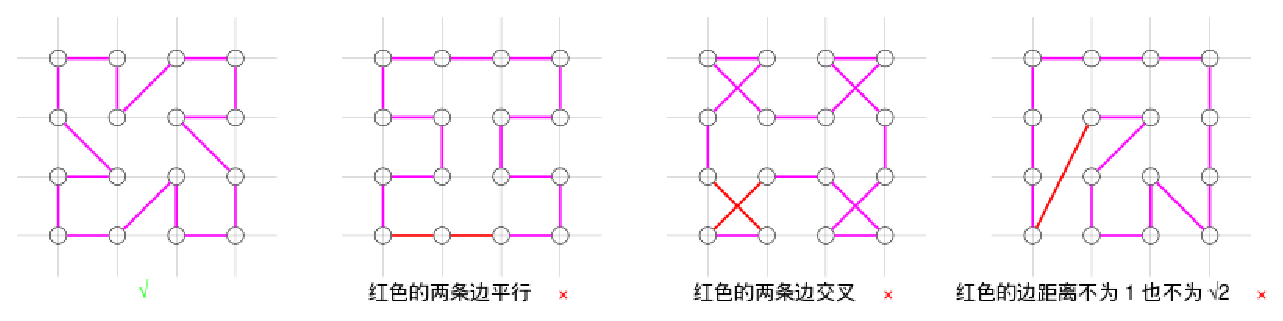
\includegraphics[scale=.4]{assets/hamilton}
		\caption{}
	\end{figure}
}

\sol {\vspace{20pt}
	不妨设 $R \leq C$。容易证明当 $R \leq 3$ 时除 $(R, C) = (2, 2)$ 有平凡解外其余情况都无解,暴搜知 $(R, C) = (5, 5)$ 时无解。\pause

	其余情况均可构造解。我们增强条件,希望从 $(0, 0)$ 开始的前两步分别是右、上。根据下图可知我们可以从 $(R, C)$ 的答案归纳得到 $(R + 4, C + 4)$ 的答案。\pause

	\begin{figure}
		\centering
		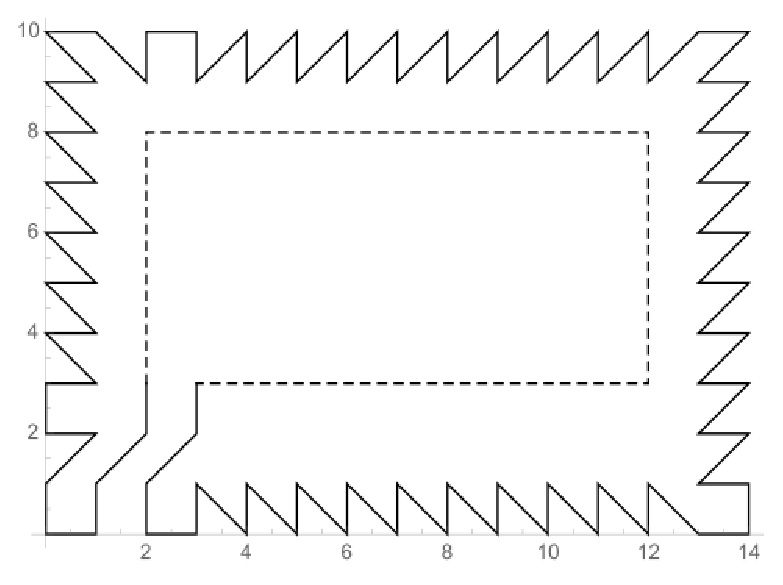
\includegraphics[scale=.35]{assets/enlarge4}
		\caption{}
	\end{figure}
}

\sol {
	于是只需考虑 $4 \leq R \leq 7$ 的情形以及 $(R, C) = (9, 9)$。这些情况可以通过手玩、搜索等方法来完成。
}

% 3
\subsection{Pattern Lock (改编版)}

\subsubsection{JSCPC\,2021\,D (Codeforces\,Gym 103495\,D)}

\frame {\vspace{20pt}
	给定\textsl{完全图} $G = (V, E)$,其中 $V = \bigl\{ (i, j) \bigm| 0 \leq i \leq C - 1, \break \text{$0 \leq j \leq R - 1$ 且 $i, j$ 为整数} \bigr\}$。你需要找到 $G$ 的一个 Hamilton 圈,满足\textsl{视每条边为直线段}后:
	\begin{itemize}
		\item 对任意点 $v \in V$,它关联的两条边构成一个锐角。
		\item 每一条边不能经过除端点外的其它顶点。
	\end{itemize}
	或说明其不存在。{\color{fuchsia}$R \times C \leq 10^6$。}\pausex

	\begin{figure}[htb]
		\centering
		\begin{tikzpicture}
			\fill[nearly opaque, white] (-0.35, -0.35) rectangle (1.35, 1.35);
			\draw[help lines, step=1] (-0.35, -0.35) grid (1.35, 1.35);
			\begin{scope}[circle, minimum size=6pt, every node/.style=draw]
				\node (A) at (0, 0) {};
				\node (B) at (1, 0) {};
				\node (C) at (0, 1) {};
				\node (D) at (1, 1) {};
			\end{scope}
			\draw[semithick, fuchsia] (A) -- (B) -- (C) -- (D) -- (A);
		\end{tikzpicture}
		\caption{}
	\end{figure}
}

\sol {\vspace{12pt}
	\compress{-4pt}{故技重施。\!仍然考虑通过 $(R, C)$ 的解得到 $(R + 4, C + 4)$ 的解。}\pause

	\begin{figure}[htb]
		\centering
		\begin{tikzpicture}[x=.6cm, y=.6cm]
			\fill[nearly opaque, white] (-0.5, -0.5) rectangle (12.5, 8.5);
			\draw[help lines, step=1] (-0.5, -0.5) grid (12.5, 8.5);
			\begin{scope}[circle, minimum size=3pt]
				\node foreach \x in {0,...,12} foreach \y in {0,...,8} [draw] (\x v\y) at (\x, \y) {};
			\end{scope}
			\draw[fuchsia]
					(4v8) -- (4v7) -- (5v8) -- (5v7) -- (6v8) -- (6v7) -- (7v8) -- (7v7)
				 -- (8v8) -- (8v7) -- (9v8) -- (9v7) -- (10v8) -- (10v7) -- (12v8) -- (11v8)
				 -- (12v7) -- (11v7) -- (12v6) -- (11v6) -- (12v5) -- (11v5) -- (12v4) -- (11v4)
				 -- (12v3) -- (11v3) -- (12v2) -- (11v2) -- (12v0) -- (12v1) -- (11v0) -- (11v1)
				 -- (10v0) -- (10v1) -- (9v0) -- (9v1) -- (8v0) -- (8v1) -- (7v0) -- (7v1)
				 -- (6v0) -- (6v1) -- (5v0) -- (5v1) -- (4v0) -- (4v1) -- (3v0) -- (3v1)
				 -- (2v0) -- (2v1) -- (0v0) -- (1v0) -- (0v1) -- (1v1) -- (0v2) -- (1v2)
				 -- (0v3) -- (1v3) -- (0v4) -- (1v4) -- (0v5) -- (1v5) -- (0v6) -- (1v6)
				 -- (0v8) -- (0v7);
			\only<2-3>{
				\draw[fuchsia] (0v7) -- (1v8) -- (1v7) -- (2v8) -- (2v7) -- (3v8) -- (3v7) -- (4v8);
			}
			\only<3>{
				\draw[red] (2v2) -- (3v2);
			}
			\only<3->{
				\draw[red, dash pattern=on 1.5pt off 1.5pt] (2v2) -- (2.666667, 3.666667) (3v2) -- (2.333333, 3.666667);
			}
			\only<4->{
				\draw[semithick, blue] (2v2) -- (3v8);
				\draw[semithick, blue] (3v2) -- (4v8);
				\draw[fuchsia] (1v8) -- (1v7) -- (2v8) (2v7) -- (3v8);
				\draw[semithick, orange] (0v7) -- (2v8) (1v8) -- (3v7) -- (2v7);
			}
		\end{tikzpicture}
	\end{figure}
}


	\section{序列类} % 4 ~ 7
	% 4
\subsection{Secret of Tianqiu Valley}

\subsubsection{ICPC\,Asia\,Nanjing\,Regional\,2021\,L (Codeforces\,Gym 103470\,L)}

\frame {
	有 $n$ 盏灯排成\emm{\textsl{一圈}},标号为 $0, 1, \ldots, n - 1$。给定每盏灯的初始状态 (开或关),你可以进行若干次如下操作:
	\begin{itemize}
		\item 选择一盏\textsl{关闭}的灯 (设标号为 $i$),\emm\textsl{切换}标号为 $i - 1, i, i + 1$ 的灯的状态 (下标在 $\operatorname{mod} n$ 意义下)。
	\end{itemize}

	你需要在 $2 n$ 次操作以内 (含) 将所有灯点亮或说明无法做到。{\color{fuchsia}$3 \leq n \leq 10^5$。}
}

\sol {
	忽略``只能选择关闭的灯''的限制,容易发现这是一个 $\f F_2$ 下线性方程组问题:

	用 $1$ 表示关闭,$0$ 表示开启。设 $\v s$ 为状态向量,$\v t$ 为操作向量,$\vbox to22pt{}\m A = \left(\begin{smallmatrix}
		1\, & 1 & & & 1 \\
		1\, & 1 & 1 & & \\
		& 1 & 1 & {\tiny\mathstrut\Sddots{-1.5pt}} & \\
		& & {\tiny\mathstrut\Sddots{-1.5pt}} & {\tiny\mathstrut\Sddots{-1.5pt}} & 1 \\
		1\, &  &  & 1 & 1 \\
	\end{smallmatrix}\right)$,则\vspace{-4pt}\begin{equation}\label{eq:light}\v s = \m A \v t.\end{equation}

	\vspace{-8pt}\pause
	解方程 \eqref{eq:light} 后,不妨设 $\v t$ 为一组解,我们说明,只要解存在,我们一定可以在 $2 \abs {\v t}$ 步内操作完成,其中 $\abs {\v t}$ 表示 $\v t$ 中 $1$ 的数量。
}

\sol {
	不妨设{\only<2,4,6>{\color{red}}不存在 $i$ 使得 $\v s_i = \v t_i = 1$},且存在 $j$ 使得 $\v s_j = 1$。

	\begin{figure}[htb]
		\centering
		\begin{tikzpicture}[x=.75cm, y=.75cm]
			\fill[nearly opaque, white] (-4, -1.75) rectangle (3.75, 2.75);
			\draw node at (-3.5, 1.5) {$\v s$:} node at (-3.5, -1) {$\v t$:} node at (-0.5, 2.4) {\small $j$};
			% nodes
			\only<7,9->{
				\fill[nearly transparent, fuchsia] (-1, 1) rectangle (0, 2);
				\node at (-0.5, 1.5) {$0$};
			}
			\only<-6,8>{
				\fill[nearly transparent, orange] (-1, 1) rectangle (0, 2);
				\node at (-0.5, 1.5) {$1$};
			}

			\only<4-6,8->{
				\fill[nearly transparent, fuchsia] (0, 1) rectangle (1, 2);
				\node at (0.5, 1.5) {$0$};
			}
			\only<7>{
				\fill[nearly transparent, orange] (0, 1) rectangle (1, 2);
				\node at (0.5, 1.5) {$1$};
			}

			\only<6-7,9->{
				\fill[nearly transparent, fuchsia] (1, 1) rectangle (2, 2);
				\node at (1.5, 1.5) {$0$};
			}
			\only<8>{
				\fill[nearly transparent, orange] (1, 1) rectangle (2, 2);
				\node at (1.5, 1.5) {$1$};
			}

			\only<3->{
				\fill[nearly transparent, fuchsia] (-2, -1.5) rectangle (-1, -0.5);
				\node at (-1.5, -1) {$0$};
			}

			\only<2-6,9->{
				\fill[nearly transparent, fuchsia] (-1, -1.5) rectangle (0, -0.5);
				\node at (-0.5, -1) {$0$};
			}
			\only<7-8>{
				\fill[nearly transparent, orange] (-1, -1.5) rectangle (0, -0.5);
				\node at (-0.5, -1) {$1$};
			}

			\only<8->{
				\fill[nearly transparent, fuchsia] (0, -1.5) rectangle (1, -0.5);
				\node at (0.5, -1) {$0$};
			}
			\only<3-7>{
				\fill[nearly transparent, orange] (0, -1.5) rectangle (1, -0.5);
				\node at (0.5, -1) {$1$};
			}

			\only<9->{
				\fill[nearly transparent, fuchsia] (1, -1.5) rectangle (2, -0.5);
				\node at (1.5, -1) {$0$};
			}
			\only<5-8>{
				\fill[nearly transparent, orange] (1, -1.5) rectangle (2, -0.5);
				\node at (1.5, -1) {$1$};
			}
			% trans
			\only<2>{
				\draw[->] (-0.5, 0.8) -- (-0.5, -0.3);
			}
			\only<3>{
				\draw (-0.5, 0.8) -- (-0.5, -0.3) (-0.6, 0.8) -- (-1.4, -0.3) (-0.4, 0.8) -- (0.4, -0.3);
				\node at (-0.3, 0.1) {\footnotesize $\m A$};
			}
			\only<4>{
				\draw[->] (0.5, -0.3) -- (0.5, 0.8);
			}
			\only<5>{
				\draw (0.5, 0.8) -- (0.5, -0.3) (0.4, 0.8) -- (-0.4, -0.3) (0.6, 0.8) -- (1.4, -0.3);
				\node at (0.7, 0.1) {\footnotesize $\m A$};
			}
			\only<6>{
				\draw[->] (1.5, -0.3) -- (1.5, 0.8);
			}
			\only<7>{
				\draw[radius=0.333333] (-0.5, 1.5) circle {} (-0.5, -1) circle;
				\draw[->] (-0.5, -0.3) -- (-0.5, 0.8);
				\draw[->] (-0.6, -0.3) -- (-1.4, 0.8);
				\draw[->] (-0.4, -0.3) -- (0.4, 0.8);
			}
			\only<8>{
				\draw[radius=0.333333] (0.5, 1.5) circle {} (0.5, -1) circle;
				\draw[->] (0.5, -0.3) -- (0.5, 0.8);
				\draw[->] (0.4, -0.3) -- (-0.4, 0.8);
				\draw[->] (0.6, -0.3) -- (1.4, 0.8);
			}
			\only<9>{
				\draw[radius=0.333333] (-0.5, 1.5) circle {} (-0.5, -1) circle {} (1.5, 1.5) circle {} (1.5, -1) circle;
				\draw[->] (-0.5, -0.3) -- (-0.5, 0.8);
				\draw[->] (-0.6, -0.3) -- (-1.4, 0.8);
				\draw[->] (-0.4, -0.3) -- (0.4, 0.8);
				\draw[->] (1.5, -0.3) -- (1.5, 0.8);
				\draw[->] (1.4, -0.3) -- (0.6, 0.8);
				\draw[->] (1.6, -0.3) -- (2.4, 0.8);
			}
			% borders
			\draw (-2.5, 2) -- (3.5, 2) (-2.5, 1) -- (3.5, 1) (-2.5, -0.5) -- (3.5, -0.5) (-2.5, -1.5) -- (3.5, -1.5);
			\draw foreach \x in {-2,...,3} {(\x, 1) -- +(0, 1) (\x, -1.5) -- +(0, 1)};
		\end{tikzpicture}
	\end{figure}
}

% 5
\subsection{开关}

\subsubsection{原创题}

\frame {
	有 $n$ 盏灯排成一列,标号为 $1, 2, \ldots, n$,给定初始状态 $\v s$ 和目标状态 $\v t$,你可以进行若干次如下操作:
	\begin{itemize}
		\item 选择一段区间 $l, r$ ($1 \leq l \leq r \leq n$),\emm{\textsl{你需要满足区间内点亮的灯数等于关闭的灯数}},然后切换该区间内\textsl{所有}灯的状态。
	\end{itemize}

	你需要在满足 $\sum (r - l + 1) \leq 6\,666\,666$ 的条件下将 $\v s$ 变成	$\v t$ 或说明无法做到。{\color{fuchsia}$1 \leq n \leq 10^5$。}
}

\sol {
	\compress{-4pt}{不难发现操作不改变亮着的灯的总数,\!所以当 $\abs {\v s} \neq \abs {\v t}$ 时无解。}\pause

	用 $0, 1$ 表示两种状态,注意到操作可逆,故不妨设 $\v t$ 有序 (所有 $0$ 都在 $1$ 的左边)。\pause

	先考虑如何将 $\underbrace{11\ldots1}_n\underbrace{00\ldots0}_m$ 变成 $\underbrace{00\ldots0}_m\underbrace{11\ldots1}_n$。
}

\sol {\vspace{8pt}
	{\color{gray}先考虑如何将 $\underbrace{11\ldots1}_n\underbrace{00\ldots0}_m$ 变成 $\underbrace{00\ldots0}_m\underbrace{11\ldots1}_n$。}

	将 $0$ 视作 $\to$,$1$ 视作 $\downarrow$,则一个序列可以看成一个 $n$ 行 $m$ 列的 (从左上角到右下角的) 格路:

	\begin{figure}[htb]
		\centering
		\begin{tikzpicture}[x=.6cm, y=.6cm]
			\fill[nearly opaque, white] (-0.25, -0.25) rectangle (13.25, 5.25);
			\draw[help lines, step=1] (0, 0) grid (13, 5);
			\draw[->, semithick, fuchsia] (0, 5) -| (13, 0);
			\draw[decorate, decoration=brace] (-3pt, 0) -- +(0, 5) node[midway, left, inner sep=5pt] {\small $n$};
			\draw[decorate, decoration={brace,mirror}] (0, -3pt) -- +(13, 0) node[midway, below, inner sep=5pt] {\small $m$};
			\only<1>{
				\draw[->, semithick, blue] (0, 5) |- (13, 0);
			}
			\only<2->{
				\fill[nearly transparent, orange] (0, 0) rectangle (5, 5);
			}
			\only<2>{
				\draw[->, semithick, blue] (0, 5) -| (5, 0) -- (13, 0);
			}
			\only<3->{
				\fill[nearly transparent, aqua] (5, 0) rectangle (10, 5);
			}
			\only<3>{
				\draw[->, semithick, blue] (0, 5) -| (10, 0) -- (13, 0);
			}
			\only<4->{
				\fill[nearly transparent, properpink] (10, 0) rectangle (13, 3);
			}
			\only<4>{
				\draw[->, semithick, blue] (0, 5) -| (10, 3) -| (13, 0);
			}
			\only<5->{
				\fill[nearly transparent, yellow] (10, 3) rectangle (12, 5);
			}
			\only<5>{
				\draw[->, semithick, blue] (0, 5) -| (12, 3) -| (13, 0);
			}
			\only<6->{
				\fill[nearly transparent, properpurple] (12, 3) rectangle (13, 4);
			}
			\only<6>{
				\draw[->, semithick, blue] (0, 5) -| (12, 4) -| (13, 0);
			}
			\only<7->{
				\fill[nearly transparent, red] (12, 4) rectangle (13, 5);
			}
			\only<7>{
				\draw[->, semithick, blue] (0, 5) -| (13, 0);
			}
		\end{tikzpicture}
	\end{figure}
}

\sol {
	\begin{figure}[htb]
		\centering
		\begin{tikzpicture}[x=.6cm, y=.6cm]
			\fill[nearly opaque, white] (-0.25, -1) rectangle (13.25, 5.25);
			\draw[help lines, step=1] (0, 0) grid (13, 5);
			\draw[decorate, decoration=brace] (-3pt, 0) -- +(0, 5) node[midway, left, inner sep=5pt] {\small $n$};
			\draw[decorate, decoration={brace,mirror}] (0, -3pt) -- +(13, 0) node[midway, below, inner sep=5pt] {\small $m$};
			\fill[nearly transparent, orange] (0, 0) rectangle (5, 5);
			\draw[very thick, orange] (0, 5) -- (5, 5);
			\fill[nearly transparent, aqua] (5, 0) rectangle (10, 5);
			\draw[very thick, aqua] (5, 5) -- (10, 5);
			\fill[nearly transparent, properpink] (10, 0) rectangle (13, 3);
			\draw[very thick, properpink] (13, 0) -- (13, 3);
			\fill[nearly transparent, yellow] (10, 3) rectangle (12, 5);
			\draw[very thick, yellow] (10, 5) -- (12, 5);
			\fill[nearly transparent, properpurple] (12, 3) rectangle (13, 4);
			\draw[very thick, properpurple] (13, 3) -- (13, 4);
			\fill[nearly transparent, red] (12, 4) rectangle (13, 5);
			\draw[very thick, red] (12, 5) -- (13, 5);
		\end{tikzpicture}
		\caption{}
	\end{figure}

	\vspace{-8pt}
	这样操作的费用为图中所有正方形的边长之和的 $2$ 倍,这个值不超过 $2 (n + m - 1)$。
}

\sol {\vspace{12pt}
	对于一般的情形,找到类似的 1/0 连续段,然后分治处理。

	\begin{figure}[htb]
		\centering
		\begin{tikzpicture}[x=.6cm, y=.6cm]
			\useasboundingbox (-0.5, -0.5) rectangle (12, 7.75);
			\fill[nearly opaque, white] (-0.5, -0.5) rectangle (12, 8);
			\draw[->] (-0.5, 0) -- (11.5, 0) node[right, inner sep=3pt] {\small $x$};
			\draw[->] (0, -0.5) -- (0, 7.5) node[above, inner sep=3pt] {\small $y$};
			\draw[->, semithick, fuchsia] (0, 7) -- (11, 7) -- (11, 0);
			\only<1>{
				\draw[->, semithick, blue]
					(0, 7) -| (0.88, 6.69) -| (2.34, 5.81) -| (4.14, 4.76)
				 -| (4.84, 3.83) -| (6.1, 2.07) -| (8, 1.75) -| (9.12, 0.29) -| (11, 0);
			}
			\only<2->{
				\fill[nearly transparent, orange] (0.88, 6.69) rectangle (2.34, 7);
			}
			\only<2>{
				\draw[->, semithick, blue]
					(0, 7) -| (2.34, 5.81) -| (4.14, 4.76) -| (4.84, 3.83)
				 -| (6.1, 2.07) -| (8, 1.75) -| (9.12, 0.29) -| (11, 0);
			}
			\only<3->{
				\fill[nearly transparent, aqua] (4.14, 4.76) rectangle (4.84, 5.81);
			}
			\only<3>{
				\draw[->, semithick, blue]
					(0, 7) -| (2.34, 5.81) -| (4.84, 3.83) -| (6.1, 2.07)
				 -| (8, 1.75) -| (9.12, 0.29) -| (11, 0);
			}
			\only<4->{
				\fill[nearly transparent, properpink] (2.34, 5.81) rectangle (4.84, 7);
			}
			\only<4>{
				\draw[->, semithick, blue] (0, 7) -| (4.84, 3.83) -| (6.1, 2.07) -| (8, 1.75) -| (9.12, 0.29) -| (11, 0);
			}
			\only<5->{
				\fill[nearly transparent, yellow] (6.1, 2.07) rectangle (8, 3.83);
			}
			\only<5>{
				\draw[->, semithick, blue] (0, 7) -| (4.84, 3.83) -| (8, 1.75) -| (9.12, 0.29) -| (11, 0);
			}
			\only<6->{
				\fill[nearly transparent, properpurple] (9.12, 0.29) rectangle (11, 1.75);
			}
			\only<6>{
				\draw[->, semithick, blue] (0, 7) -| (4.84, 3.83) -| (8, 1.75) -| (11, 0);
			}
			\only<7->{
				\fill[nearly transparent, red] (8, 1.75) rectangle (11, 3.83);
			}
			\only<7>{
				\draw[->, semithick, blue] (0, 7) -| (4.84, 3.83) -| (11, 0);
			}
			\only<8->{
				\fill[nearly transparent, green] (4.84, 3.83) rectangle (11, 7);
			}
			\only<8->{
				\draw[->, semithick, blue] (0, 7) -| (11, 0);
			}
		\end{tikzpicture}
	\end{figure}

	\vspace{-8pt}
	\onslide<9>{不难发现,$\sum (r - l) = O(n \log n)$。}
}

% 6
\subsection{Quick sort}

\subsubsection{ROI\,2018 D2T3 (Codeforces\,Gym 102154\,C)}

\frame {\vspace{24pt}
	给定一个排列 $\v p = \left[ p_1, p_2, \ldots, p_n \right]$。对奇偶性不同的整数 $l, r$ ($1 \leq l < r \leq n$),定义操作 $S(l, r)$ 为:
	\begin{itemize}
		\item \compress{-12pt}{将 $p_l, p_{l+1}, \ldots, p_r$ 重排为 $p_{l+1}, p_{l+3}, \ldots, p_r, p_l, p_{l+2}, \ldots, p_{r-1}$。}
	\end{itemize}

	你需要构造一种操作序列将 $\v p$ 排序。\!{\color{fuchsia}$1 \mathbin\leq n \mathbin\leq 3000$,\!操作次数\break 不超过 $15\,000$。}\pausex

	\begin{figure}[htb]
		\centering
		\begin{tikzpicture}[x=.6cm, y=.6cm]
			\useasboundingbox (-4, -2) rectangle (4, 2);
			\fill[nearly opaque, white] (-4.75, -2.25) rectangle (4.75, 2.25);
			\draw (-4.5, 2) -- (4.5, 2) (-4.5, 1) -- (4.5, 1) (-4.5, -1) -- (4.5, -1) (-4.5, -2) -- (4.5, -2);
			\draw foreach \x in {-4,...,4} {(\x, 1) -- +(0, 1) (\x, -2) -- +(0, 1)};
			\begin{scope}[nearly transparent]
				\fill[red]			(-4, -2) rectangle +(1, 1) (-3, 1) rectangle +(1, 1);
				\fill[orange]		(-3, -2) rectangle +(1, 1) (-1, 1) rectangle +(1, 1);
				\fill[yellow]		(-2, -2) rectangle +(1, 1) ( 1, 1) rectangle +(1, 1);
				\fill[green]		(-1, -2) rectangle +(1, 1) ( 3, 1) rectangle +(1, 1);
				\fill[aqua]			( 0, -2) rectangle +(1, 1) (-4, 1) rectangle +(1, 1);
				\fill[blue]			( 1, -2) rectangle +(1, 1) (-2, 1) rectangle +(1, 1);
				\fill[properpurple]	( 2, -2) rectangle +(1, 1) ( 0, 1) rectangle +(1, 1);
				\fill[fuchsia]		( 3, -2) rectangle +(1, 1) ( 2, 1) rectangle +(1, 1);
			\end{scope}
			\begin{scope}[->]
				\draw (-2.5, 0.8) -- (-3.5, -0.8);
				\draw (-0.5, 0.8) -- (-2.5, -0.8);
				\draw ( 1.5, 0.8) -- (-1.5, -0.8);
				\draw ( 3.5, 0.8) -- (-0.5, -0.8);
				\draw (-3.5, 0.8) -- ( 0.5, -0.8);
				\draw (-1.5, 0.8) -- ( 1.5, -0.8);
				\draw ( 0.5, 0.8) -- ( 2.5, -0.8);
				\draw ( 2.5, 0.8) -- ( 3.5, -0.8);
			\end{scope}
		\end{tikzpicture}
		\caption{}
	\end{figure}
}

\sol {
	考虑按照 $1 \sim n$ 的顺序将对应数复位。设我们需要将 $v$ 从位置 $p$ 移到位置 $1$。\pause

	可以通过一次操作将其从位置移到 $\left\lceil \frac p2 \right\rceil$。\pause

	于是移动第 $i$ 个数的期望步数为 $\displaystyle \frac 1 {n - i + 1} \sum\limits_{k=1}^{n-i+1} \log k =\break O \bigl( \log (n - i + 1) \bigr)$,总步数为 $\displaystyle \frac 1n \sum_{i=1}^n \log i = O(n \log n)$,无法通过。
}

\sol {\vspace{16pt}
	\emm{\textsl{操作为置换,而置换构成群}}。

	\begin{figure}[htb]
		\centering
		\begin{tikzpicture}[x=.6cm, y=.6cm]
			\useasboundingbox (-4, -2) rectangle (4, 2);
			\fill[nearly opaque, white] (-4.75, -2.25) rectangle (4.75, 2.25);
			\draw (-4.5, 2) -- (4.5, 2) (-4.5, 1) -- (4.5, 1) (-4.5, -1) -- (4.5, -1) (-4.5, -2) -- (4.5, -2);
			\draw foreach \x in {-4,...,4} {(\x, 1) -- +(0, 1) (\x, -2) -- +(0, 1)};
			\begin{scope}[nearly transparent]
				\fill[red]			(-4, -2) rectangle +(1, 1) (-3, 1) rectangle +(1, 1);
				\fill[orange]		(-3, -2) rectangle +(1, 1) (-1, 1) rectangle +(1, 1);
				\fill[yellow]		(-2, -2) rectangle +(1, 1) ( 1, 1) rectangle +(1, 1);
				\fill[green]		(-1, -2) rectangle +(1, 1) ( 3, 1) rectangle +(1, 1);
				\fill[aqua]			( 0, -2) rectangle +(1, 1) (-4, 1) rectangle +(1, 1);
				\fill[blue]			( 1, -2) rectangle +(1, 1) (-2, 1) rectangle +(1, 1);
				\fill[properpurple]	( 2, -2) rectangle +(1, 1) ( 0, 1) rectangle +(1, 1);
				\fill[fuchsia]		( 3, -2) rectangle +(1, 1) ( 2, 1) rectangle +(1, 1);
			\end{scope}
			\alt<1>{\begin{scope}[->]}{\begin{scope}[<-, red, semithick]}
				\draw (-2.5, 0.8) -- (-3.5, -0.8);
				\draw (-0.5, 0.8) -- (-2.5, -0.8);
				\draw ( 1.5, 0.8) -- (-1.5, -0.8);
				\draw ( 3.5, 0.8) -- (-0.5, -0.8);
				\draw (-3.5, 0.8) -- ( 0.5, -0.8);
				\draw (-1.5, 0.8) -- ( 1.5, -0.8);
				\draw ( 0.5, 0.8) -- ( 2.5, -0.8);
				\draw ( 2.5, 0.8) -- ( 3.5, -0.8);
			\end{scope}
		\end{tikzpicture}
	\end{figure}

	\onslide<3->{从 $p$ 到 $1$ 的步数:$\log p \longrightarrow \log n - \log (n - p)$}

	\onslide<4->{移动第 $i$ 个数的期望步数:\vspace{-8pt}\[ \frac 1 {n - i + 1} \sum_{k=1}^{n-i+1} \bigl( \log(n-i+1) - \log(n-i+1-k) \bigr) = O(1). \]}

	\vspace{-16pt}
	\onslide<5->{通过随机操作随机化初始排列,总步数期望为 $2 n + O(1)$。}
}

% 7
\subsection{Balance the Cards}

\subsubsection{Codeforces\,Round \texttt\#712\,F (Codeforces 1503\,F)}

\frame {\vspace{8pt}\footnotesize
	称一个由\textsl{非零整数}构成的序列 $\left[ a_1, a_2, \ldots, a_n \right]$ 是``\textsl{平衡的}'',当且仅当其满足如下三者之一:
	\begin{itemize}
		\item $n = 0$;
		\item \compress{-20pt}{存在 $1 \leq k < n$ 使得 $\left[ a_1, a_2, \ldots, a_k \right]$ 和 $\left[ a_{k+1}, a_{k+2}, \ldots, a_n \right]$ 都是``平衡的'';}
		\item $a_1 = - a_n > 0$ 且 $\left[ a_2, a_3, \ldots, a_{n-1} \right]$ 是``平衡的''。
	\end{itemize}

	给定 $2 n$ 个二元组 $\left( u_i, v_i \right)$,保证 $\left\{ u_1, u_2, \ldots, u_{2 n} \right\} = \left\{ v_1, v_2, \ldots, v_{2 n} \right\} =\break \left\{ 1, -1, 2, -2, \ldots, n, -n \right\}$,你需要找到一个大小为 $2 n$ 的排列 $p_1, p_2, \ldots, p_{2 n}$,使得下列两个条件同时成立:
	\begin{itemize}
		\item $\left[ u_{p_1}, u_{p_2}, \ldots, u_{p_{2 n}} \right]$ 是``平衡的'';
		\item $\left[ v_{p_1}, v_{p_2}, \ldots, v_{p_{2 n}} \right]$ 是``平衡的''。
	\end{itemize}

	给出一组构造,或说明无解。{\color{fuchsia}$1 \leq n \leq 2 \times 10^5$。}
}

\newdimen\hzk
\sol {
	\alt<9->{
		\vspace{8pt}
		\begin{figure}[htb]
			\centering
			\begin{tikzpicture}[x=.75cm, y=.75cm]
				\useasboundingbox (-0.5, -2.25) rectangle (11.75, 3.5);
				\fill[nearly opaque, white] (-0.5, -2.5) rectangle (11.75, 3);
				\hzk0.46875cm
				\begin{scope}[semithick, start angle=180, end angle=0]
					\draw[fuchsia]			(0,    0) arc[radius=3\hzk];
					\draw[blue]				(7.5,  0) arc[radius=1\hzk];
					\draw[orange]			(6.25, 0) arc[radius=3\hzk];
					\draw[red]				(1.25, 0) arc[radius=1\hzk];
					\draw[green!80!black]	(5,    0) arc[radius=5\hzk];
				\end{scope}
				\begin{scope}[semithick, start angle=180, end angle=360]
					\draw[fuchsia]			(5,    0) arc[radius=1\hzk];
					\draw[blue]				(7.5,  0) arc[radius=3\hzk];
					\draw[orange]			(0,    0) arc[radius=1\hzk];
					\draw[red]				(2.5,  0) arc[radius=1\hzk];
					\draw[green!80!black]	(8.75, 0) arc[radius=1\hzk];
				\end{scope}
				\coordinate (U0) at ( 3\hzk, 3\hzk);
				\coordinate (U1) at (13\hzk, 1\hzk);
				\coordinate (U2) at (13\hzk, 3\hzk);
				\coordinate (U3) at ( 3\hzk, 1\hzk);
				\coordinate (U4) at (13\hzk, 5\hzk);
				\coordinate (D0) at ( 9\hzk,-1\hzk);
				\coordinate (D1) at (15\hzk,-3\hzk);
				\coordinate (D2) at ( 1\hzk,-1\hzk);
				\coordinate (D3) at ( 5\hzk,-1\hzk);
				\coordinate (D4) at (15\hzk,-1\hzk);
				\begin{scope}[->, tips=proper, semithick]
					\path[fuchsia]			(U0) +(-.06, 0) -- +(+.06, 0);
					\path[blue]				(U1) +(-.06, 0) -- +(+.06, 0);
					\path[orange]			(U2) +(+.06, 0) -- +(-.06, 0);
					\path[red]				(U3) +(+.06, 0) -- +(-.06, 0);
					\path[green!80!black]	(U4) +(-.06, 0) -- +(+.06, 0);
					\path[fuchsia]			(D0) +(+.06, 0) -- +(-.06, 0);
					\path[blue]				(D1) +(+.06, 0) -- +(-.06, 0);
					\path[orange]			(D2) +(+.06, 0) -- +(-.06, 0);
					\path[red]				(D3) +(+.06, 0) -- +(-.06, 0);
					\path[green!80!black]	(D4) +(-.06, 0) -- +(+.06, 0);
				\end{scope}
				\begin{scope}[inner sep=3pt]
					\node[above, fuchsia]			at (U0) {\footnotesize 顺};
					\node[above, blue]				at (U1) {\footnotesize 顺};
					\node[above, orange]			at (U2) {\footnotesize 逆};
					\node[above, red]				at (U3) {\footnotesize 逆};
					\node[above, green!80!black]	at (U4) {\footnotesize 顺};
					\node[below, fuchsia]			at (D0) {\footnotesize 顺};
					\node[below, blue]				at (D1) {\footnotesize 顺};
					\node[below, orange]			at (D2) {\footnotesize 顺};
					\node[below, red]				at (D3) {\footnotesize 顺};
					\node[below, green!80!black]	at (D4) {\footnotesize 逆};
				\end{scope}
			\end{tikzpicture}
			\caption{}
		\end{figure}

		\vspace{-16pt}
		\begin{itemize}
			\item 该图的连通分量由输入唯一确定。
			\item<10-> 在解中,每个连通分量构成简单闭曲线,故每个圈中\textsl{顺时针弧}的数量比\textsl{逆时针弧}的数量\textsl{恰好多 $2$}。
		\end{itemize}
	}{
		\vspace{12pt}
		``平衡''序列的定义非常像括号序列。\pause

		将 $x > 0$ 看作一种颜色的 \texttt(,$-x$ 看成对应颜色的 \texttt)。\pause

		\begin{figure}[htb]
			\centering
			\begin{tikzpicture}[x=.75cm, y=.75cm]
				\useasboundingbox (-0.5, -2) rectangle (11.75, 3.5);
				\fill[nearly opaque, white] (-0.5, -2.5) rectangle (11.75, 3.75);
				\only<-5>{
					\begin{scope}[inner sep=3pt, rectangle split, rectangle split parts=2, every node/.style=draw]
						\node (0) at (0,    0) {\color{fuchsia}\texttt(\nodepart{two}\color{orange}\texttt(};
						\node (1) at (1.25, 0) {\color{red}\texttt(\nodepart{two}\color{orange}\texttt)};
						\node (2) at (2.5,  0) {\color{red}\texttt)\nodepart{two}\color{red}\texttt(};
						\node (3) at (3.75, 0) {\color{fuchsia}\texttt)\nodepart{two}\color{red}\texttt)};
						\node (4) at (5,    0) {\color{green!80!black}\texttt(\nodepart{two}\color{fuchsia}\texttt(};
						\node (5) at (6.25, 0) {\color{orange}\texttt(\nodepart{two}\color{fuchsia}\texttt)};
						\node (6) at (7.5,  0) {\color{blue}\texttt(\nodepart{two}\color{blue}\texttt(};
						\node (7) at (8.75, 0) {\color{blue}\texttt)\nodepart{two}\color{green!80!black}\texttt(};
						\node (8) at (10,   0) {\color{orange}\texttt)\nodepart{two}\color{green!80!black}\texttt)};
						\node (9) at (11.25,0) {\color{green!80!black}\texttt)\nodepart{two}\color{blue}\texttt)};
					\end{scope}
				}
				\hzk0.541265877365cm
				\only<4-5> {
					\begin{scope}[semithick, start angle=150, end angle=30]
						\draw[fuchsia]			(0.north) arc[radius=3\hzk];
						\draw[blue]				(6.north) arc[radius=1\hzk];
						\draw[orange]			(5.north) arc[radius=3\hzk];
						\draw[red]				(1.north) arc[radius=1\hzk];
						\draw[green!80!black]	(4.north) arc[radius=5\hzk];
					\end{scope}
				}
				\only<5> {
					\begin{scope}[semithick, start angle=210, end angle=330]
						\draw[fuchsia]			(4.south) arc[radius=1\hzk];
						\draw[blue]				(6.south) arc[radius=3\hzk];
						\draw[orange]			(0.south) arc[radius=1\hzk];
						\draw[red]				(2.south) arc[radius=1\hzk];
						\draw[green!80!black]	(7.south) arc[radius=1\hzk];
					\end{scope}
				}
				\only<6->{
					\hzk0.46875cm
					\begin{scope}[semithick, start angle=180, end angle=0]
						\draw[fuchsia]			(0,    0) arc[radius=3\hzk];
						\draw[blue]				(7.5,  0) arc[radius=1\hzk];
						\draw[orange]			(6.25, 0) arc[radius=3\hzk];
						\draw[red]				(1.25, 0) arc[radius=1\hzk];
						\draw[green!80!black]	(5,    0) arc[radius=5\hzk];
					\end{scope}
					\begin{scope}[semithick, start angle=180, end angle=360]
						\draw[fuchsia]			(5,    0) arc[radius=1\hzk];
						\draw[blue]				(7.5,  0) arc[radius=3\hzk];
						\draw[orange]			(0,    0) arc[radius=1\hzk];
						\draw[red]				(2.5,  0) arc[radius=1\hzk];
						\draw[green!80!black]	(8.75, 0) arc[radius=1\hzk];
					\end{scope}
					\coordinate (U0) at ( 3\hzk, 3\hzk);
					\coordinate (U1) at (13\hzk, 1\hzk);
					\coordinate (U2) at (13\hzk, 3\hzk);
					\coordinate (U3) at ( 3\hzk, 1\hzk);
					\coordinate (U4) at (13\hzk, 5\hzk);
					\coordinate (D0) at ( 9\hzk,-1\hzk);
					\coordinate (D1) at (15\hzk,-3\hzk);
					\coordinate (D2) at ( 1\hzk,-1\hzk);
					\coordinate (D3) at ( 5\hzk,-1\hzk);
					\coordinate (D4) at (15\hzk,-1\hzk);
					\only<7->{
						\begin{scope}[->, tips=proper, semithick]
							\path[fuchsia]			(U0) +(-.06, 0) -- +(+.06, 0);
							\path[blue]				(U1) +(-.06, 0) -- +(+.06, 0);
							\path[orange]			(U2) +(+.06, 0) -- +(-.06, 0);
							\path[red]				(U3) +(+.06, 0) -- +(-.06, 0);
							\path[green!80!black]	(U4) +(-.06, 0) -- +(+.06, 0);
							\path[fuchsia]			(D0) +(+.06, 0) -- +(-.06, 0);
							\path[blue]				(D1) +(+.06, 0) -- +(-.06, 0);
							\path[orange]			(D2) +(+.06, 0) -- +(-.06, 0);
							\path[red]				(D3) +(+.06, 0) -- +(-.06, 0);
							\path[green!80!black]	(D4) +(-.06, 0) -- +(+.06, 0);
						\end{scope}
					}
					\only<8->{
						\begin{scope}[inner sep=3pt]
							\node[above, fuchsia]			at (U0) {\footnotesize 顺};
							\node[above, blue]				at (U1) {\footnotesize 顺};
							\node[above, orange]			at (U2) {\footnotesize 逆};
							\node[above, red]				at (U3) {\footnotesize 逆};
							\node[above, green!80!black]	at (U4) {\footnotesize 顺};
							\node[below, fuchsia]			at (D0) {\footnotesize 顺};
							\node[below, blue]				at (D1) {\footnotesize 顺};
							\node[below, orange]			at (D2) {\footnotesize 顺};
							\node[below, red]				at (D3) {\footnotesize 顺};
							\node[below, green!80!black]	at (D4) {\footnotesize 逆};
						\end{scope}
					}
				}
			\end{tikzpicture}
		\end{figure}
	}
}

\sol {
	\alt<5->{
		\begin{figure}[htb]
			\centering
			\begin{tikzpicture}[x=.75cm, y=.75cm]
				\useasboundingbox (-0.5, -1.65) rectangle (7.9, 3.75);
				\fill[nearly opaque, white] (-0.5, -1.9) rectangle (7.9, 3.75);
				\draw[densely dotted] (-0.5, 0) -- (7.9, 0);
				\draw[start angle=180, end angle=0, fuchsia] (0, 0) arc[radius=3.5];
				\draw[start angle=180, end angle=360, blue] (0, 0) arc[radius=1];
				\path[->, tips=proper, fuchsia] (3.44, 3.5) -- (3.56, 3.5);
				\path[->, tips=proper, blue] (1.06, -1) -- (0.94, -1);
				\begin{scope}[minimum size=2.5pt, circle, every node/.style=fill]
					\node[red] at (0, 0) {};
					\node[orange] (A) at (7, 0) {};
					\node[orange] (B) at (2, 0) {};
				\end{scope}
				\begin{scope}[semithick]
					\draw[->, orange] (A) -- +(0, -1);
					\draw[<-, orange] (B) -- +(0, 1);
				\end{scope}
				\node at (2.04, 1.15) {\footnotesize\color{orange}$\cdots$};
				\node at (7.04, -1.15) {\footnotesize\color{orange}$\cdots$};
				\only<6->{
					\draw[dashed] (1.6, -0.25) rectangle (2.4, 1.4) node[right] at (2.5, 0.575) {\footnotesize 终点};
					\draw[dashed] (6.6, -1.4) rectangle (7.4, 0.25) node[left] at (6.5, -0.575) {\footnotesize 起点};
					\draw (1.35, -1.65) rectangle (7.65, 1.65);
				}
			\end{tikzpicture}
		\end{figure}

		\onslide<6->{对于一个``顺''``逆''数量相同的序列,可以看成上图中从\textsl{起点}出发向下最后向下回到\textsl{终点}的曲线 ({\color{orange}橙色}部分),\textsl{且起点正上方,终点正下方不能有弧经过}。}
	}{
		\vspace{8pt}
		对于一个给定的``顺''``逆''环状序列,其中``顺''的数量比``逆''多 $2$,能否一定完成构造呢?\pause

		\begin{itemize}
			\item 必然存在两个相邻的``顺'',令其经过最左侧的点。
		\end{itemize}

		\begin{figure}[htb]
			\centering
			\begin{tikzpicture}[x=.75cm, y=.75cm]
				\useasboundingbox (-0.5, -2.15) rectangle (5, 2.5);
				\fill[nearly opaque, white] (-0.5, -2.15) rectangle (5, 2.85);
				\begin{scope}[semithick]
					\draw[fuchsia] (0, 0) arc[start angle=180, end angle=0, radius=2.25];
					\draw[blue] (0, 0) arc[start angle=180, end angle=360, radius=1.4];
					\path[->, tips=proper, fuchsia] (2.19, 2.25) -- (2.31, 2.25);
					\path[->, tips=proper, blue] (1.46, -1.4) -- (1.34, -1.4);
				\end{scope}
				\begin{scope}[inner sep=3pt]
					\node[above, fuchsia] at (2.25, 2.25) {\footnotesize 顺};
					\node[below, blue] at (1.4, -1.4) {\footnotesize 顺};
					\alt<4->{
						\node at (2.84, 0.65) {\footnotesize\color{orange}$\cdots$};
						\node at (4.54, -0.65) {\footnotesize\color{orange}$\cdots$};
					}{
						\node at (2.84, 0.15) {\footnotesize $\cdots$};
						\node at (4.54, -0.15) {\footnotesize $\cdots$};
					}
				\end{scope}
				\begin{scope}[minimum size=2.5pt, circle, every node/.style=fill]
					\node[red] at (0, 0) {};
					\only<4->{
						\node[orange] (A) at (4.5, 0) {};
						\node[orange] (B) at (2.8, 0) {};
					}
				\end{scope}
				\only<4->{
					\draw[->, semithick, orange] (A) -- +(0, -0.5);
					\draw[<-, semithick, orange] (B) -- +(0, 0.5);
				}
			\end{tikzpicture}
		\end{figure}\pause

		\vspace{-12pt}
		\begin{itemize}
			\item 剩下的部分中,``顺''的数量与``逆''的数量恰好相同。
		\end{itemize}
	}
}

\ifpreview\else
\begin{frame}[fragile]
	\vspace{16pt}
	记``顺''为 $+$,``逆''为 $-$。令 $S$ 为所有可构造的 $+/-$ 序列的集合。显然 $[\mskip1mu] \in S$。\pause

	\begin{enumerate}
		\item 若 $s \in S$,则 ${+ s -} \in S$。
	\end{enumerate}

	\begin{figure}[htb]
		\centering
		\begin{tikzpicture}[x=.75cm, y=.75cm]
			\useasboundingbox (-4.75, -3) rectangle (4.75, 3);
			\fill[nearly opaque, white] (-4.75, -3.5) rectangle (4.75, 3.55);
			\draw[densely dotted] (-4.75, 0) -- (4.75, 0);
			\draw (-3.25, -2) rectangle (3.25, 2);
			\alt<3->{
				\begin{scope}[semithick]
					\draw[<-, orange] (A) -- +(0, -1);
					\draw[->, orange] (B) -- +(0, 1);
					\begin{scope}[hzk/.style 2 args={decoration={
						markings, mark=between positions .166667 and .84 step .166667 with {
							##1[semithick, ##2]{>}
						}
					}}]
						\draw[postaction=decorate, hzk={\arrow}{blue}, blue] (A) arc[start angle=0, end angle=180, radius=3.375];
						\draw[postaction=decorate, hzk={\arrowreversed}{fuchsia}, fuchsia] (B) arc[start angle=180, end angle=360, radius=3.375];
					\end{scope}
				\end{scope}
				\begin{scope}[minimum size=2.5pt, circle, every node/.style=fill]
					\node[orange] (A) at (2.5, 0) {};
					\node[orange] (B) at (-2.5, 0) {};
					\node[fuchsia] (C) at (4.25, 0) {};
					\node[blue] (D) at (-4.25, 0) {};
				\end{scope}
				\draw[semithick, densely dashed, orange, postaction=decorate, decoration={
					markings, mark=between positions .254 and .8 step .1618 with {
						\arrowreversed[semithick, orange]{>}
					}
				}] (2.5, -1) .. controls (2.5, -4) and (-2.5, 4) .. (-2.5, 1);
			}{
				\begin{scope}[minimum size=2.5pt, circle, every node/.style=fill]
					\node[fuchsia] (A) at (2.5, 0) {};
					\node[blue] (B) at (-2.5, 0) {};
				\end{scope}
				\begin{scope}[semithick]
					\draw[->, fuchsia] (A) -- +(0, -1);
					\draw[<-, blue] (B) -- +(0, 1);
				\end{scope}
				\draw[semithick, densely dashed, orange, postaction=decorate, decoration={
					markings, mark=between positions .247 and .8 step .1618 with {
						\arrow[semithick, orange]{>}
					}
				}] (2.5, -1) .. controls (2.5, -4) and (-2.5, 4) .. (-2.5, 1);
				\node at (-2.46, 1.15) {\footnotesize\color{blue}$\cdots$};
				\node at (2.54, -1.15) {\footnotesize\color{fuchsia}$\cdots$};
			}
		\end{tikzpicture}
	\end{figure}
\end{frame}

\begin{frame}[fragile]
	\begin{enumerate}
		\setcounter{enumi}{1}
		\item 若 $s \in S$,则 ${- s +} \in S$。
	\end{enumerate}

	\begin{figure}[htb]
		\centering
		\begin{tikzpicture}[x=.75cm, y=.75cm]
			\useasboundingbox (-4.75, -3) rectangle (4.75, 3);
			\fill[nearly opaque, white] (-4.75, -3) rectangle (4.75, 3);
			\draw[densely dotted] (-4.75, 0) -- (4.75, 0);
			\draw (-3.25, -2) rectangle (3.25, 2); % (5 + 1.5) * 4
			\alt<2->{
				\begin{scope}[semithick]
					\draw[<-, orange] (A) -- +(0, -1);
					\draw[->, orange] (B) -- +(0, 1);
					\begin{scope}[hzk/.style 2 args={decoration={
						markings, mark=between positions .166667 and .84 step .166667 with {
							##1[semithick, ##2]{>}
						}
					}}]
						\draw[postaction=decorate, hzk={\arrow}{blue}, blue] (A) -- +(0, 2) arc[start angle=180, end angle=0, radius=.75] -- +(0, -2);
						\draw[postaction=decorate, hzk={\arrowreversed}{fuchsia}, fuchsia] (B) -- +(0, -2) arc[start angle=360, end angle=180, radius=.75] -- +(0, 2);
					\end{scope}
				\end{scope}
				\begin{scope}[minimum size=2.5pt, circle, every node/.style=fill]
					\node[orange] (A) at (2.5, 0) {};
					\node[orange] (B) at (-2.5, 0) {};
					\node[blue] (C) at (4, 0) {};
					\node[fuchsia] (D) at (-4, 0) {};
				\end{scope}
				\draw[semithick, densely dashed, orange, postaction=decorate, decoration={
					markings, mark=between positions .254 and .8 step .1618 with {
						\arrowreversed[semithick, orange]{>}
					}
				}] (2.5, -1) .. controls (2.5, -4) and (-2.5, 4) .. (-2.5, 1);
			}{
				\begin{scope}[minimum size=2.5pt, circle, every node/.style=fill]
					\node[fuchsia] (A) at (2.5, 0) {};
					\node[blue] (B) at (-2.5, 0) {};
				\end{scope}
				\begin{scope}[semithick]
					\draw[->, fuchsia] (A) -- +(0, -1);
					\draw[<-, blue] (B) -- +(0, 1);
				\end{scope}
				\draw[semithick, densely dashed, orange, postaction=decorate, decoration={
					markings, mark=between positions .247 and .8 step .1618 with {
						\arrow[semithick, orange]{>}
					}
				}] (2.5, -1) .. controls (2.5, -4) and (-2.5, 4) .. (-2.5, 1);
				\node at (-2.46, 1.15) {\footnotesize\color{blue}$\cdots$};
				\node at (2.54, -1.15) {\footnotesize\color{fuchsia}$\cdots$};
			}
		\end{tikzpicture}
	\end{figure}
\end{frame}
\fi

\sol {
	\begin{enumerate}
		\setcounter{enumi}{2}
		\item 若 $s, t \in S$,则 $s t \in S$。
	\end{enumerate}

	\begin{figure}[htb]
		\centering
		\begin{tikzpicture}[x=.75cm, y=.75cm]
			\useasboundingbox (-5, -2.5) rectangle (5, 2.5);
			\fill[nearly opaque, white] (-5, -2.5) rectangle (5, 2.5);
			\draw[densely dotted] (-5, 0) -- (5, 0);
			\alt<3->{
				\begin{scope}[shift={(1.25, 0)}]
					\draw (-5.75, -2) rectangle (3.25, 2) (-4.916667, -1) rectangle (-2.083333, 1);
					\begin{scope}[minimum size=2.5pt, circle, every node/.style=fill]
						\node[fuchsia] (A) at (2.5, 0) {};
						\node[orange] (B) at (-2.5, 0) {};
						\node[blue] (C) at (-4.5, 0) {};
						\node[green!80!black] at (-5.333333, 0) {};
					\end{scope}
					\begin{scope}[semithick]
						\draw[->, fuchsia] (A) -- +(0, -1);
						\draw[<-, orange] (B) -- +(0, 0.6);
						\draw[->, orange] (B) -- +(0, -0.6);
						\draw[<-, blue] (C) -- +(0, 0.6);
					\end{scope}
					\begin{scope}[semithick, densely dashed, orange]
						\draw[postaction=decorate, decoration={
							markings, mark=between positions .247 and .8 step .1618 with {
								\arrow[semithick, orange]{>}
							}
						}] (2.5, -1) .. controls (2.5, -4) and (-2.5, 4) .. (-2.5, 1);
						\draw[postaction=decorate, decoration={
							markings, mark=between positions .35 and .8 step .31 with {
								\arrow[semithick, orange]{>}
							}
						}] (-2.5, -0.6) .. controls (-2.5, -1.8) and (-4.5, 1.8) .. (-4.5, 0.6);
						\draw (-2.5, 1) -- (-2.5, 0.6);
					\end{scope}
				\end{scope}
			}{
				\draw (-4.5, -1.5) rectangle (-0.5, 1.5) (0, -1.5) rectangle (4.5, 1.5); % (3 + 1) * 3
				\begin{scope}[minimum size=2.5pt, circle, every node/.style=fill]
					\node[fuchsia] (A) at (-1, 0) {};
					\node[blue] (B) at (-4, 0) {};
					\node[fuchsia] (C) at (4, 0) {};
					\node[blue] (D) at (1, 0) {};
					\only<2->{\node[green!80!black] at (0.25, 0) {};}
				\end{scope}
				\begin{scope}[semithick]
					\draw[->, fuchsia] (A) -- +(0, -1);
					\draw[<-, blue] (B) -- +(0, 1);
					\draw[->, fuchsia] (C) -- +(0, -1);
					\draw[<-, blue] (D) -- +(0, 1);
				\end{scope}
				\begin{scope}[semithick, densely dashed, orange, decoration={
					markings, mark=between positions .247 and .8 step .261 with {
						\arrow[semithick, orange]{>}
					}
				}]
					\draw[postaction=decorate] (4, -1) .. controls (4, -2.5) and (1, 2.5) .. (1, 1);
					\draw[postaction=decorate] (-1, -1) .. controls (-1, -2.5) and (-4, 2.5) .. (-4, 1);
				\end{scope}
				\node at (-3.96, 1.15) {\footnotesize\color{blue}$\cdots$};
				\node at (-0.96, -1.15) {\footnotesize\color{fuchsia}$\cdots$};
				\node at (1.04, 1.15) {\footnotesize\color{blue}$\cdots$};
				\node at (4.04, -1.15) {\footnotesize\color{fuchsia}$\cdots$};
				\only<2->{
					\draw (0.5, -0.1875) rectangle (1, 0.1875);
					\draw[densely dotted]
						(-4.5, -1.5) -- (0.5, -0.1875) (-0.5, -1.5) -- (1, -0.1875)
						(-4.5,  1.5) -- (0.5,  0.1875) (-0.5,  1.5) -- (1,  0.1875);
				}
			}
		\end{tikzpicture}
	\end{figure}
}

\sol {\vspace{12pt}
	因此 $S$ 为所有 $+$ 和 $-$ 数量相同的序列集合。事实上,我们可以通过栈和链表来辅助完成这个构造\only<24->{,时间复杂度 \smash{$O(n)$}}。\pause

	\begin{figure}[htb]
		\centering
		\begin{tikzpicture}[x=.5cm, y=.5cm]
			\useasboundingbox (-0.5, -5) rectangle (16.5, 4.75);
			\fill[nearly opaque, white] (-0.5, -5) rectangle (16.5, 5.25);
			\draw[help lines, step=1] (0, -4) grid (16, 4);
			\draw[->] (-0.5, 0) -- (16.5, 0) node[right, inner sep=3pt] {\small $x$};
			\draw[->] (0, -5) -- (0, 4.5) node[above, inner sep=3pt] {\small $y$};
			\draw[semithick, fuchsia] (0, 0)
				-- ++(1, -1) -- ++(1, 1) -- ++(1, 1) -- ++(1, -1) -- ++(1, 1) -- ++(1, 1) -- ++(1, 1) -- ++(1, -1)
				-- ++(1, -1) -- ++(1, 1) -- ++(1, -1) -- ++(1, 1) -- ++(1, -1) -- ++(1, -1) -- ++(1, 1) -- ++(1, -1);
			\begin{scope}[->, semithick, minimum size=2.5pt, circle, green!80!black, every node/.style=fill]
				\only<3>{\draw (1, 0) -- +(0, -1) node {};}
				\only<4>{\node at (2, 0) {};}
				\only<5>{\draw (3, 0) -- +(0, 1) node {};}
				\only<6-7>{\node at (4, 0) {};}
				\only<8>{\draw (5, 0) -- +(0, 1) node {};}
				\only<9>{\draw (6, 0) -- +(0, 2) node {};}
				\only<10>{\draw (7, 0) -- +(0, 3) node {};}
				\only<11>{\draw (8, 0) -- +(0, 2) node {};}
				\only<12>{\draw (9, 0) -- +(0, 1) node {};}
				\only<13>{\draw (10, 0) -- +(0, 2) node {};}
				\only<14-15>{\draw (11, 0) -- +(0, 1) node {};}
				\only<16>{\draw (12, 0) -- +(0, 2) node {};}
				\only<17-18>{\draw (13, 0) -- +(0, 1) node {};}
				\only<19-20>{\node at (14, 0) {};}
				\only<21>{\draw (15, 0) -- +(0, 1) node {};}
				\only<22->{\node at (16, 0) {};}
			\end{scope}
			\begin{scope}[nearly transparent]
				\only<4-6>{\fill[blue] (0, 0) -- ++(1, -1) -- ++(1, 1) -- cycle;}
				\only<6>{\fill[orange] (2, 0) -- ++(1, 1) -- ++(1, -1) -- cycle;}
				\only<7-19>{\fill[aqua] (0, 0) -- ++(1, -1) -- ++(1, 1) -- ++(1, 1) -- ++(1, -1) -- cycle;}
				\only<11>{\fill[properpink] (6, 2) -- ++(1, 1) -- ++(1, -1) -- cycle;}
				\only<12-14>{\fill[yellow] (5, 1) -- ++(2, 2) -- ++(2, -2) -- cycle;}
				\only<14>{\fill[properpurple] (9, 1) -- ++(1, 1) -- ++(1, -1) -- cycle;}
				\only<15-17>{\fill[red] (5, 1) -- ++(2, 2) -- ++(2, -2) -- ++(1, 1) -- ++(1, -1) -- cycle;}
				\only<17>{\fill[blue] (11, 1) -- ++(1, 1) -- ++(1, -1) -- cycle;}
				\only<18>{\fill[orange] (5, 1) -- ++(2, 2) -- ++(2, -2) -- ++(1, 1) -- ++(1, -1) -- ++(1, 1) -- ++(1, -1) -- cycle;}
				\only<19>{\fill[properpink] (4, 0) -- ++(1, 1) -- ++(2, 2) -- ++(2, -2) -- ++(1, 1) -- ++(1, -1) -- ++(1, 1) -- ++(1, -1) -- ++(1, -1) -- cycle;}
				\only<20-22>{\fill[yellow] (0, 0) -- ++(1, -1) -- ++(1, 1) -- ++(1, 1) -- ++(1, -1) -- ++(1, 1) -- ++(2, 2) -- ++(2, -2) -- ++(1, 1) -- ++(1, -1) -- ++(1, 1) -- ++(1, -1) -- ++(1, -1) -- cycle;}
				\only<22>{\fill[properpurple] (14, 0) -- ++(1, 1) -- ++(1, -1) -- cycle;}
				\only<23->{\fill[red] (0, 0) -- ++(1, -1) -- ++(1, 1) -- ++(1, 1) -- ++(1, -1) -- ++(1, 1) -- ++(2, 2) -- ++(2, -2) -- ++(1, 1) -- ++(1, -1) -- ++(1, 1) -- ++(1, -1) -- ++(1, -1) -- ++(1, 1) -- ++(1, -1) -- cycle;}
			\end{scope}
			\node at (8, -4.75) {\small
				\only<4>{($\color{green!80!black} - +$)}%
				\only<6>{($\color{green!80!black} + -$)}%
				\only<7>{($\color{blue} {-} {+} \color{orange} {+} {-}$)}%
				\only<11>{($\color{green!80!black} + -$)}%
				\only<12>{(${\color{green!80!black} +} {+} {-} {\color{green!80!black} -}$)}%
				\only<14>{($\color{green!80!black} + -$)}%
				\only<15>{($\color{yellow!90!black} {+} {+} {-} {-} \color{properpurple} {+} {-}$)}%
				\only<17>{($\color{green!80!black} + -$)}%
				\only<18>{($\color{red} {+} {+} {-} {-} {+} {-} \color{blue} {+} {-}$)}%
				\only<19>{(${\color{green!80!black} +} {+} {+} {-} {-} {+} {-} {+} {-} {\color{green!80!black} -}$)}%
				\only<20>{($\color{aqua} {-} {+} {+} {-} \color{properpink} {+} {+} {+} {-} {-} {+} {-} {+} {-} {-}$)}%
				\only<22>{($\color{green!80!black} + -$)}%
				\only<23>{($\color{yellow!90!black} {-} {+} {+} {-} {+} {+} {+} {-} {-} {+} {-} {+} {-} {-} \color{properpurple} {+} {-}$)}%
			};
		\end{tikzpicture}
	\end{figure}
}


	\section{图论类} % 8 ~ 13
	% 8
\subsection{最大生成掌}

\subsubsection{SOJ\,Programming\,Contest\,\texttt\#3\,A}

\frame {
	给定\textsl{带权完全图} $G = (V, E)$,其中 $V = \left\{ 1, 2, \ldots, n \right\}$,边 $(i, j)$ 的权值为 $\abs {i - j}$,\!求 $G$ 的\emm{\slshape 最大生成 \upshape(\slshape 简单\upshape) \slshape 仙人掌}的边权和,\break 并给出一组构造。

	{\color{fuchsia}$1 \leq n \leq 5 \times 10^5$。}
}

\sol {
	\begin{theoe}
		\vspace{-4pt}\hspace{2em}存在一组最优解,满足对于每条桥边 $(u, v)$,均有 $u = 1$ 或 $v = n$。
	\end{theoe}\pause
	\begin{theoe}
		\vspace{-4pt}\hspace{2em}存在一组最优解,不包含长度 $\geq 5$ 的圈。
	\end{theoe}\pause
	\begin{theoe}
		\vspace{-4pt}\hspace{2em}存在一组最优解,每个圈都包含点 $1$ \emm{或}点 $n$。
	\end{theoe}
}

\sol {
	现在允许的构建``材料'':\textsl{桥边}、\textsl{3 元环},\textsl{4 元环}。\pause
	\begin{itemize}
		\item 桥边:桥边只可能形如 $(1, x)$ 或 $(x, n)$,且当 $x \leq n/2$ 时为后者,否则为前者。\pause
		\item 3 元环:3 元环 \begin{tikzpicture}[baseline=-1.5pt]
			\path[anchor=base, inner sep=1pt] node (A) at (-0.6667, 0) {$a$} node (B) at (0, -0.3333) {$b$} node (C) at (0.6667, 0) {$c$};
			\draw (A) edge[bend right] (B) edge[bend left] (C) (B) edge[bend right] (C);
		\end{tikzpicture} 对边权和提供 $2 (c - a)$ 的贡献,\textsl{和 $b$ 无关}。\pause
		\item 4 元环:4 元环的摆放形式一定如 \begin{tikzpicture}[baseline=-1.5pt]
			\path[anchor=base, inner sep=1pt] node (A) at (-1, 0) {$a$} node (B) at (-0.3333, 0) {$b$} node (C) at (0.3333, 0) {$c$} node (D) at (1, 0) {$d$};
			\draw (A) edge[bend right] (C) edge[bend left] (D) (B) edge[bend left] (C) edge[bend right] (D);
		\end{tikzpicture},对边权和可以提供 $2 (c + d - a - b)$ 的贡献。
	\end{itemize}
}

\sol {
	考虑固定使用的圈的个数 $C$。容易发现桥边的优先级是最低的,因此我们先加入圈。这些圈一定可以按照 $\left( 1, n \right), \left( 1, n - 1 \right), \break \left( 2, n \right), \left( 1, n - 2 \right), \left( 3, n \right), \ldots$ 的顺序添加。\pause

	然后剩下的点先加入到对应的 4 元环提供 $2 (r - l)$ 的贡献,然后加入桥边,最后的点留给 3 元环当 $b$ {\footnotesize(``工具人'')}。\pause

	枚举圈的个数 $C$ 即可,时间复杂度 $O(n)$。\pause

	{\footnotesize\color{gray}\sout{当然如果你打表技术高超可以发现答案及构造以\ $9$ 为周期循环的(}}
}

% 9
\subsection{Evil}

\subsubsection{Codeforces\,Round \texttt\#192\,E (Codeforces 329\,E)}

\frame {
	坐标平面上有 $n$ 个互不相同的点 $p_i = (x_i, y_i)$,定义\textsl{带权完全图} $G = (V, E)$,其中 $V = \{p_1, p_2, \ldots, p_n\}$,两点之间的权值为其 Manhattan 距离。求 $G$ 的\emm{\textsl{最长 Hamilton 圈}}的长度。

	{\color{fuchsia}$3 \leq n \leq 10^5$。}
}

\newcommand\valley{{\color{fuchsia}谷}}
\newcommand\peak{{\color{blue}峰}}
\newcommand\flatt{{\color{properpurple}坡}}

\sol {
	先考虑一维的情形,设点的坐标分别为 $x_1 < x_2 < \cdots < x_n$。\pause

	\begin{figure}[htb]
		\begin{minipage}[t]{.494\linewidth}
			\centering
			\begin{tikzpicture}[x=.75cm, y=.75cm, remember picture]
				\useasboundingbox (1, -1.6) rectangle (6, 0.7);
				\draw (1, -0.6) -- (4, -0.6) arc[radius=0.1, start angle=90, delta angle=-180]
								-- (2, -0.8) arc[radius=0.1, start angle=90, delta angle=180]
								-- (5, -1.0) arc[radius=0.1, start angle=90, delta angle=-180]
								-- (3, -1.2) arc[radius=0.1, start angle=90, delta angle=180]
								-- (6, -1.4) arc[radius=0.1, start angle=90, delta angle=-180]
								-- (1, -1.6) arc[radius=0.5, start angle=-90, delta angle=-180];
				\foreach \x in {1,...,6} {
					\draw[dashed] (\x, -1.65) -- (\x, -0.35);
					\node at (\x, 0) {\footnotesize $x_\x$};
				}
				\only<3->{
					\draw[semithick, fuchsia]
						(2.1, -0.8) -- (2, -0.8) arc[radius=0.1, start angle=90, delta angle=180] -- (2.1, -1)
						(3.1, -1.2) -- (3, -1.2) arc[radius=0.1, start angle=90, delta angle=180] -- (3.1, -1.4)
						(1.5, -1.6) -- (1, -1.6) arc[radius=0.5, start angle=-90, delta angle=-180] -- (1.5, -0.6);
					\node[circle] (valley) at (3.5, -4.5) {\valley};
					\draw[gray, <-] (valley) edge (1.1, -1.7) edge (2.1, -1.1) edge (3.1, -1.5);
				}
				\only<4->{
					\draw[semithick, blue]
						(3.9, -0.6) -- (4, -0.6) arc[radius=0.1, start angle=90, delta angle=-180] -- (3.9, -0.8)
						(4.9, -1.0) -- (5, -1.0) arc[radius=0.1, start angle=90, delta angle=-180] -- (4.9, -1.2)
						(5.9, -1.4) -- (6, -1.4) arc[radius=0.1, start angle=90, delta angle=-180] -- (5.9, -1.6);
					\coordinate (jkmx@re@1) at (4.1, -0.9);
					\coordinate (jkmx@re@2) at (5.1, -1.3);
					\coordinate (jkmx@re@3) at (6.1, -1.7);
				}
				\only<6->{
					\draw node at (1, 0.6) {\valley} node at (2, 0.6) {\valley} node at (3, 0.6) {\valley}
						node at (4, 0.6) {\peak} node at (5, 0.6) {\peak} node at (6, 0.6) {\peak};
				}
			\end{tikzpicture}
			\caption{$n$ 是偶数}
		\end{minipage}
		\begin{minipage}[t]{.494\linewidth}
			\centering
			\begin{tikzpicture}[x=.75cm, y=.75cm, remember picture]
				\useasboundingbox (1, -1.6) rectangle (7, 0.7);
				\draw (1, -0.6) -- (5, -0.6) arc[radius=0.1, start angle=90, delta angle=-180]
								-- (2, -0.8) arc[radius=0.1, start angle=90, delta angle=180]
								-- (6, -1.0) arc[radius=0.1, start angle=90, delta angle=-180]
								-- (3, -1.2) arc[radius=0.1, start angle=90, delta angle=180]
								-- (7, -1.4) arc[radius=0.1, start angle=90, delta angle=-180]
								-- (1, -1.6) arc[radius=0.5, start angle=-90, delta angle=-180];
				\foreach \x in {1,...,7} {
					\draw[dashed] (\x, -1.65) -- (\x, -0.35);
					\node at (\x, 0) {\footnotesize $x_\x$};
				}
				\only<3->{
					\draw[semithick, fuchsia]
						(2.1, -0.8) -- (2, -0.8) arc[radius=0.1, start angle=90, delta angle=180] -- (2.1, -1)
						(3.1, -1.2) -- (3, -1.2) arc[radius=0.1, start angle=90, delta angle=180] -- (3.1, -1.4)
						(1.5, -1.6) -- (1, -1.6) arc[radius=0.5, start angle=-90, delta angle=-180] -- (1.5, -0.6);
					\draw[gray, <-] (valley) edge (0.4, -1.2) edge (1.9, -1.1) edge (2.9, -1.5);
				}
				\only<4->{
					\draw[semithick, blue]
						(4.9, -0.6) -- (5, -0.6) arc[radius=0.1, start angle=90, delta angle=-180] -- (4.9, -0.8)
						(5.9, -1.0) -- (6, -1.0) arc[radius=0.1, start angle=90, delta angle=-180] -- (5.9, -1.2)
						(6.9, -1.4) -- (7, -1.4) arc[radius=0.1, start angle=90, delta angle=-180] -- (6.9, -1.6);
					\node[circle] (peak) at (3.5, -4.5) {\peak};
					\draw[gray, <-] (peak) edge (4.9, -0.9) edge (5.9, -1.3) edge (6.9, -1.7)
										   edge (jkmx@re@1) edge (jkmx@re@2) edge (jkmx@re@3);
				}
				\only<5->{
					\draw[thick, properpurple] (3.833, -1) -- (4.167, -1);
					\node[circle] (flat) at ($(valley)!0.5!(peak)$) {\flatt};
					\draw[gray, <-] (flat) edge (3.9, -1.1);
				}
				\only<6->{
					\draw node at (1, 0.6) {\valley} node at (2, 0.6) {\valley} node at (3, 0.6) {\valley}
						node at (4, 0.6) {\flatt} node at (5, 0.6) {\peak} node at (6, 0.6) {\peak} node at (7, 0.6) {\peak};
				}
			\end{tikzpicture}
			\caption{$n$ 是奇数}
		\end{minipage}
	\end{figure}
}

\sol {
	\begin{theoe}
		\vspace{-4pt}\hspace{2em}\valley 的数量等于\peak 的数量。
	\end{theoe}\pause
	\begin{theoe}
		\vspace{-4pt}\hspace{2em}\valley\peak\flatt 序列可以确定答案。具体地,\valley 的贡献为 $-2$,\peak 的贡献为 $2$,\flatt 的贡献为 $0$。
	\end{theoe}
}

\sol {
	\begin{theoe}[最大值的条件]
		\vspace{-4pt}\hspace{2em}在一维情形下,最大值取到当且仅当前$\left\lfloor \frac n2 \right\rfloor$个元素均为\valley,后$\left\lfloor \frac n2 \right\rfloor$个元素均为\peak。
	\end{theoe}\pause
	\begin{theoe}[\valley\peak\flatt 序列的可行性]
		\vspace{-4pt}\hspace{2em}一个\valley\peak\flatt 序列是可行的,当且仅当 $1$ 是\valley,$n$ 是\peak,且去掉所有的\flatt 后,\!$2 \sim n - 1$ 构成一个合法括号序列,\!其中视\valley 为\kern0pt{\upshape\color{fuchsia}\texttt(},\break 视\peak 为 {\upshape\color{blue}\texttt)}。
	\end{theoe}
}

\sol {
	什么时候取次大值?\pause
	\begin{itemize}
		\item $n = 2 k$ 为偶数:$\underbrace{\text{\valley\valley}\ldots\text\valley}_{k-1}\text{\flatt\flatt}\underbrace{\text{\peak\peak}\ldots\text\peak}_{k-1}$。\pause
		\item $n = 2 k + 1$ 为奇数:此时有两种情形:$\underbrace{\text{\valley\valley}\ldots\text\valley}_k\text{\peak\flatt}\underbrace{\text{\peak\peak}\ldots\text\peak}_{k-1}$ 和 $\underbrace{\text{\valley\valley}\ldots\text\valley}_{k-1}\text{\flatt\valley}\underbrace{\text{\peak\peak}\ldots\text\peak}_k$。
	\end{itemize}\pause

	那这个条件有多\textsl{宽}呢?
}

\sol {
	\begin{theoe}[$n$ 为偶数时的次大值可行定理]
		\vspace{-4pt}\hspace{2em}设 $n = 2 k$ 为偶数。若我们给 $x_1, x_2, \ldots, x_n$ \emm{任意黑白染色}(黑白点各 $k$ 个),并要求排列必须是黑白交替的形式。不妨设 $x_1$ 是白点,则
		\begin{itemize}
			\divide\itemsep4%
			\item 当所有白点都在黑点左边时,可以取到最大值。
			\item 否则,\emm{一定能取到次大值}。
		\end{itemize}
	\end{theoe}
}

\sol {\vspace{16pt}
	\begin{theoe}[$n$ 为奇数时的次大值可行定理]
		\vspace{-4pt}\hspace{2em}设 $n = 2 k + 1$ 为奇数。若我们给 $x_1, x_2, \ldots, x_n$ 中的其中 $2 k$ 个点黑白染色 (黑白点各 $k$ 个),并要求同色点不能相邻。不妨设 $x_1$ 是白点,则
		\begin{itemize}
			\divide\itemsep4%
			\item 若中间点 $x_{k+1}$ 未被染色,且所有白点都在黑点左边时,可以取到最大值。
			\item 中间点 $x_{k+1}$ 未被染色的其余情况均可取到任意一种次大值。
			\item 若中间点 $x_{k+1}$ 被染色,则一定能取到\emm{\textsl{最大}}值。
		\end{itemize}
	\end{theoe}\pause

	综上,最优方案只可能是下列三者之一:($x$ 最大, $y$ 最大)、($x$ 最大, $y$ 次大)、($x$ 次大, $y$ 最大)。时间复杂度为排序后线性。
}

% 10
\subsection{Jeopardy}

\subsubsection{ByteDance\,Moscow\,Workshops\,Camp\,2022\,Online\,Contest\,J}

\frame {
	考虑完全图 $K_{16} = (V, E)$,其中 $V = \left\{ 1, 2, \ldots, 16 \right\}$,你需要将 $E$ 划分成 $20$ 个大小为 $6$ 的子集,使得每个子集是某个 $K_4$ 的 $6$ 条边 (即 $K_{16}$ 的边 $K_4$ 划分)。

	进一步,其中某些子集是预先给出的,即你的划分中必须完整地包含这些子集。请给出一组构造或说明无解。
}

\sol {\vspace{8pt}
	这其实是一个 Steiner 系 $\mathsf S(2, 4, 16)$ 问题。先考虑\emm{\textsl{没有预先给出子集时}}如何直接构造。\pause

	考虑有限域 $\f F_4 \!=\! \{0, 1, \i, \i \!+\! 1\}$ 上的所有直线 $a x \!+\! b y \!+\! c \!=\! 0$。由于两点确定一条直线,两条直线不会有多于一个交点。\pause

	\begin{figure}[htb]
		\centering
		\begin{tikzpicture}[x=.6cm, y=.6cm]
			\useasboundingbox (-1, -0.5) rectangle (3, 3);
			\fill[nearly opaque, white] (-1.6, -0.85) rectangle (3.5, 3.5);
			\begin{scope}[circle, minimum size=2pt]
				\node foreach \x in {0,...,3} foreach \y in {0,...,3} [fill] at (\x, \y) {};
			\end{scope}
			\begin{scope}[inner sep=5pt]
				\draw[below]node at (0, 0) {\footnotesize $0$}
							node at (1, 0) {\footnotesize $1$}
							node at (2, 0) {\footnotesize $\i$}
							node at (3, 0) {\footnotesize $\i + 1$};
				\draw[left] node at (0, 0) {\footnotesize $0$}
							node at (0, 1) {\footnotesize $1$}
							node at (0, 2) {\footnotesize $\i$}
							node at (0, 3) {\footnotesize $\i + 1$};
			\end{scope}
			\draw[semithick, fuchsia] (-0.1, 2.573) .. controls (0.941667, -3.996444) and (1.983333, 8.639840) .. (3.025, -0.20825);
		\end{tikzpicture}
		\caption{直线 $x + \i y + (\i + 1) = 0$}
	\end{figure}

	\vspace{-12pt}\pause
	直线斜率一共有 $0, 1, \i, \i + 1, \infty$ 共 $5$ 种,每种直线有 $4$ 条,这样就是一个可行的构造。
}

\sol {
	\begin{theoe}
		\vspace{-4pt}\hspace{2em}所有的 Steiner 系 $\mathsf S(2, 4, 16)$ 都是同构的。
	\end{theoe}\pause

	于是任意一组解 (如果存在的话),一定可以通过仿射变换变成标准解。于是任意找两个有公共点的边子集,规定其中一条为 $x$ 轴 ($y = 0$),其中一条为 $y$ 轴 ($x = 0$),剩余情况枚举排列验证。\pause

	时间复杂度 $3 ! \cdot 9 ! \cdot \textit{验证时间}$。
}

% 11
\subsection{GCD Land}

\subsubsection{CCPC\,Final\,2018\,C (Codeforces\,Gym 102055\,C)}

\frame {
	给定图 $G = (V, E)$,其中 $V = \f N, E = \bigl\{ (i, j) \bigm\arrowvert \text{$i, j \in \f N$ 且} \break \gcd(i, j) \mathbin> 1 \bigr\}$。给定 $N$,求是否存在 $X \mathbin\in \f N$ 满足 $S_X \mathbin= \{X, X + 1, \break \ldots, X \!+\! N \!-\! 1\}${\def\ {\hspace{2.6pt plus 3pt minus 3pt}}\ 导出的子图\ $G[S_X]$\ 连通,\!若是,\!给出满足条件的\ $X$。\!\!}

	{\color{fuchsia}$1 \leq N \leq 10^5$。}
}

\sol {
	不妨设 $N$ 足够大。若取 $M = \prod\limits_{p \leq n, p \in \f P} p$,则对于任意 $x \in [-n, n] \setminus \{\pm 1\}$,$M$ 和 $M + x$ 之间连有边。

	\begin{figure}[htb]
		\centerline{
		\begin{tikzpicture}[x=.6cm, y=.6cm]
			\fill[nearly opaque, white] (-12, -0.5) rectangle (12, 2);
			\begin{scope}[circle]
				\node foreach \x in {-10,...,-2,2,3,...,10} [draw] (\x) at (\x, 0) {\tiny $\the\numexpr\x+210$};
				\node[draw, red] (-1) at (-1, -0.025) {\tiny $209$};
				\node[draw, double, blue] (0) at (0, 0) {\tiny $210$};
				\node[draw, red] ( 1) at ( 1, -0.025) {\tiny $211$};
			\end{scope}
			\draw[bend left]
				(-10) edge (-8) (-8) edge (-6) (-6) edge (-4) (-4) edge (-2) (-2) edge (0) (0) edge (2) (2) edge (4) (4) edge (6) (6) edge (8) (8) edge (10)
				(-9) edge (-6) (-6) edge (-3) (-3) edge (0) (0) edge (3) (3) edge (6) (6) edge (9)
				(-10) edge (-5) (-5) edge (0) (0) edge (5) (5) edge (10)
				(-7) edge (0) (0) edge (7)
				(-1) edge[dashed, gray] (10);
		\end{tikzpicture}
		}
		\caption{}
	\end{figure}

	\vspace{-24pt}\pause
	也就是说,这 $2 n + 1$ 个点几乎是连通的——除了 $M \pm 1$。
}

\sol {\vspace{8pt}
	如何将 $M \pm 1$ 连上?``借用''小素数。
	\begin{figure}[htb]
		\centering
		\begin{tikzpicture}[x=.666667cm, y=.666667cm]
			\useasboundingbox (-7.25, -4.25) rectangle (7.25, 2.5);
			\fill[nearly opaque, white] (-7.25, -5.25) rectangle (7.25, 2.5);
			\draw (-4, 1) -- (4, 1) (-4, 0) -- (4, 0);
			\draw foreach \x in {-3,...,3} {(\x, 0) -- +(0, 1)};
			\draw[<-] (-1, 1.25) -- +(0, 0.75) node [above, inner sep=3pt] {$n$};
			\fill[nearly transparent, fuchsia]	(-3, 0) rectangle +(1, 1);
			\fill[nearly transparent, blue]		(-2, 0) rectangle +(1, 1);
			\fill[nearly transparent, orange]	(-1, 0) rectangle +(1, 1);
			\fill[nearly transparent, aqua]		( 0, 0) rectangle +(1, 1);
			\fill[nearly transparent, properpink](1, 0) rectangle +(1, 1);
			\fill[nearly transparent, yellow]	( 2, 0) rectangle +(1, 1);
			\path node at (-3.45, 0.5) {$\cdots$} node at (-2.5, 0.5) {$p_1$} node at (-1.5, 0.5) {$p_2$} node at (-0.5, 0.5) {$q_1$}
				node at (0.5, 0.5) {$q_2$} node at (1.5, 0.5) {$q_3$} node at (2.5, 0.5) {$q_4$} node at (3.55, 0.5) {$\cdots$} node at (-6, 0.5) {\footnotesize 素数表 (<):};
			% graph
			\draw (-7.5, -2) -- (7.5, -2) (-7.5, -3) -- (7.5, -3);
			\draw foreach \x in {0.5,1.5,3.9,4.9,5.2,6.2,6.5,7.5} {(-\x, -3) -- +(0, 1) (\x, -3) -- +(0, 1)};
			\path
				node at (-7, -2.5) {\scriptsize $M\!\!-\!\!n$}
				node at (-5.7, -2.5) {\scriptsize $M\!\!-\!\!p_2$}
				node at (-4.4, -2.5) {\scriptsize $M\!\!-\!\!p_1$}
				node at (-1, -2.5) {\scriptsize $M\!\!-\!\!1$}
				node at (0, -2.5) {\scriptsize $M$}
				node at (1, -2.5) {\scriptsize $M\!\!+\!\!1$}
				node at (4.4, -2.5) {\scriptsize $M\!\!+\!\!p_1$}
				node at (5.7, -2.5) {\scriptsize $M\!\!+\!\!p_2$}
				node at (7, -2.5) {\scriptsize $M\!\!+\!\!n$}
				node at (-2.7, -1.7) {$\cdots$}
				node at (2.7, -1.7) {$\cdots$};
			\draw[dashed, bend right] (0, -2) edge +(-2, 0.2) edge +(-7, 0.2);
			\draw[dashed, bend left] (0, -2) edge +(2, 0.2) edge +(7, 0.2);

			\only<1>{
				\fill[nearly transparent, red] (-1.5, -3) rectangle +(1, 1);
				\fill[nearly transparent, fuchsia] (-4.9, -3) rectangle +(1, 1) (3.9, -3) rectangle +(1, 1);
				\draw[semithick, fuchsia] (0, -2)
					edge[->, bend right, "\scriptsize $p_1$"{very near end, below right}] +(-4.4, 0)
					edge[->, bend left,  "\scriptsize $p_1$"{very near end, below left}]  +(4.4, 0);
			}
			\only<1-2>{
				\fill[nearly transparent, red] (0.5, -3) rectangle +(1, 1);
				\fill[nearly transparent, blue] (-6.2, -3) rectangle +(1, 1) (5.2, -3) rectangle +(1, 1);
				\draw[semithick, blue] (0, -2)
					edge[->, bend right, "\scriptsize $p_2$"{very near end, below right}] +(-5.7, 0)
					edge[->, bend left,  "\scriptsize $p_2$"{very near end, below left}]  +(5.7, 0);
			}
			\only<2-3>{
				\fill[nearly transparent, red] (-4.9, -3) rectangle +(1, 1);
			}
			\only<2-4>{
				\fill[nearly transparent, red] (3.9, -3) rectangle +(1, 1);
			}
			\only<3-5>{
				\fill[nearly transparent, red] (-6.2, -3) rectangle +(1, 1);
			}
			\only<3-6>{
				\fill[nearly transparent, red] (5.2, -3) rectangle +(1, 1);
			}
			% steps
			\only<2->{
				\fill[nearly transparent, fuchsia] (-1.5, -3) rectangle +(1, 1);
				\draw[bend right] (-1, -3) edge[->, semithick, fuchsia, "\scriptsize $p_1$"{below=1pt}] +(4.4, -0.2);
			}
			\only<3->{
				\fill[nearly transparent, blue] (0.5, -3) rectangle +(1, 1);
				\draw[bend left] (1, -3) edge[->, semithick, blue, "\scriptsize $p_2$"{below=1pt}] +(-5.7, -0.2);
			}

			\only<4->{
				\fill[nearly transparent, orange] (-4.9, -3) rectangle +(1, 1);
				\draw[bend left] (-4.4, -2) edge[->, semithick, orange, "\scriptsize $q_1$"{above=1pt}] +(6.8, 0.2);
			}
			\only<5->{
				\fill[nearly transparent, aqua] (3.9, -3) rectangle +(1, 1);
				\draw[bend right] (4.4, -2) edge[->, semithick, aqua, "\scriptsize $q_2$"{above=1pt}] +(-7.2, 0.2);
			}
			\only<6->{
				\fill[nearly transparent, properpink] (-6.2, -3) rectangle +(1, 1);
				\draw[bend right] (-5.7, -3) edge[->, semithick, properpink!75!black, "\scriptsize $q_3$"{below=1pt}] +(8.4, -0.2);
			}
			\only<7->{
				\fill[nearly transparent, yellow] (5.2, -3) rectangle +(1, 1);
				\draw[bend left] (5.7, -3) edge[->, semithick, yellow!75!black, "\scriptsize $q_4$"{below=1pt}] +(-9, -0.2);
			}
		\end{tikzpicture}
	\end{figure}

	\onslide<8->{只需 $q_2 \leq p_1 + n, \ q_4 \leq p_2 + n\only<9->{\;\Leftarrow\; n \geq 19}$。}
}

\sol {\vspace{4pt}
	当 $N \geq 39$ 时,{\footnotesize\vspace{-8pt}\[ \begin{cases} M \equiv 1 &\pmod {p_1} \\ M \equiv -1 &\pmod {p_2} \\ M \equiv p_1 &\pmod {q_1} \\ M \equiv - p_1 &\pmod {q_2} \\ M \equiv p_2 &\pmod {q_3} \\ M \equiv - p_2 &\pmod {q_4} \end{cases} \]}

	\vspace{-4pt}\pause
	对小于 $p_1$ 的素数 $p$,我们要求 $p \mid M$,使用 CRT 即可找到符合要求的 $M$。\pause

	当 $17 \mathbin\leq N \mathbin< 39$ 时,\!暴力枚举,\!最小解不超过 $10^7$。\!否则无解。
}

% 12
\subsection{City}

\subsubsection{JOISC\,2017 D4T2}

\frame {\vspace{12pt}
	{\footnotesize\color{gray} 这是一道通信题。}

	给定一棵 $N$ 个顶点的有根树,保证所有顶点的深度 (到根的距离) 不超过 $18$。Alice 需要给每个顶点 $v$ 进行编码 $c_v$,需要满足 $0 \leq c_v \leq 2^{28} - 1$。

	Bob 不知道关于这棵树的任何信息,而 Bob 需要回答若干次询问:每次询问 Bob 将收到顶点 $x, y$ ($x \neq y$) 的\emm{\textsl{编码}}\ $c_x, c_y$,然后 Bob 需要判断以下三种情况哪一种成立:
	\begin{enumerate}
		\setcounter{enumi}{-1}\divide\itemsep3%
		\item $y$ 是 $x$ 的祖先。
		\item $x$ 是 $y$ 的祖先。
		\item $x, y$ 不存在祖先关系。
	\end{enumerate}

	{\color{fuchsia}$2 \leq N \leq 2.5 \times 10^5$。}
}

\sol {
	如何判定祖先关系?dfs 序。\pause

	{\def\ {\hspace{3pt plus 3pt minus 3pt}}设顶点\ $v$\ 的\ dfs\ 时间戳为\ $i_v$\ (即\ $v$\ 是\ dfs\ 序中的第\ $i_v$\ 个顶点),\ }\break 以 $v$ 为根的子树中时间戳最大者为 $e_v$ (即搜完这棵子树时的总点数),则 \[ \text{$u$ 是 $v$ 的祖先} \iff \text{$i_u \leq i_v \leq e_u$}. \]

	\pause 令 $c_v = (i_v, e_v)$ 即可完成,但是传输信息量为 $2 \log_2 N \approx\break \unit{36}\bit > \unit{28}\bit$。
}

\sol {\vspace{8pt}
	\def\hzk{\genfrac{}{}{0pt}0}
	$i_u \leq i_v \leq e_u \iff 0 \leq i_v - i_u \leq \only<2->{\color{fuchsia}} e_u - i_u$。

	\vspace{4pt}\hskip151pt\onslide<2->{$\hzk \Downarrow {\only<3->{\llap{$0 \leq i_v - i_u \leq {}$}} \color{blue} \mathit{size}_u - 1}$}

	\vspace{8pt}
	\onslide<4->{令 $c_v = (i_v, \mathit{size}_v)$,同样可以完成目的,但最坏情况下传输信息量仍为 $2 \log_2 N$。}

	\onslide<5->{\emm{\textsl{保证所有顶点的深度不超过 $18$。}}}\onslide<6->{$\sum\limits_v \mathit{dep}_v \leq 18 N$。}

	\vspace{-4pt}
	\onslide<7->{\[ \sum_v \mathit{size}_v = \sum_v (\mathit{dep}_v + 1) \onslide<8->{\leq 19 N = O(N) \ \color{gray} !} \]}

	\vspace{-8pt}
	\onslide<9->{$\mathit{size}_v$ 的种数不会很多。然而 Bob 无法得知是哪些值。}

	\onslide<10->{通过加入虚点固定 $\mathit{size}_v$ 的可能取值!}
}

\sol {\vspace{8pt}
	常见的技巧:向\textsl{等比数列}拟合。\pause

	\begin{figure}[htb]
		\centering
		\begin{tikzpicture}[x=.75cm, y=.75cm]
			\fill[nearly opaque, white] (-5, -0.7) rectangle (5, 1);
			\draw (-4.5, 1) -- (4.5, 1) (-4.5, 0) -- (4.5, 0);
			\foreach \x/\y in {-4/q^i, -3.410182/q^{i+1}, -2.628839/q^{i+2}, -1.593781/q^{i+3}, -0.222620/q^{i+4}, 1.593781/q^{i+5}, 4/q^{i+6}} {
				\draw (\x, 0) -- +(0, 1);
				\node at (\x, -0.3) {\footnotesize $\y$};
			}
			\begin{scope}[->, fuchsia, circle, minimum size=2.5pt, every node/.style=fill]
				\draw (-3, 0.5) node {} -- (-2.628839, 0.5);
				\draw (-2, 0.5) node {} -- (-1.593781, 0.5);
				\draw (-1, 0.5) node {} -- (-0.222620, 0.5);
				\draw (0.3, 0.6) node {} -- (1.593781, 0.6);
				\draw (1, 0.4) node {} -- (1.593781, 0.4);
				\draw (2.5, 0.5) node {} -- (4, 0.5);
			\end{scope}
		\end{tikzpicture}
		\caption{}
	\end{figure}

	\vspace{-12pt}
	考虑等比数列 $\{ q^n \} = \left\{ 1, q, q^2, q^3, \ldots \right\}$ ($q > 1$),然后将每个 $\mathit{size}_v$ 取到不小于 $\mathit{size}_v$ 的最小 $q^k$。\pause

	分析可知,最终的总点数不会超过\vspace{-4pt}\[ \sum_v q^{\mathit{dep}_v} \leq q^{18} N. \]
}

\sol {
	经如此量化后,\!不同的 $\mathit{size}_v$ 的可能取值约为 $\log_q \bigl( q^{18} N \bigr)$ 种。\pause

	最终的传输信息量不超过\vspace{-8pt}\[ \left\lceil \log_2 \Bigl( \log_q \bigl( q^{18} N \bigr) \Bigr) \right\rceil + \left\lceil \log_2 \bigl( q^{18} N \bigr) \right\rceil \enskip \bit, \]

	\pause\vspace{-6pt}\noindent 取 $q = 1.06$ 可知其不超过 $28$。
}

% 13
\subsection{大鱼划水}

\subsubsection{2020--2021 集训队作业 (loj\,3392)}

\frame {
	坐标平面上有 $n$ 个互不相同的点 $(x_i, y_i)$,你需要在每个点上写一个 $1 \sim n$ 之间的整数,并保证这些整数互不相同。

	定义一条直线为``好的'',如果它满足如下三个条件:
	\begin{itemize}
		\item 平行于坐标轴 ($x$ 轴或 $y$ 轴);
		\item 经过至少一个 (给定的) 点;
		\item 经过的所有点上所写的数的最大公约数为 $1$。
	\end{itemize}

	求``好的''直线的数量的最大值,并给出一组构造。

	{\color{fuchsia}$1 \leq n \leq 2 \times 10^5$。}
}

\sol {
	建立二分图模型,离散化坐标后,对每一条 (经过点的) 水平线 ($x = x_0$) 及竖直线 ($y = y_0$) 建立一个顶点,然后对于题目中的点 $(x_i, y_i)$,我们可以将其看成连接 $x_i$ 和	$y_i$ 的一条\textsl{权值为所写的数}的边,从而得到二分图 $G = (V, E)$,其中 $\abs E = n$。\pause

	一条直线是``好的'',当且仅当其在 $G$ 中对应的点 $v$,所关联的所有边的权值的 $\gcd$ 为 $1$。称这样的点为\emm{\textsl{互素}}的。\pause

	问题转化为最大化\textsl{互素}顶点的个数。
}

\sol {
	考虑答案的上界。\pause

	如果一个顶点 $v$ 的度数 $d(v) = 1$,那么 $v$ 是\textsl{互素}的当且仅当与之关联的唯一边权值为 $1$。\pause

	因此,设 $G$ 中有 $k$ 个 1 度点,则:\pause
	\begin{itemize}
		\item 若存在两个 1 度点之间有边相连,\!则答案不超过 $\abs V - k + 2$。\pause
		\item 否则,答案不超过 $\abs V - \max \bigl\{ \abs k - 1, 0 \bigr\}$。
	\end{itemize}\pause

	实践表明,这个上界很可能就是紧的,因此下面考虑构造。
}

\sol {\vspace{20pt}
	如何构造互素的整数?\pause\textsl{\color{fuchsia}相邻的正整数一定互素}!\pause

	希望对于每个度数 $\geq 2$ 的点,总有两条出边是相邻的 (即作为路径``经过''这个点)。\pause

	对于 $G$ 是连通图的情形,只要贪心取链即可:

	\begin{figure}[htb]
		\centering
		\begin{tikzpicture}[x=.75cm, y=.75cm]
			\fill[nearly opaque, white] (-2, -5) rectangle (2, 0.5);
			\begin{scope}[circle, minimum size=15pt, text opacity=1, every node/.style=draw]
				\alt<4,11>		{\node[fill=fuchsia, fill opacity=.25]}\node (1) at (0, 0) {1};
				\alt<5,13,16>	{\node[fill=fuchsia, fill opacity=.25]}\node (2) at (-1.5, -1.5) {2};
				\alt<6,10>		{\node[fill=fuchsia, fill opacity=.25]}\node (3) at (0, -1.5) {3};
				\alt<9,12>		{\node[fill=fuchsia, fill opacity=.25]}\node (4) at (1.5, -1.5) {4};
				\alt<7,14>		{\node[fill=fuchsia, fill opacity=.25]}\node (5) at (0, -3) {5};
				\alt<15,17>		{\node[fill=fuchsia, fill opacity=.25]}\node (6) at (-0.75, -4.5) {6};
				\alt<8,18>		{\node[fill=fuchsia, fill opacity=.25]}\node (7) at (0.75, -4.5) {7};
			\end{scope}
			\only<-4> {\path (1) edge (2);}
			\only<-5> {\path (2) edge (3);}
			\only<-6> {\path (3) edge (5);}
			\only<-7> {\path (5) edge (7);}
			\only<-8> {\path (7) edge (4);}
			\only<-9> {\path (4) edge (3);}
			\only<-10>{\path (3) edge (1);}
			\only<-11>{\path (1) edge (4);}
			\only<-13>{\path (2) edge (5);}
			\only<-14>{\path (5) edge (6);}
			\only<-15>{\path (6) edge (2);}
			\only<-17>{\path (6) edge (7);}
			\begin{scope}[->, thick, fuchsia]
				\only<5-12>	{\path (1) edge["\footnotesize 1" '					] (2);}
				\only<6-12>	{\path (2) edge["\footnotesize 2"  {inner sep=1pt}	] (3);}
				\only<7-12>	{\path (3) edge["\footnotesize 3" '{inner sep=1pt}	] (5);}
				\only<8-12>	{\path (5) edge["\footnotesize 4"					] (7);}
				\only<9-12>	{\path (7) edge["\footnotesize 5" '					] (4);}
				\only<10-12>{\path (4) edge["\footnotesize 6" '{inner sep=1pt}	] (3);}
				\only<11-12>{\path (3) edge["\footnotesize 7"  {inner sep=1pt}	] (1);}
				\only<12>	{\path (1) edge["\footnotesize 8"					] (4);}
				\only<14-16>{\path (2) edge["\footnotesize 9" '					] (5);}
				\only<15-16>{\path (5) edge["\footnotesize 10"'					] (6);}
				\only<16>	{\path (6) edge["\footnotesize 11"					] (2);}
				\only<18>	{\path (6) edge["\footnotesize 12"'{inner sep=1pt}	] (7);}
			\end{scope}
			\begin{scope}[semithick, blue]
				\only<13->{
					\path (1) edge["\footnotesize 1" '					] (2);
					\path (2) edge["\footnotesize 2"  {inner sep=1pt}	] (3);
					\path (3) edge["\footnotesize 3" '{inner sep=1pt}	] (5);
					\path (5) edge["\footnotesize 4"					] (7);
					\path (7) edge["\footnotesize 5" '					] (4);
					\path (4) edge["\footnotesize 6" '{inner sep=1pt}	] (3);
					\path (3) edge["\footnotesize 7"  {inner sep=1pt}	] (1);
					\path (1) edge["\footnotesize 8"					] (4);
				}
				\only<17->{
					\path (2) edge["\footnotesize 9" '					] (5);
					\path (5) edge["\footnotesize 10"'					] (6);
					\path (6) edge["\footnotesize 11"					] (2);
				}
				\only<19->{
					\path (6) edge["\footnotesize 12"'{inner sep=1pt}	] (7);
				}
			\end{scope}
			\only<20->{ \path[fuchsia, semithick, angle radius=10pt]
				pic[draw] {angle=3--1--4}
				pic[draw] {angle=3--2--1}
				pic[draw] {angle=4--3--1}
				pic[draw] {angle=3--4--7}
				pic[draw] {angle=7--5--3}
				pic[draw] {angle=5--6--2}
				pic[draw] {angle=4--7--5};
			}
		\end{tikzpicture}
	\end{figure}
}

\sol {
	当 $G$ 不再连通时,这个算法会出什么问题呢?\pause

	唯一的问题在于,当我们对其它连通分量贪心时,\textsl{第一条边}的权值不再是 $1$,这将导致最初的顶点 $v$ 不一定\textsl{互素}。\pause

	但就连通分量而言,当固定区间后,有的连通分量本身就无法完成:如 $3, 4, 5, 6$ 就无法分配给一个长度为 $4$ 的圈使得所有点都\textsl{互素},因为与 $6$ 互素的只有 $5$。\pause

	\compress{-8pt}{不过,\!对于\textsl{非圈的}连通分量\,$G$,\!我们只需简单修改一下该算法。\!}
}

\sol {\vspace{20pt}
	\begin{itemize}
		\item 如果连通分量存在 1 度点,那么显然从它开始。\pause
		\item 否则,该连通分量中一定存在一个圈,且圈中至少有一个点的度数 $\geq 3$,记这个点为 $r$。\pause
	\end{itemize}
	\begin{figure}[htb]
		\centering
		\begin{tikzpicture}[x=.75cm, y=.75cm]
			\useasboundingbox (-2.6, -2.6) rectangle (5.5, 0.25);
			\fill[nearly opaque, white] (-2.6, -2.6) rectangle (5.5, 0.5);
			\begin{scope}[circle, minimum size=15pt]
				\node[draw] (r) at (0, 0) {$r$};
				\node[draw] (v) at (2.5, 0) {$v$};
				\node		(u) at (5.1, 0) {$\cdots$};
			\end{scope}
			\begin{scope}[->, semithick, fuchsia]
				\path (r) edge[out=270, in=180, looseness=24, "\footnotesize $\lambda$"{pos=.9375, inner sep=1pt}] (r) edge["\footnotesize $\lambda + 1$"{inner sep=1pt}] (v);
				\path (v) edge (4.6, 0);
			\end{scope}
		\end{tikzpicture}
		\caption{}
	\end{figure}
}

\sol {
	现在只剩下一类问题:圈。\pause

	我们需要将这些圈作为整体考虑,即假设 $G$ 是由若干个圈构成的 \emm{\textsl{2-正则图}}。\pause

	$G$ 是二分图 $\Rightarrow G$ 只包含偶圈。\pause

	在这个子问题中,点和边的地位是对等的,因此可以考虑给点分配 $1 \sim \abs V$ 的标号,使得相邻点标号互素。\pause

	等价地,令 $H_n = (V_n, E_n)$,其中 $V_n = \{ 1, 2, \ldots, n \}, E_n =\break \left\{ \vbox to9pt{} (i, j) \middle\arrowvert \text{$1 \leq i, j \leq n$ 且 $\gcd(i, j) = 1$} \right\}$。
}

\sol {\vspace{12pt}
	{\color{gray}等价地,令 $H_n = (V_n, E_n)$,其中 $V_n = \{ 1, 2, \ldots, n \}, E_n =\break \left\{ \vbox to9pt{} (i, j) \middle\arrowvert \text{$1 \leq i, j \leq n$ 且 $\gcd(i, j) = 1$} \right\}$。}

	\emm{\textsl{找到 $G$ 到 $H_n$ 的嵌入!}}\pause

	\begin{figure}[htb]
		\centering
		\begin{tikzpicture}[x=.75cm, y=.75cm]
			\useasboundingbox (-0.75, -2.25) rectangle (12.5, 2.25);
			\fill[nearly opaque, white] (-0.75, -2.5) rectangle (12.5, 2.5);
			\begin{scope}[circle, minimum size=15pt, every node/.style=draw]
				\node (1) at (0, 0.75) {9};
				\node (2) at (0, -0.75) {8};
				\node (3) at (1.5, -0.75) {1};
				\node (4) at (1.5, 0.75) {10};
				\node (5) at (3, 0.75) {3};
				\node (6) at (3, -0.75) {4};
				\node (7) at (4.3, -1.5) {7};
				\node (8) at (5.6, -0.75) {6};
				\node (9) at (5.6, 0.75) {5};
				\node (10) at (4.3, 1.5) {2};
			\end{scope}
			\path (1) edge (2);
			\path (2) edge (3);
			\path (3) edge (4);
			\path (4) edge (1);
			\path (5) edge (6);
			\path (6) edge (7);
			\path (7) edge (8);
			\path (8) edge (9);
			\path (9) edge (10);
			\path (10) edge (5);
			\draw[->] (6.25, 0) -- (7.25, 0);
			\begin{scope}[shift={(9.9, 0)}, circle, minimum size=15pt, every node/.style=draw]
				\node (1) at (0, 0) {1};
				\node (2) at (-1.970, 0.347) {2};
				\node (3) at (-1.286, 1.532) {3};
				\node (4) at (0, 2) {4};
				\node (5) at (-1.732, -1) {5};
				\node (6) at (-0.684, -1.879) {6};
				\node (7) at (0.684, -1.879) {7};
				\node (8) at (1.732, -1) {8};
				\node (9) at (1.970, 0.347) {9};
				\node (10) at (1.286, 1.532) {10};
			\end{scope}
			\path (1) edge (2) edge (3) edge (4) edge (5) edge (6) edge (7) edge [semithick, orange] (8) edge (9) edge [semithick, orange] (10);
			\path (2) edge [semithick, fuchsia] (3) edge [semithick, fuchsia] (5) edge (7) edge [bend left=15] (9);
			\path (3) edge [semithick, fuchsia] (4) edge [bend left=10] (5) edge [bend right=15] (7) edge [bend left=15] (8) edge [bend right=10] (10);
			\path (4) edge (5) edge [semithick, fuchsia, bend left=15] (7) edge [bend right=10] (9);
			\path (5) edge [semithick, fuchsia] (6) edge [bend left=10] (7) edge (8) edge [bend right=15] (9);
			\path (6) edge [semithick, fuchsia] (7);
			\path (7) edge (8) edge [bend left=10] (9) edge (10);
			\path (8) edge [semithick, orange] (9);
			\path (9) edge [semithick, orange] (10);
		\end{tikzpicture}
		\caption{}
	\end{figure}
}

\sol {\vspace{20pt}
	如何利用 $H_n$?寻找它的一个性质较好的生成子图,使得对这种 2-正则图 $G$,都存在到 $I_n$ 的嵌入。\pause

	取 $G$ 为\textsl{梯子图 (Ladder graph)} $L_n$ (即 $2 \times n$ 网格图)!\pause

	所有 $2 n$ 阶 2-正则二分图都可以嵌入到梯子图 $L_n$ 中。\pause

	\begin{figure}[htb]
		\centering
		\begin{tikzpicture}[x=.75cm, y=.75cm]
			\useasboundingbox (-0.75, -2.25) rectangle (11.5, 2.75);
			\fill[nearly opaque, white] (-0.75, -3) rectangle (11.5, 2.9);
			\begin{scope}[circle, minimum size=15pt, every node/.style=draw]
				\node (1) at (0, 0.75) {1};
				\node (2) at (0, -0.75) {2};
				\node (3) at (1.5, -0.75) {9};
				\node (4) at (1.5, 0.75) {10};
				\node (5) at (3, 0.75) {3};
				\node (6) at (3, -0.75) {4};
				\node (7) at (4.3, -1.5) {5};
				\node (8) at (5.6, -0.75) {8};
				\node (9) at (5.6, 0.75) {7};
				\node (10) at (4.3, 1.5) {6};
			\end{scope}
			\path (1) edge (2);
			\path (2) edge (3);
			\path (3) edge (4);
			\path (4) edge (1);
			\path (5) edge (6);
			\path (6) edge (7);
			\path (7) edge (8);
			\path (8) edge (9);
			\path (9) edge (10);
			\path (10) edge (5);
			\draw[->] (6.25, 0) -- (7.25, 0);
			\begin{scope}[shift={(9.5, 0)}, circle, minimum size=15pt, every node/.style=draw]
				\node (1) at (-1.5, 2.4) {1};
				\node (2) at (-1.5, 1.2) {2};
				\node (3) at (-1.5, 0) {3};
				\node (4) at (-1.5, -1.2) {4};
				\node (5) at (-1.5, -2.4) {5};
				\node (6) at (1.5, -2.4) {6};
				\node (7) at (1.5, -1.2) {7};
				\node (8) at (1.5, -0) {8};
				\node (9) at (1.5, 1.2) {9};
				\node (10) at (1.5, 2.4) {10};
			\end{scope}
			\path (1) edge [semithick, orange] (2) edge [semithick, orange] (10);
			\path (2) edge (3) edge [semithick, orange] (9);
			\path (3) edge [semithick, fuchsia] (4) edge [semithick, fuchsia] (8);
			\path (4) edge [semithick, fuchsia] (5) edge (7);
			\path (5) edge [semithick, fuchsia] (6);
			\path (6) edge [semithick, fuchsia] (7);
			\path (7) edge [semithick, fuchsia] (8);
			\path (8) edge (9);
			\path (9) edge [semithick, orange] (10);
		\end{tikzpicture}
		\caption{}
	\end{figure}
}

\sol {
	\alt<5>{\vspace{16pt}
		\begin{figure}[htb]
			\centering
			\begin{tikzpicture}[x=.75cm, y=.75cm]
				\fill[nearly opaque, white] (-2, -3.5) rectangle (8, 3);
				\begin{scope}[circle, minimum size=15pt, every node/.style=draw]
					\node (1) at (-1.5, 1.8) {5};
					\node (2) at (-1.5, 0.6) {6};
					\node (3) at (-1.5, -0.6) {1};
					\node (4) at (-1.5, -1.8) {2};
					\node (5) at (1.5, -1.8) {3};
					\node (6) at (1.5, -0.6) {4};
					\node (7) at (1.5, 0.6) {7};
					\node (8) at (1.5, 1.8) {8};
				\end{scope}
				\path (1) edge (2) edge (8);
				\path (2) edge (3) edge (7);
				\path (3) edge (4) edge (6);
				\path (4) edge (5);
				\path (5) edge (6);
				\path (6) edge (7);
				\path (7) edge (8);
				\draw[->] (2.5, 0) -- (3.5, 0);
				\begin{scope}[shift={(6, 0)}, circle, minimum size=15pt, every node/.style=draw]
					\node (1) at (-1.5, 3.8) {9};
					\node (2) at (-1.5, 2.6) {10};
					\node (3) at (-1.5, 1.4) {11};
					\node (4) at (-1.5, -0.2) {8};
					\node (5) at (-1.5, -1.4) {7};
					\node (6) at (-1.5, -2.6) {4};
					\node (7) at (-1.5, -3.8) {3};
					\node (8) at (1.5, -3.8) {2};
					\node (9) at (1.5, -2.6) {1};
					\node (10) at (1.5, -1.4) {6};
					\node (11) at (1.5, -0.2) {5};
					\node (12) at (1.5, 1.4) {12};
					\node (13) at (1.5, 2.6) {13};
					\node (14) at (1.5, 3.8) {14};
				\end{scope}
				\path (1) edge (2) edge (14);
				\path (2) edge (3) edge (13);
				\path (3) edge [dashed, blue] (4) edge (12);
				\path (4) edge (5) edge (11);
				\path (5) edge (6) edge (10);
				\path (6) edge (7) edge (9);
				\path (7) edge (8);
				\path (8) edge (9);
				\path (9) edge (10);
				\path (10) edge (11);
				\path (12) edge [dashed, blue] (11) edge (13);
				\path (13) edge (14);
			\end{tikzpicture}
			\caption{}
		\end{figure}
	}{
		是否有 $L_n \subseteq H_{2 n}$?

		\onslide<2->{如果 $2 n + 1$ 是素数,那么容易构造。}

		\onslide<3->{否则?取正奇数 $2 k + 1$ 使得 $2 n + 2 k + 1$ 是素数,然后将梯子搭到 $(n + k, n + k + 1)$。}

		\onslide<4->{\textsl{如果这个梯子和 $2 k$ 时构造的梯子相容},那么,就完成了 $2 n$ 时的构造。}
	}
}

\sol {
	这样的构造一定存在吗?如果存在,怎样快速寻找?\pause

	其实很简单,\emm{\textsl{我们不需要证明对任意 $n$ 存在,我们只需要证明对 $n \leq 2 \times 10^5$ 存在}},这样只需用程序暴力验证一下对于每个 $2 n$ 的最小解 $c(2 n)$。\pause

	经验证知 $\sum\limits_{n=1}^{10^5} c(2 n) = 1\,272\,400$,因此可以接受。\pause

	对于一般图的情形,要注意 $1$ 可能会分配给 1 度点之间的连边,因此实际实现的时候我们是对 $2 \sim 2 n + 1$ 进行``搭梯子''。
}


	\section{杂题} % 14 ~ 15
	% 14
\subsection{仓颉造数}

\subsubsection{CCPC\,华为云挑战赛\,2021\,F (HDU\,7092)}

\frame {
	给定正整数 $a, b$,初始时 $S = \left\{ \frac ab, \frac ba \right\}$。你可以进行若干次如下操作:
	\begin{itemize}
		\item 选择 $S$ 中两个数 $x, y$,令 $S \gets S \cup \left\{ \frac {x + y} 2, \frac {2 x y} {x + y} \right\}$。
	\end{itemize}

	求是否可以在有限步内使 $1 \in S$。{\color{fuchsia}$1 \leq a, b \leq 10^9$。}
}

\sol {\vspace{8pt}
	不难发现,如果 $S$ 中只有一个元素 $x$,那么无论怎么操作 $S$ 始终为 $\{x\}$。\pause

	于是考虑在模意义下进行计算。不妨设 $a, b$ 互素,取素数 $p \mid a + b$,则在 ($\operatorname{mod}\,p$) 意义下 $S = \{-1\}$。\pause

	这说明,如果欲使 $1 \in S$,$a + b$ 不能有奇素因子,即 $a + b$ 必须是 $2$ 的幂。\pause

	另一方面,如果 $a + b$ 是 $2$ 的幂,注意到\vspace{-4pt}\[ \frac b {a + b} \cdot \frac ab + \frac a {a + b} \cdot \frac ba = 1, \]

	\vspace{-4pt}\noindent 我们可以只用算术平均操作达成目的。
}

% 15
\subsection{同构判定海蜇}

\subsubsection{SOJ\,Programming\,Contest\,\texttt\#3\,J}

\frame {
	给定一个群 $(S, \circ)$,你需要构造一张无向简单图 $G = (V, E)$ 满足它的自同构群 $\operatorname{Aut} G \cong S$,且 $\abs V \leq 127$。

	{\color{fuchsia}$1 \leq \abs S \leq 63$。}
}

\sol {\vspace{16pt}
	根据数据规模,猜测要求是 $\abs V \leq 2 \abs S$。\pause

	先考虑 $S \cong Z_n$。\pause

	\begin{figure}[htb]
		\centering
		\begin{tikzpicture}[x=.75cm, y=.75cm]
			\useasboundingbox (-4.5, -2.9) rectangle (4.5, 2.9);
			\fill[nearly opaque, white] (-4.5, -3) rectangle (4.5, 3.2) (-2.333333, -3) rectangle (2.333333, 3.6);
			\begin{scope}[circle, minimum size=15pt, every node/.style=draw]
				\alt<6>{\begin{scope}[semithick, fuchsia]}{\begin{scope}}
					\node (1) at (108:2) {1};
					\node (2) at (144:2) {2};
				\end{scope}
				\node (3) at (180:2) {3};
				\node (4) at (216:2) {4};
				\node (5) at (252:2) {5};
				\node (6) at (288:2) {6};
				\node (7) at (324:2) {7};
				\node (8) at (0:2)   {8};
				\alt<6>{\begin{scope}[semithick, fuchsia]}{\begin{scope}}
					\node (9) at (36:2) {9};
				\end{scope}
				\node (10)at (72:2) {10};
				\only<5->{
					\alt<6>{\begin{scope}[semithick, fuchsia]}{\begin{scope}}
						\node (1e) at (108:3.333333) {\small 1$'$};
					\end{scope}
					\node (2e) at (144:3.333333) {\small 2$'$};
					\node (3e) at (180:3.333333) {\small 3$'$};
					\node (4e) at (216:3.333333) {\small 4$'$};
					\node (5e) at (252:3.333333) {\small 5$'$};
					\node (6e) at (288:3.333333) {\small 6$'$};
					\node (7e) at (324:3.333333) {\small 7$'$};
					\node (8e) at (0:3.333333)   {\small 8$'$};
					\node (9e) at (36:3.333333)  {\small 9$'$};
					\node (10e)at (72:3.333333)  {\small 10$'$};
				}
			\end{scope}
			\only<4>{
				\begin{scope}[->, semithick, blue]
					\draw (120:3) arc[radius=3, start angle=120, end angle=150];
					\draw (60:3) arc[radius=3, start angle=60, end angle=30];
				\end{scope}
				\node[blue] at (0, 2.9) {?};
			}
			\alt<-4>{
				\path (1) edge (2) (2) edge (3) (3) edge (4) (4) edge (5) (5) edge (6) (6) edge (7) (7) edge (8) (8) edge (9) (9) edge (10) (10) edge (1);
			}{
				\path[->] (1) edge (2) (2) edge (3) (3) edge (4) (4) edge (5) (5) edge (6) (6) edge (7) (7) edge (8) (8) edge (9) (9) edge (10) (10) edge (1);
			}
			\only<6->{
				\path[semithick, fuchsia] (1e) edge (1) edge (2) edge[bend left=25] (9);
			}
			\only<7->{
				\begin{scope}[semithick]
					\path[blue]			(2e) edge (2) edge (3) edge[bend left=25] (10);
					\path[orange]		(3e) edge (3) edge (4) edge[bend left=25] (1);
					\path[aqua]			(4e) edge (4) edge (5) edge[bend left=25] (2);
					\path[properpink]	(5e) edge (5) edge (6) edge[bend left=25] (3);
					\path[yellow]		(6e) edge (6) edge (7) edge[bend left=25] (4);
					\path[properpurple]	(7e) edge (7) edge (8) edge[bend left=25] (5);
					\path[red]			(8e) edge (8) edge (9) edge[bend left=25] (6);
					\path[green]		(9e) edge (9) edge (10)edge[bend left=25] (7);
					\path[color={rgb,255:red,101;green,16;blue,173}] (10e) edge (10) edge (1) edge[bend left=25] (8);
				\end{scope}
			}
		\end{tikzpicture}
	\end{figure}

	\onslide<8->{这个构造适用于 $n \geq 6$。}
}

\sol {
	$n \leq 5$ 时,我们可以给一个稍劣一点的构造:\pause

	\begin{figure}[htb]
		\hspace{-17pt}\centerline{
		\begin{minipage}[t]{40pt}
			\centering
			\begin{tikzpicture}[x=.75cm, y=.75cm]
				\useasboundingbox (-0.01, -2.5) rectangle (0.01, 2.5);
				\fill[nearly opaque, white] (-1, -2.5) rectangle (25, 2.75);
				\node[draw, circle, minimum size=15pt] {1};
			\end{tikzpicture}
			\caption{$Z_1$}
		\end{minipage}
		\begin{minipage}[t]{40pt}
			\centering
			\begin{tikzpicture}[x=.75cm, y=.75cm]
				\useasboundingbox (-0.01, -2.5) rectangle (0.01, 2.5);
				\begin{scope}[circle, minimum size=15pt, every node/.style=draw]
					\node (1) at (0, 0.6) {1};
					\node (2) at (0, -0.6) {2};
				\end{scope}
				\path (1) edge (2);
			\end{tikzpicture}
			\caption{$Z_2$}
		\end{minipage}
		\begin{minipage}[t]{60pt}
			\centering
			\begin{tikzpicture}[x=.75cm, y=.75cm]
				\useasboundingbox (-0.01, -2.5) rectangle (0.01, 2.5);
				\begin{scope}[circle, minimum size=15pt, every node/.style=draw]
					\node[blue, thick] (1) at (0, 0.69282)		{1} (1) node[properpurple, semithick] (A) at +(180:1.2) {A} node[fuchsia] (a) at +(120:1.2) {a};
					\node[blue, thick] (2) at (-0.6, -0.34641)	{2} (2) node[properpurple, semithick] (B) at +(300:1.2) {B} node[fuchsia] (b) at +(240:1.2) {b};
					\node[blue, thick] (3) at (0.6, -0.34641)	{3} (3) node[properpurple, semithick] (C) at +(60:1.2) {C} node[fuchsia] (c) at +(  0:1.2) {c};
				\end{scope}
				\path (1) edge[blue, thick] (2) edge[fuchsia] (a);
				\path (2) edge[blue, thick] (3) edge[fuchsia] (b);
				\path (3) edge[blue, thick] (1) edge[fuchsia] (c);
				\path (A) edge[properpurple, semithick] (1) edge[properpurple, semithick] (2) edge[fuchsia] (a);
				\path (B) edge[properpurple, semithick] (2) edge[properpurple, semithick] (3) edge[fuchsia] (b);
				\path (C) edge[properpurple, semithick] (3) edge[properpurple, semithick] (1) edge[fuchsia] (c);
			\end{tikzpicture}
			\caption{$Z_3$}
		\end{minipage}
		\begin{minipage}[t]{120pt}
			\centering
			\begin{tikzpicture}[x=.75cm, y=.75cm]
				\useasboundingbox (-0.01, -2.5) rectangle (0.01, 2.5);
				\begin{scope}[circle, minimum size=15pt, every node/.style=draw]
					\node[blue, thick] (1) at (-0.6, 0.6)	{1} (1) node[properpurple, semithick] (A) at +(210:1.2) {A} node[fuchsia] (a) at +(150:1.2) {a};
					\node[blue, thick] (2) at (-0.6, -0.6)	{2} (2) node[properpurple, semithick] (B) at +(300:1.2) {B} node[fuchsia] (b) at +(240:1.2) {b};
					\node[blue, thick] (3) at (0.6, -0.6)	{3} (3) node[properpurple, semithick] (C) at +( 30:1.2) {C} node[fuchsia] (c) at +(330:1.2) {c};
					\node[blue, thick] (4) at (0.6, 0.6)	{4} (4) node[properpurple, semithick] (D) at +(120:1.2) {D} node[fuchsia] (d) at +( 60:1.2) {d};
				\end{scope}
				\path (1) edge[blue, thick] (2) edge[fuchsia] (a);
				\path (2) edge[blue, thick] (3) edge[fuchsia] (b);
				\path (3) edge[blue, thick] (4) edge[fuchsia] (c);
				\path (4) edge[blue, thick] (1) edge[fuchsia] (d);
				\path (A) edge[properpurple, semithick] (1) edge[properpurple, semithick] (2) edge[fuchsia] (a);
				\path (B) edge[properpurple, semithick] (2) edge[properpurple, semithick] (3) edge[fuchsia] (b);
				\path (C) edge[properpurple, semithick] (3) edge[properpurple, semithick] (4) edge[fuchsia] (c);
				\path (D) edge[properpurple, semithick] (4) edge[properpurple, semithick] (1) edge[fuchsia] (d);
			\end{tikzpicture}
			\caption{$Z_4$}
		\end{minipage}
		\begin{minipage}[t]{70pt}
			\centering
			\begin{tikzpicture}[x=.75cm, y=.75cm]
				\useasboundingbox (-0.01, -2.5) rectangle (0.01, 2.5);
				\begin{scope}[circle, minimum size=15pt, every node/.style=draw]
					\node[blue, thick] (1) at (0, 1.020781)			{1} (1) node[properpurple, semithick] (A) at +(156:1.2) {A} node[fuchsia] (a) at +( 96:1.2) {a};
					\node[blue, thick] (2) at (-0.970820, 0.315439)	{2} (2) node[properpurple, semithick] (B) at +(228:1.2) {B} node[fuchsia] (b) at +(168:1.2) {b};
					\node[blue, thick] (3) at (-0.6, -0.825829)		{3} (3) node[properpurple, semithick] (C) at +(300:1.2) {C} node[fuchsia] (c) at +(240:1.2) {c};
					\node[blue, thick] (4) at (0.6, -0.825829)		{4} (4) node[properpurple, semithick] (D) at +( 12:1.2) {D} node[fuchsia] (d) at +(312:1.2) {d};
					\node[blue, thick] (5) at (0.970820, 0.315439)	{5} (5) node[properpurple, semithick] (E) at +( 84:1.2) {E} node[fuchsia] (e) at +( 24:1.2) {e};
				\end{scope}
				\path (1) edge[blue, thick] (2) edge[fuchsia] (a);
				\path (2) edge[blue, thick] (3) edge[fuchsia] (b);
				\path (3) edge[blue, thick] (4) edge[fuchsia] (c);
				\path (4) edge[blue, thick] (5) edge[fuchsia] (d);
				\path (5) edge[blue, thick] (1) edge[fuchsia] (e);
				\path (A) edge[properpurple, semithick] (1) edge[properpurple, semithick] (2) edge[fuchsia] (a);
				\path (B) edge[properpurple, semithick] (2) edge[properpurple, semithick] (3) edge[fuchsia] (b);
				\path (C) edge[properpurple, semithick] (3) edge[properpurple, semithick] (4) edge[fuchsia] (c);
				\path (D) edge[properpurple, semithick] (4) edge[properpurple, semithick] (5) edge[fuchsia] (d);
				\path (E) edge[properpurple, semithick] (5) edge[properpurple, semithick] (1) edge[fuchsia] (e);
			\end{tikzpicture}
			\caption{$Z_5$}
		\end{minipage}
		}
	\end{figure}
}

\sol {
	对于 $S$ 为一般群的情形,我们有\pause

	\begin{theoe}[Cayley]
		\vspace{-4pt}\hspace{2em}任何一个有限群 $S$ 都同构于一个 $S$ 上的置换群,同构于一个由 $\abs S$ 元置换构成的群。具体地,令左乘变换 $\varphi_g(x) = g \circ x$ 为 $S$ 上的一个置换,则所有 $\abs S$ 个置换构成的群与 $S$ 同构。
	\end{theoe}\pause

	这说明,对于任意群 $S$,它一定同构于其自同构群 $\operatorname{Aut} S$ 的一个子群。根据这种思路,我们构建出一些图 $G$,使得 $S$ 同构于 $\operatorname{Aut} G$ 的一个子群。
}

\sol {\vspace{16pt}
	\begin{defie}[Cayley graph]
		\vspace{-4pt}\hspace{2em}对于群 $(S, \circ)$ 和子集 $H \subseteq S$,定义 $H$ 在 $S$ 中生成的 Cayley 图为一张有向图 $G = (V, E)$,记作 $\Gamma(S, H)$,其中\vspace{-8pt}\[ V = S, \ E = \left\{ \bigl( x, \varphi_g(x) \bigr) \middle\arrowvert x \in S \right\}. \]

		\vspace{-10pt}
	\end{defie}\pause

	\vspace{-4pt}
	注意到所有 $\varphi_g$ 均为 $\Gamma(S, H)$ 的自同构,于是
	\begin{theoe}
		\vspace{-4pt}\hspace{2em}对于 $\forall H \subseteq S$,设 $G = \Gamma(S, H)$ 是 $H$ 在 $S$ 中生成的 Cayley 图,则 $S$ 同构于 $\operatorname{Aut} G$ 的一个子群。
	\end{theoe}

	\vspace{-4pt}
	{\scriptsize 注:关于图有向无向的问题,如果我们取的 $H$ 满足 $x \in H \iff x^{-1} \in H$,那么所得的图 $G$ 就自然可以看成一张无向图。}
}

\sol {
	现在我们已经成功让所有 $\varphi_g$ 均成为 $G$ 的自同构,现在要做的,就是\textsl{不让 $G$ 中出现其它的自同构}。\pause

	由于群中所有元素可逆,因此任给元素 $x, y \in S$,使得 $\varphi_g(x) = y$ 的 $g$ \emm{\textsl{存在且唯一}}。\pause

	因此,对于图中任意一个点 $x \in S$,应当存在唯一的 $g$ 使得 $\varphi_g(e) = x$。\pause

	而事实上其中的 $g$ 就等于 $x$。因此我们只需保证\textsl{存在唯一的自同构,将顶点 $e$ 置换到顶点 $x$}。\pause

	要达成这一点,我们只需要``\textsl{在给定 $\varphi(e) = x$ 的条件下,可以唯一确定其它元素的像}''即可。
}

\sol {\vspace{20pt}
	以 $S \mathbin= \left< x, y, \omega \middle\arrowvert x^3 \!=\! y^3 \!=\! \omega^2 \!=\! (\omega x)^2 \!=\! (\omega y)^2 \!=\! x y x^{-1} y^{-1} \!=\! 1 \right>$ 为例,这是一个 $18$ 阶群,其中 $\{ x, y, \omega \}$ 为它的一个生成集。\pause

	该群的 Cayley 图如下:\pause

	\begin{figure}[htb]
		\centering
		\begin{tikzpicture}[x=.75cm, y=.75cm]
			\useasboundingbox (-2.1, -0.7) rectangle (5.8, 5.8);
			\fill[nearly opaque, white] (-2.1, -0.7) rectangle (5.8, 6);
			\begin{scope}[circle, minimum size=20pt, inner sep=-3pt, every node/.style=draw]
				\node (00) at (0.0, 0.0) {\alt<8->{}{\scriptsize $1$}};
				\node (01) at (2.5, -.15){\alt<8->{}{\scriptsize $x$}};
				\node (02) at (5.0, 0.2) {\alt<8->{}{\scriptsize $x^2$}};
				\node (03) at (0.2, 2.1) {\alt<8->{}{\scriptsize $y$}};
				\node (04) at (2.7, 1.95){\alt<8->{}{\scriptsize $x y$}};
				\node (05) at (5.2, 2.3) {\alt<8->{}{\scriptsize $x^2 y$}};
				\node (06) at (-.2, 4.2) {\alt<8->{}{\scriptsize $y^2$}};
				\node (07) at (2.3, 4.05){\alt<8->{}{\scriptsize $x y^2$}};
				\node (08) at (4.8, 4.4) {\alt<8->{}{\scriptsize $x^2 y^2$}};
				\begin{scope}[shift={(-1.3, 1)}]
					\node (10) at (0.0, 0.0) {\alt<8->{}{\scriptsize $\omega$}};
					\node (11) at (5.0, 0.2) {\alt<8->{}{\scriptsize $x \omega$}};
					\node (12) at (2.5, -.15){\alt<8->{}{\scriptsize $x^2 \omega$}};
					\node (13) at (-.2, 4.2) {\alt<8->{}{\scriptsize $y \omega$}};
					\node (14) at (4.8, 4.4) {\alt<8->{}{\scriptsize $x y \omega$}};
					\node (15) at (2.3, 4.05){\alt<8->{}{\scriptsize $x^2 y \omega$}};
					\node (16) at (0.2, 2.1) {\alt<8->{}{\scriptsize $y^2 \omega$}};
					\node (17) at (5.2, 2.3) {\alt<8->{}{\scriptsize $x y^2 \omega$}};
					\node (18) at (2.7, 1.95){\alt<8->{}{\scriptsize $x\mskip-2mu^2 \mskip-2mu y\mskip-2mu^2 \mskip-2mu \omega$}};
				\end{scope}
			\end{scope}
			\alt<-6>{\begin{scope}[->, semithick]}{\begin{scope}[semithick]}
				\only<4->{
					\path[fuchsia]
						(00) edge (01) (01) edge (02) (02) edge[bend right=10] (00) (03) edge (04) (04) edge (05) (05) edge[bend right=10] (03) (06) edge (07) (07) edge (08) (08) edge[bend right=10] (06)
						(10) edge[bend left=10] (11) (11) edge (12) (12) edge (10) (13) edge[bend left=10] (14) (14) edge (15) (15) edge (13) (16) edge[bend left=10] (17) (17) edge (18) (18) edge (16);
				}
				\only<5->{
					\path[blue]
						(00) edge (03) (01) edge (04) (02) edge (05) (03) edge (06) (04) edge (07) (05) edge (08) (06) edge[bend right=10] (00) (07) edge[bend right=10] (01) (08) edge[bend right=10] (02)
						(10) edge[bend left=10] (13) (11) edge[bend left=10] (14) (12) edge[bend left=10] (15) (13) edge (16) (14) edge (17) (15) edge (18) (16) edge (10) (17) edge (11) (18) edge (12);
				}
			\end{scope}
			\only<6>{
				\path[->, semithick, red, bend left=15]
					(00) edge (10) (10) edge (00) (01) edge (12) (12) edge (01) (02) edge (11) (11) edge (02)
					(03) edge (16) (16) edge (03) (04) edge (18) (18) edge (04) (05) edge (17) (17) edge (05)
					(06) edge (13) (13) edge (06) (07) edge (15) (15) edge (07) (08) edge (14) (14) edge (08);
			}
			\only<7->{
				\path[semithick, red]
					(00) edge (10) (01) edge (12) (02) edge (11)
					(03) edge (16) (04) edge (18) (05) edge (17)
					(06) edge (13) (07) edge (15) (08) edge (14);
			}
		\end{tikzpicture}
	\end{figure}
}

\sol {
	\begin{figure}[htb]
		\centering
		\begin{tikzpicture}[x=.75cm, y=.75cm]
			\useasboundingbox (-2, -2.1) rectangle (7, 2.1);
			\fill[nearly opaque, white] (-2, -2.1) rectangle (7, 2.1);
			\begin{scope}[circle, minimum size=15pt, every node/.style=draw]
				\node (1) {\footnotesize $g$};
				\only<2->{
					\node (2) at ( 18:1.5) {};
					\node (3) at ( 90:1.5) {};
					\node (4) at (162:1.5) {};
					\node (5) at (234:1.5) {};
					\node (6) at (306:1.5) {};
				}
			\end{scope}
			\only<2->{\path (1) edge (2) edge (3) edge (4) edge (5) edge (6);}
			\only<3->{
				\node[draw, rounded corners, inner sep=3pt, rectangle split, rectangle split parts=5] at (6, 0)
					{\footnotesize $\color{fuchsia} \vphantom{^{-1}} x g$%
					\nodepart{two}\footnotesize $\color{fuchsia} x^{-1} g$%
					\nodepart{three}\footnotesize $\color{blue} \vphantom{^{-1}} y g$%
					\nodepart{four}\footnotesize $\color{blue} y^{-1} g$%
					\nodepart{five}\footnotesize $\color{red} \vphantom{^{-1}} \omega g$};
			}
			\only<4->{\draw[<->] (2.5, 0) -- node[above, inner sep=2pt] {?} (4.5, 0);}
		\end{tikzpicture}
	\end{figure}

	\onslide<5->{\hspace{-1em}这样显然是无法还原的,\!因为我们丢失了\emm{\textsl{方向}}信息和\emm{\textsl{顺序}}信息。\hspace{-1em}}
}

\sol {
	如何在图中还原列表的顺序?\pause

	\begin{figure}[htb]
		\centering
		\begin{tikzpicture}
			\begin{scope}[circle, minimum size=15pt, every node/.style=draw]
				\node (0) at (0, 1.6) {};
				\node (1) at (-1.6, 0) {1};
				\node (2) at (-0.8, 0) {2};
				\node (3) at (0, 0) {3};
				\node (4) at (0.8, 0) {4};
				\node (5) at (1.6, 0) {5};
				\draw[->, dashed, semithick, blue] (-1.54, -0.5) -- (1.54, -0.5);
				\begin{scope}[shift={(4, 0.8)}]
					\node (A) at (0, 0) {};
					\node (B) at (234:1) {1};
					\node (C) at (162:1) {2};
					\node (D) at ( 90:1) {3};
					\node (E) at ( 18:1) {4};
					\node (F) at (306:1) {5};
					\draw[->, dashed, semithick, blue] (225:1.5) arc[radius=1.5, start angle=225, end angle=-45];
				\end{scope}
			\end{scope}
			\path (0) edge[->, semithick, fuchsia] (1) edge (2) edge (3) edge (4) edge (5)
				(1) edge (2) (2) edge (3) (3) edge (4) (4) edge (5);
			\path (A) edge[->, semithick, fuchsia] (B) edge (C) edge (D) edge (E) edge (F)
				(B) edge (C) (C) edge (D) (D) edge (E) (E) edge (F);
		\end{tikzpicture}
		\caption{}
	\end{figure}

	经典构造:知``1''推序列。
}

\sol {\vspace{16pt}
	如何还原方向?\pause Clone!

	\only<-2>{
	\begin{figure}[htb]
		\centering
		\begin{tikzpicture}[x=.75cm, y=.75cm]
			\useasboundingbox (-4.8, -1.5) rectangle (8.5, 6.8);
			\fill[nearly opaque, white] (-4.8, -1.5) rectangle (8.5, 6.8);
			\begin{scope}[circle, minimum size=20pt, inner sep=-3pt, every node/.style={transform shape, draw}]
				\node (00) at (0.0, 0.0) {\scriptsize $1$};
				\node (01) at (2.5, -.15){\scriptsize $x$};
				\node (02) at (5.0, 0.2) {\scriptsize $x^2$};
				\node (03) at (0.2, 2.1) {\scriptsize $y$};
				\node (04) at (2.7, 1.95){\scriptsize $x y$};
				\node (05) at (5.2, 2.3) {\scriptsize $x^2 y$};
				\node (06) at (-.2, 4.2) {\scriptsize $y^2$};
				\node (07) at (2.3, 4.05){\scriptsize $x y^2$};
				\node (08) at (4.8, 4.4) {\scriptsize $x^2 y^2$};
				\begin{scope}[shift={(-1.3, 1)}]
					\node (10) at (0.0, 0.0) {\scriptsize $\omega$};
					\node (11) at (5.0, 0.2) {\scriptsize $x \omega$};
					\node (12) at (2.5, -.15){\scriptsize $x^2 \omega$};
					\node (13) at (-.2, 4.2) {\scriptsize $y \omega$};
					\node (14) at (4.8, 4.4) {\scriptsize $x y \omega$};
					\node (15) at (2.3, 4.05){\scriptsize $x^2 y \omega$};
					\node (16) at (0.2, 2.1) {\scriptsize $y^2 \omega$};
					\node (17) at (5.2, 2.3) {\scriptsize $x y^2 \omega$};
					\node (18) at (2.7, 1.95){\scriptsize $x\mskip-2mu^2 \mskip-2mu y\mskip-2mu^2 \mskip-2mu \omega$};
				\end{scope}
			\end{scope}
			\begin{scope}[->, semithick]
				\path[fuchsia]
					(00) edge (01) (01) edge (02) (02) edge[bend right=10] (00) (03) edge (04) (04) edge (05) (05) edge[bend right=10] (03) (06) edge (07) (07) edge (08) (08) edge[bend right=10] (06)
					(10) edge[bend left=10] (11) (11) edge (12) (12) edge (10) (13) edge[bend left=10] (14) (14) edge (15) (15) edge (13) (16) edge[bend left=10] (17) (17) edge (18) (18) edge (16);
				\path[blue]
					(00) edge (03) (01) edge (04) (02) edge (05) (03) edge (06) (04) edge (07) (05) edge (08) (06) edge[bend right=10] (00) (07) edge[bend right=10] (01) (08) edge[bend right=10] (02)
					(10) edge[bend left=10] (13) (11) edge[bend left=10] (14) (12) edge[bend left=10] (15) (13) edge (16) (14) edge (17) (15) edge (18) (16) edge (10) (17) edge (11) (18) edge (12);
				\path[red, bend left=15]
					(00) edge (10) (10) edge (00) (01) edge (12) (12) edge (01) (02) edge (11) (11) edge (02)
					(03) edge (16) (16) edge (03) (04) edge (18) (18) edge (04) (05) edge (17) (17) edge (05)
					(06) edge (13) (13) edge (06) (07) edge (15) (15) edge (07) (08) edge (14) (14) edge (08);
			\end{scope}
		\end{tikzpicture}
	\end{figure}
	}

	\only<3->{
	\begin{figure}[htb]
		\centering
		\begin{tikzpicture}[x=.75cm, y=.75cm]
			\useasboundingbox (-2.3, -5.5) rectangle (11, 2.8);
			\fill[nearly opaque, white] (-2.3, -5.5) rectangle (11, 2.8);
			\begin{scope}[cm={0.860927, -0.230672, 0.508729, 0.390367, (0, 0)}]
				\coordinate (LF) at (-2.1, -0.7);
				\coordinate (RF) at ( 5.8, -0.7);
				\coordinate (LB) at (-2.1, 6);
				\coordinate (RB) at ( 5.8, 6);
			\end{scope}
			\begin{scope}[cm={0.860927, -0.230672, 0.508729, 0.390367, (0, -4)}]
				\coordinate (lf) at (-2.1, -0.7);
				\coordinate (rf) at ( 5.8, -0.7);
				\coordinate (lb) at (-2.1, 6);
				\coordinate (rb) at ( 5.8, 6);
			\end{scope}
			\draw (lf) -- (LF) (RF) -- +(0, -0.471288) edge[help lines, dashed] (rf) (lb) -- +(0, 0.471288) (rb) -- (RB);
			% contents
			\begin{scope}[cm={0.860927, -0.230672, 0.508729, 0.390367, (0, 0)}]
				\draw (LF) rectangle (RB);
				\begin{scope}[circle, minimum size=20pt, inner sep=-3pt, every node/.style={transform shape, draw}]
					\node (00) at (0.0, 0.0) {\scriptsize $1$};
					\node (01) at (2.5, -.15){\scriptsize $x$};
					\node (02) at (5.0, 0.2) {\scriptsize $x^2$};
					\node (03) at (0.2, 2.1) {\scriptsize $y$};
					\node (04) at (2.7, 1.95){\scriptsize $x y$};
					\node (05) at (5.2, 2.3) {\scriptsize $x^2 y$};
					\node (06) at (-.2, 4.2) {\scriptsize $y^2$};
					\node (07) at (2.3, 4.05){\scriptsize $x y^2$};
					\node (08) at (4.8, 4.4) {\scriptsize $x^2 y^2$};
					\begin{scope}[shift={(-1.3, 1)}]
						\node (10) at (0.0, 0.0) {\scriptsize $\omega$};
						\node (11) at (5.0, 0.2) {\scriptsize $x \omega$};
						\node (12) at (2.5, -.15){\scriptsize $x^2 \omega$};
						\node (13) at (-.2, 4.2) {\scriptsize $y \omega$};
						\node (14) at (4.8, 4.4) {\scriptsize $x y \omega$};
						\node (15) at (2.3, 4.05){\scriptsize $x^2 y \omega$};
						\node (16) at (0.2, 2.1) {\scriptsize $y^2 \omega$};
						\node (17) at (5.2, 2.3) {\scriptsize $x y^2 \omega$};
						\node (18) at (2.7, 1.95){\scriptsize $x\mskip-2mu^2 \mskip-2mu y\mskip-2mu^2 \mskip-2mu \omega$};
					\end{scope}
				\end{scope}
				\alt<-3>{
					\begin{scope}[->, semithick]
						\path[fuchsia]
							(00) edge (01) (01) edge (02) (02) edge[bend right=10] (00) (03) edge (04) (04) edge (05) (05) edge[bend right=10] (03) (06) edge (07) (07) edge (08) (08) edge[bend right=10] (06)
							(10) edge[bend left=10] (11) (11) edge (12) (12) edge (10) (13) edge[bend left=10] (14) (14) edge (15) (15) edge (13) (16) edge[bend left=10] (17) (17) edge (18) (18) edge (16);
						\path[blue]
							(00) edge (03) (01) edge (04) (02) edge (05) (03) edge (06) (04) edge (07) (05) edge (08) (06) edge[bend right=10] (00) (07) edge[bend right=10] (01) (08) edge[bend right=10] (02)
							(10) edge[bend left=10] (13) (11) edge[bend left=10] (14) (12) edge[bend left=10] (15) (13) edge (16) (14) edge (17) (15) edge (18) (16) edge (10) (17) edge (11) (18) edge (12);
						\path[red, bend left=15]
							(00) edge (10) (10) edge (00) (01) edge (12) (12) edge (01) (02) edge (11) (11) edge (02)
							(03) edge (16) (16) edge (03) (04) edge (18) (18) edge (04) (05) edge (17) (17) edge (05)
							(06) edge (13) (13) edge (06) (07) edge (15) (15) edge (07) (08) edge (14) (14) edge (08);
					\end{scope}
				}{
					\path[semithick, fuchsia]
						(00) edge (01) (01) edge (02) (02) edge[bend right=10] (00) (03) edge (04) (04) edge (05) (05) edge[bend right=10] (03) (06) edge (07) (07) edge (08) (08) edge[bend right=10] (06)
						(10) edge[bend left=10] (11) (11) edge (12) (12) edge (10) (13) edge[bend left=10] (14) (14) edge (15) (15) edge (13) (16) edge[bend left=10] (17) (17) edge (18) (18) edge (16);
				}
			\end{scope}
			\begin{scope}[cm={0.860927, -0.230672, 0.508729, 0.390367, (0, -4)}]
				\draw (lf) rectangle (rb);
				\begin{scope}[circle, minimum size=20pt, inner sep=-3pt, every node/.style={transform shape, draw}]
					\node (20) at (0.0, 0.0) {\scriptsize $1$};
					\node (21) at (2.5, -.15){\scriptsize $x$};
					\node (22) at (5.0, 0.2) {\scriptsize $x^2$};
					\node (23) at (0.2, 2.1) {\scriptsize $y$};
					\node (24) at (2.7, 1.95){\scriptsize $x y$};
					\node (25) at (5.2, 2.3) {\scriptsize $x^2 y$};
					\node (26) at (-.2, 4.2) {\scriptsize $y^2$};
					\node (27) at (2.3, 4.05){\scriptsize $x y^2$};
					\node (28) at (4.8, 4.4) {\scriptsize $x^2 y^2$};
					\begin{scope}[shift={(-1.3, 1)}]
						\node (30) at (0.0, 0.0) {\scriptsize $\omega$};
						\node (31) at (5.0, 0.2) {\scriptsize $x \omega$};
						\node (32) at (2.5, -.15){\scriptsize $x^2 \omega$};
						\node (33) at (-.2, 4.2) {\scriptsize $y \omega$};
						\node (34) at (4.8, 4.4) {\scriptsize $x y \omega$};
						\node (35) at (2.3, 4.05){\scriptsize $x^2 y \omega$};
						\node (36) at (0.2, 2.1) {\scriptsize $y^2 \omega$};
						\node (37) at (5.2, 2.3) {\scriptsize $x y^2 \omega$};
						\node (38) at (2.7, 1.95){\scriptsize $x\mskip-2mu^2 \mskip-2mu y\mskip-2mu^2 \mskip-2mu \omega$};
					\end{scope}
				\end{scope}
				\begin{scope}[->, semithick]
					\only<-4>{
						\path[fuchsia]
							(20) edge (21) (21) edge (22) (22) edge[bend right=10] (20) (23) edge (24) (24) edge (25) (25) edge[bend right=10] (23) (26) edge (27) (27) edge (28) (28) edge[bend right=10] (26)
							(30) edge[bend left=10] (31) (31) edge (32) (32) edge (30) (33) edge[bend left=10] (34) (34) edge (35) (35) edge (33) (36) edge[bend left=10] (37) (37) edge (38) (38) edge (36);
					}
					\only<-5>{
						\path[blue]
							(20) edge (23) (21) edge (24) (22) edge (25) (23) edge (26) (24) edge (27) (25) edge (28) (26) edge[bend right=10] (20) (27) edge[bend right=10] (21) (28) edge[bend right=10] (22)
							(30) edge[bend left=10] (33) (31) edge[bend left=10] (34) (32) edge[bend left=10] (35) (33) edge (36) (34) edge (37) (35) edge (38) (36) edge (30) (37) edge (31) (38) edge (32);
					}
					\only<-6>{
						\path[red, bend left=15]
							(20) edge (30) (30) edge (20) (21) edge (32) (32) edge (21) (22) edge (31) (31) edge (22)
							(23) edge (36) (36) edge (23) (24) edge (38) (38) edge (24) (25) edge (37) (37) edge (25)
							(26) edge (33) (33) edge (26) (27) edge (35) (35) edge (27) (28) edge (34) (34) edge (28);
					}
					\only<8->{
						\path[-, aqua]
							(20) edge (25) (21) edge[bend right=20] (23) (22) edge[bend left] (24) (23) edge (28) (24) edge[bend left] (26) (25) edge[bend left=20] (27) (26) edge[bend left=20] (22) (27) edge (20) (28) edge (21);
						\path[-, thin, densely dashed, aqua!75!black]
							(30) edge (35) (31) edge[bend left=20] (33) (32) edge (34) (33) edge[bend left] (38) (34) edge (36) (35) edge[bend left=20] (37) (36) edge[bend right=20] (32) (37) edge (30) (38) edge[bend left] (31);
					}
					\only<9->{
						\path[-, yellow!90!black]
							(20) edge[bend left=10] (33) (21) edge[bend left=10] (35) (22) edge[bend left=10] (34) (23) edge (30) (24) edge (32) (25) edge (31) (26) edge (36) (27) edge (38) (28) edge (37);
					}
				\end{scope}
			\end{scope}
			\only<4->{
				\begin{scope}[semithick, orange]
					\path
						(00) edge (20) (01) edge (21) (02) edge (22) (03) edge (23) (04) edge (24) (05) edge (25) (08) edge (28)
						(10) edge (30) (11) edge (31) (12) edge (32) (14) edge (34) (16) edge (36) (17) edge (37) (18) edge (38);
					\alt<-6>{
						\path (06) edge (26) (07) edge (27) (13) edge (33) (15) edge (35);
					}{
						\path[thin, densely dotted] (06) edge (26) (07) edge (27) (13) edge (33) (15) edge (35);
					}
				\end{scope}
			}
			\only<5->{
				\begin{scope}[green!50!black, every path/.style={path fading=fadingF13}]
					\draw (00) to (21);
					\draw (01) to (22);
					\draw (02) to[bend right=10] (20);
					\draw (03) to (24);
					\draw (04) to (25);
					\draw (05) to[bend right=10] (23);
					\draw (06) to (27);
					\draw (07) to (28);
					\draw (08) to[bend right=10] (26);
				\end{scope}
				\begin{scope}[densely dotted, green!50!black, every path/.style={path fading=fadingF24}]
					\draw (10) to (31);
					\draw (11) to (32);
					\draw (12) to (30);
					\draw (13) to (34);
					\draw (14) to (35);
					\draw (15) to (33);
					\draw (16) to (37);
					\draw (17) to (38);
					\draw (18) to (36);
				\end{scope}
			}
			\only<6->{
				\begin{scope}[blue, every path/.style={path fading=fadingF13}]
					\draw (00) to[bend left=10] (23);
					\draw (01) to[bend left=10] (24);
					\draw (02) to[bend left=10] (25);
					\draw (03) to[bend left=10] (26);
					\draw (04) to[bend left=10] (27);
					\draw (05) to[bend left=10] (28);
					\draw (06) to[bend right=20] (20);
					\draw (07) to[bend right=20] (21);
					\draw (08) to[bend right=20] (22);
				\end{scope}
				\begin{scope}[densely dotted, blue, every path/.style={path fading=fadingF24}]
					\draw (10) to[bend left=10] (33);
					\draw (11) to[bend left=10] (34);
					\draw (12) to[bend left=10] (35);
					\draw (13) to[bend right=10] (36);
					\draw (14) to[bend right=10] (37);
					\draw (15) to[bend right=10] (38);
					\draw (16) to[bend right=10] (30);
					\draw (17) to[bend right=10] (31);
					\draw (18) to[bend right=10] (32);
				\end{scope}
			}
			\only<7->{
				\path[red]
					(00) edge (30) (02) edge (31) (03) edge (36) (05) edge (37) (06) edge[densely dotted] (33) (08) edge (34)
					(10) edge (20) (11) edge (22) (13) edge[densely dotted] (26) (14) edge (28) (16) edge (23) (17) edge (25)
					(01) edge (32) (04) edge (38) (07) edge[densely dotted] (35) (12) edge (21) (15) edge[densely dotted] (27) (18) edge (24);
			}
			\only<8>{
				\node[draw, align=center, inner sep=3pt] at (10.4, -1) {\footnotesize $\bigl( {\color{fuchsia}\varphi_x}(g), {\color{blue}\varphi_y}(g) \bigr)$ \\ \footnotesize $\left( g, {\color{aqua!75!black} y x^{-1}} g \right)$};
			}
			\only<9>{
				\node[draw, align=center, inner sep=3pt] at (10.4, -1) {\footnotesize $\bigl( {\color{blue}\varphi_y}(g), {\color{red}\varphi_\omega}(g) \bigr)$ \\ \footnotesize $\left( g, {\color{yellow!90!black} \omega y^{-1}} g \right)$};
			}
		\end{tikzpicture}
	\end{figure}
	}
}

\sol {\vspace{12pt}
	记所得到的新图中上层为 $G_1$,下层为 $G_2$,所做的 Cayley 图中所取的子集为 $H = \{h_1, h_2, \ldots, h_d\}$。\pause

	还原的具体步骤:\pause
	\begin{enumerate}
		\divide\itemsep4%
		\item 区分 $G_1$ 和 $G_2$。\pause
		\item 找到 $G_1$ 中的点和 $G_2$ 中的点的一一对应关系 $\psi$。\pause
		\item 任取 $G_1$ 中一点 $v$ 作为 $e$ 的像 $\varphi(e)$。\pause
		\item 已知 $\varphi(x) = y$,找到 $\varphi(h_1 x)$ 对应的点。\pause
		\item 在步骤 4 的条件下,\!依次找到 $\varphi(h_2 x), \ldots, \varphi(h_d x)$ 对应的点。\pause
		\item<succ@10> 重复步骤 4, 5,直到所有 $\varphi(x)$ 均被求出。
	\end{enumerate}\pause

	若通过步骤 6 能求出所有元素的像,$H$ 必须能\emm{\textsl{生成}} 群 $S$,即,$\color{fuchsia}\<H\> = S$。
}

\sol[t] {
	\alt<2->{
		\vspace{12pt}
		{\color{fuchsia}\large 区分 $G_1$ 和 $G_2$。}
		\vspace{16pt}

		\onslide<3->{$G_1, G_2$ 均为正则图。\pause $\color{red} \Delta(G_1) \leq 2 \ \color{black} !$}

		\onslide<4->{$\abs S \neq 1, 3, 5 \pause \;\Rightarrow\; \Delta(G_2)$ 和 $(\abs S - 1) - \Delta(G_2)$ 至少有一个和 $\Delta(G_1)$ 不同。}

		\onslide<5->{\usebeamercolor[fg]{success text}用度数区分!}
	}{
		\vspace{34pt}
		\begin{enumerate}
			\item<alert@1-> 区分 $G_1$ 和 $G_2$。
			\item 找到 $G_1$ 中的点和 $G_2$ 中的点的一一对应关系 $\psi$。
			\item 任取 $G_1$ 中一点 $v$ 作为 $e$ 的像。
			\item 已知 $\varphi(x) = y$,找到 $\varphi(h_1 x)$ 对应的点。
			\item 在步骤 4 的条件下,\!依次找到 $\varphi(h_2 x), \ldots, \varphi(h_d x)$ 对应的点。
			\item<succ@1-> 重复步骤 4, 5,直到所有 $\varphi(x)$ 均被求出。
		\end{enumerate}
	}
}

\sol[t] {
	\alt<2->{
		\vspace{12pt}
		{\color{fuchsia}\large 找到 $G_1$ 中的点和 $G_2$ 中的点的一一对应关系 $\psi$。}

		\begin{figure}[htb]
			\centering
			\begin{tikzpicture}[x=.75cm, y=.75cm]
				\useasboundingbox (-2.3, -5.5) rectangle (8, 2.8);
				\fill[nearly opaque, white] (-2.3, -5.5) rectangle (8, 2.8);
			\only<3->{ %%%%%%%%
				\begin{scope}[cm={0.860927, -0.230672, 0.508729, 0.390367, (0, 0)}]
					\coordinate (LF) at (-2.1, -0.7);
					\coordinate (RF) at ( 5.8, -0.7);
					\coordinate (LB) at (-2.1, 6);
					\coordinate (RB) at ( 5.8, 6);
				\end{scope}
				\begin{scope}[cm={0.860927, -0.230672, 0.508729, 0.390367, (0, -4)}]
					\coordinate (lf) at (-2.1, -0.7);
					\coordinate (rf) at ( 5.8, -0.7);
					\coordinate (lb) at (-2.1, 6);
					\coordinate (rb) at ( 5.8, 6);
				\end{scope}
				\draw (lf) -- (LF) (RF) -- +(0, -0.471288) edge[help lines, dashed] (rf) (lb) -- +(0, 0.471288) (rb) -- (RB);
				% contents
				\begin{scope}[cm={0.860927, -0.230672, 0.508729, 0.390367, (0, 0)}]
					\draw (LF) rectangle (RB);
					\begin{scope}[circle, minimum size=20pt, inner sep=-3pt, every node/.style={transform shape, draw}]
						\node (00) at (0.0, 0.0) {};
						\node (01) at (2.5, -.15){};
						\node (02) at (5.0, 0.2) {};
						\node (03) at (0.2, 2.1) {};
						\node (04) at (2.7, 1.95){};
						\node (05) at (5.2, 2.3) {};
						\node (06) at (-.2, 4.2) {};
						\node (07) at (2.3, 4.05){};
						\node (08) at (4.8, 4.4) {};
						\begin{scope}[shift={(-1.3, 1)}]
							\node (10) at (0.0, 0.0) {};
							\node (11) at (5.0, 0.2) {};
							\node (12) at (2.5, -.15){\alt<4->{\scriptsize $g$}{}};
							\node (13) at (-.2, 4.2) {};
							\node (14) at (4.8, 4.4) {};
							\node (15) at (2.3, 4.05){};
							\node (16) at (0.2, 2.1) {};
							\node (17) at (5.2, 2.3) {};
							\node (18) at (2.7, 1.95){};
						\end{scope}
					\end{scope}
					\alt<4->{\path[densely dotted, fuchsia]}{\path[semithick, fuchsia]}
						(00) edge (01) (01) edge (02) (02) edge[bend right=10] (00) (03) edge (04) (04) edge (05) (05) edge[bend right=10] (03) (06) edge (07) (07) edge (08) (08) edge[bend right=10] (06)
						(10) edge[bend left=10] (11) (11) edge (12) (12) edge (10) (13) edge[bend left=10] (14) (14) edge (15) (15) edge (13) (16) edge[bend left=10] (17) (17) edge (18) (18) edge (16);
				\end{scope}
				\begin{scope}[cm={0.860927, -0.230672, 0.508729, 0.390367, (0, -4)}]
					\draw (lf) rectangle (rb);
					\begin{scope}[circle, minimum size=20pt, inner sep=-3pt, every node/.style={transform shape, draw}]
						\node (20) at (0.0, 0.0) {};
						\alt<4->{\node[red]}{\node} (21) at (2.5, -.15){};
						\node (22) at (5.0, 0.2) {};
						\node (23) at (0.2, 2.1) {};
						\node (24) at (2.7, 1.95){};
						\node (25) at (5.2, 2.3) {};
						\node (26) at (-.2, 4.2) {};
						\node (27) at (2.3, 4.05){};
						\node (28) at (4.8, 4.4) {};
						\begin{scope}[shift={(-1.3, 1)}]
							\alt<4->{\node[red]}{\node} (30) at (0.0, 0.0) {};
							\node (31) at (5.0, 0.2) {};
							\alt<4->{\node[red]}{\node} (32) at (2.5, -.15){};
							\node (33) at (-.2, 4.2) {};
							\node (34) at (4.8, 4.4) {};
							\alt<4->{\node[red]}{\node} (35) at (2.3, 4.05){};
							\node (36) at (0.2, 2.1) {};
							\node (37) at (5.2, 2.3) {};
							\node (38) at (2.7, 1.95){};
						\end{scope}
					\end{scope}
					\begin{scope}[semithick]
						\alt<4->{\path[thin, densely dotted, aqua!75!black]}{\path[aqua]}
							(20) edge (25) (21) edge[bend right=20] (23) (22) edge[bend left] (24) (23) edge (28) (24) edge[bend left] (26) (25) edge[bend left=20] (27) (26) edge[bend left=20] (22) (27) edge (20) (28) edge (21);
						\alt<4->{\path[thin, densely dotted, aqua!75!black]}{\path[thin, densely dashed, aqua!75!black]}
							(31) edge[bend left=20] (33) (32) edge (34) (33) edge[bend left] (38) (34) edge (36) (35) edge[bend left=20] (37) (36) edge[bend right=20] (32) (37) edge (30) (38) edge[bend left] (31);
						\only<-3>{\path[thin, densely dashed, aqua!75!black] (30) edge (35);}
						\only<4>{\path[thin, densely dotted, aqua!75!black] (30) edge (35);}
						\only<5->{\path[aqua] (30) edge (35);}

						\alt<4->{\path[thin, densely dotted, yellow!90!black]}{\path[yellow!90!black]}
							(20) edge[bend left=10] (33) (22) edge[bend left=10] (34) (23) edge (30) (24) edge (32) (25) edge (31) (26) edge (36) (27) edge (38) (28) edge (37);
						\alt<4>{\path[thin, densely dotted, yellow!90!black]}{\path[yellow!90!black]}
							(21) edge[bend left=10] (35);
					\end{scope}
				\end{scope}
				\begin{scope}[semithick, orange]
					\alt<4->{
						\path (12) edge (32);
						\path[thin, densely dotted]
							(00) edge (20) (01) edge (21) (02) edge (22) (03) edge (23) (04) edge (24) (05) edge (25) (06) edge (26) (07) edge (27) (08) edge (28)
							(10) edge (30) (11) edge (31) (13) edge (33) (14) edge (34) (15) edge (35) (16) edge (36) (17) edge (37) (18) edge (38);
					}{
						\path
							(00) edge (20) (01) edge (21) (02) edge (22) (03) edge (23) (04) edge (24) (05) edge (25) (08) edge (28)
							(10) edge (30) (11) edge (31) (12) edge (32) (14) edge (34) (16) edge (36) (17) edge (37) (18) edge (38);
						\path[thin, densely dotted] (06) edge (26) (07) edge (27) (13) edge (33) (15) edge (35);
					}
				\end{scope}
				\alt<4->{
					\begin{scope}[densely dotted, green!50!black, every path/.style={path fading=fadingF13}]
				}{
					\begin{scope}[green!50!black, every path/.style={path fading=fadingF13}]
				}
					\draw (00) to (21);
					\draw (01) to (22);
					\draw (02) to[bend right=10] (20);
					\draw (03) to (24);
					\draw (04) to (25);
					\draw (05) to[bend right=10] (23);
					\draw (06) to (27);
					\draw (07) to (28);
					\draw (08) to[bend right=10] (26);
				\end{scope}
				\begin{scope}[densely dotted, green!50!black, every path/.style={path fading=fadingF24}]
					\draw (10) to (31);
					\draw (11) to (32);
					\alt<4->{\draw[solid, semithick, fuchsia, path fading=none] (12) to (30);}{\draw (12) to (30);}
					\draw (13) to (34);
					\draw (14) to (35);
					\draw (15) to (33);
					\draw (16) to (37);
					\draw (17) to (38);
					\draw (18) to (36);
				\end{scope}
				\alt<4->{
					\begin{scope}[densely dotted, blue, every path/.style={path fading=fadingF13}]
				}{
					\begin{scope}[blue, every path/.style={path fading=fadingF13}]
				}
					\draw (00) to[bend left=10] (23);
					\draw (01) to[bend left=10] (24);
					\draw (02) to[bend left=10] (25);
					\draw (03) to[bend left=10] (26);
					\draw (04) to[bend left=10] (27);
					\draw (05) to[bend left=10] (28);
					\draw (06) to[bend right=20] (20);
					\draw (07) to[bend right=20] (21);
					\draw (08) to[bend right=20] (22);
				\end{scope}
				\begin{scope}[densely dotted, blue, every path/.style={path fading=fadingF24}]
					\draw (10) to[bend left=10] (33);
					\draw (11) to[bend left=10] (34);
					\alt<4->{\draw[solid, semithick, bend left=10, path fading=none] (12) to (35);}{\draw (12) to[bend left=10] (35);}
					\draw (13) to[bend right=10] (36);
					\draw (14) to[bend right=10] (37);
					\draw (15) to[bend right=10] (38);
					\draw (16) to[bend right=10] (30);
					\draw (17) to[bend right=10] (31);
					\draw (18) to[bend right=10] (32);
				\end{scope}
				\alt<4->{
					\path[red, densely dotted]
						(00) edge (30) (02) edge (31) (03) edge (36) (05) edge (37) (06) edge (33) (08) edge (34)
						(10) edge (20) (11) edge (22) (13) edge (26) (14) edge (28) (16) edge (23) (17) edge (25)
						(01) edge (32) (04) edge (38) (07) edge (35) (12) edge[semithick, solid] (21) (15) edge (27) (18) edge (24);
				}{
					\path[red]
						(00) edge (30) (02) edge (31) (03) edge (36) (05) edge (37) (06) edge[densely dotted] (33) (08) edge (34)
						(10) edge (20) (11) edge (22) (13) edge[densely dotted] (26) (14) edge (28) (16) edge (23) (17) edge (25)
						(01) edge (32) (04) edge (38) (07) edge[densely dotted] (35) (12) edge (21) (15) edge[densely dotted] (27) (18) edge (24);
				}
			} %%%%%%%%
			\end{tikzpicture}
		\end{figure}
	}{
		\vspace{34pt}
		\begin{enumerate}
			\item<succ@1-> 区分 $G_1$ 和 $G_2$。
			\item<alert@1-> 找到 $G_1$ 中的点和 $G_2$ 中的点的一一对应关系 $\psi$。
			\item 任取 $G_1$ 中一点 $v$ 作为 $e$ 的像。
			\item 已知 $\varphi(x) = y$,找到 $\varphi(h_1 x)$ 对应的点。
			\item 在步骤 4 的条件下,\!依次找到 $\varphi(h_2 x), \ldots, \varphi(h_d x)$ 对应的点。
			\item<succ@1-> 重复步骤 4, 5,直到所有 $\varphi(x)$ 均被求出。
		\end{enumerate}
	}
}

\sol {\vspace{8pt}
	令 $N = N(g) \cap G_2$ 为 $g$ 的邻域在 $G_2$ 中的部分。

	\onslide<2->{设 $N$ 导出的子图 $G_2[N] = (V', E')$,则 $V' = \bigl\{ \psi(g), \psi(h_1 g), \break \psi(h_2 g), \ldots, \psi(h_d g) \bigr\}$。}

	\begin{itemize}
		\item<4-> 由构造知,$\psi(h_i g)$ 和 $\psi (h_{i+1} g)$ 在 $G_2$ 中有连边。
		\item<5-> $\color{fuchsia}d \geq 2$。
		\item<6-> {
			\only<-7>{\color{fuchsia!70!black}$\psi(g)$ 和 $\psi(h_i g)$ 在 $G_2$ 中没有连边}%
			\only<8->{\color{fuchsia!80!black}$h_{k+1} h_k^{-1} \neq h_i$}%
		}。\only<10->{%
			\raise4pt\rlap{\vbox to0pt{%
				\hsize210pt%
				\centerline{\color{fuchsia!90!black}$\Leftarrow$ 任意一个 $h_i$ 都无法被其余 $h_k$ 表示}%
				\only<11->{%
					\centerline{\color{fuchsia} $\Uparrow$}%
					\centerline{\color{fuchsia} $H$ 是 $S$ 的\emm{\textsl{极小生成集}}}%
				}%
			}}%
		}
		\item<7-> {
			\only<-8>{\color{fuchsia!70!black}对 $\abs {i - j} > 1$,$\psi(h_i g)$ 和 $\psi(h_j g)$ 在 $G_2$ 中也没有连边}%
			\only<9->{\color{fuchsia!80!black}$h_{k+1} h_k^{-1} h_i \neq h_j$ ($\abs {i - j} > 1$)}%
		}。
	\end{itemize}

	\leavevmode

	\onslide<3->{因此,$G_2[N]$ 包含两个连通分量,其中一个只包含一个顶点 $\psi(g)$,另外一个是\emm{\textsl{非空}}链 $\psi(h_1 g) \leftrightarrow \psi(h_2 g) \leftrightarrow \cdots \leftrightarrow \psi(h_d g)$。}
}

\sol[t] {
	\alt<3->{
		\vspace{12pt}
		{\color{fuchsia}\large 已知 $\varphi(x) = y$,找到 $\varphi(h_1 x)$ 对应的点。}

		\begin{figure}[htb]
			\centering
			\begin{tikzpicture}[x=.75cm, y=.75cm]
				\useasboundingbox (-2.3, -5.5) rectangle (8, 2.8);
				\fill[nearly opaque, white] (-2.3, -5.5) rectangle (8, 2.8);
			\only<4->{ %%%%%%%%
				\begin{scope}[cm={0.860927, -0.230672, 0.508729, 0.390367, (0, 0)}]
					\coordinate (LF) at (-2.1, -0.7);
					\coordinate (RF) at ( 5.8, -0.7);
					\coordinate (LB) at (-2.1, 6);
					\coordinate (RB) at ( 5.8, 6);
				\end{scope}
				\begin{scope}[cm={0.860927, -0.230672, 0.508729, 0.390367, (0, -4)}]
					\coordinate (lf) at (-2.1, -0.7);
					\coordinate (rf) at ( 5.8, -0.7);
					\coordinate (lb) at (-2.1, 6);
					\coordinate (rb) at ( 5.8, 6);
				\end{scope}
				\draw (lf) -- (LF) (RF) -- +(0, -0.471288) edge[help lines, dashed] (rf) (lb) -- +(0, 0.471288) (rb) -- (RB);
				% contents
				\begin{scope}[cm={0.860927, -0.230672, 0.508729, 0.390367, (0, 0)}]
					\draw (LF) rectangle (RB);
					\begin{scope}[circle, minimum size=20pt, inner sep=-3pt, every node/.style={transform shape, draw}]
						\node (00) at (0.0, 0.0) {};
						\alt<5->{\node[red]}{\node} (01) at (2.5, -.15){};
						\node (02) at (5.0, 0.2) {};
						\node (03) at (0.2, 2.1) {};
						\node (04) at (2.7, 1.95){};
						\node (05) at (5.2, 2.3) {};
						\node (06) at (-.2, 4.2) {};
						\node (07) at (2.3, 4.05){};
						\node (08) at (4.8, 4.4) {};
						\begin{scope}[shift={(-1.3, 1)}]
							\alt<5->{\node[red]}{\node} (10) at (0.0, 0.0) {\alt<6->{\scriptsize $x g$}{}};
							\node (11) at (5.0, 0.2) {};
							\alt<5->{\node[red]}{\node} (12) at (2.5, -.15){\scriptsize $g$};
							\node (13) at (-.2, 4.2) {};
							\node (14) at (4.8, 4.4) {};
							\alt<5->{\node[red]}{\node} (15) at (2.3, 4.05){};
							\node (16) at (0.2, 2.1) {};
							\node (17) at (5.2, 2.3) {};
							\node (18) at (2.7, 1.95){};
						\end{scope}
					\end{scope}
					\alt<6->{
						\path[semithick, fuchsia] (12) edge (10);
						\path[densely dotted, fuchsia]
							(00) edge (01) (01) edge (02) (02) edge[bend right=10] (00) (03) edge (04) (04) edge (05) (05) edge[bend right=10] (03) (06) edge (07) (07) edge (08) (08) edge[bend right=10] (06)
							(10) edge[bend left=10] (11) (11) edge (12) (13) edge[bend left=10] (14) (14) edge (15) (15) edge (13) (16) edge[bend left=10] (17) (17) edge (18) (18) edge (16);
					}{
						\path[densely dotted, fuchsia]
							(00) edge (01) (01) edge (02) (02) edge[bend right=10] (00) (03) edge (04) (04) edge (05) (05) edge[bend right=10] (03) (06) edge (07) (07) edge (08) (08) edge[bend right=10] (06)
							(10) edge[bend left=10] (11) (11) edge (12) (12) edge (10) (13) edge[bend left=10] (14) (14) edge (15) (15) edge (13) (16) edge[bend left=10] (17) (17) edge (18) (18) edge (16);
					}
				\end{scope}
				\begin{scope}[cm={0.860927, -0.230672, 0.508729, 0.390367, (0, -4)}]
					\draw (lf) rectangle (rb);
					\begin{scope}[circle, minimum size=20pt, inner sep=-3pt, every node/.style={transform shape, draw}]
						\node (20) at (0.0, 0.0) {};
						\node[red] (21) at (2.5, -.15){};
						\node (22) at (5.0, 0.2) {};
						\node (23) at (0.2, 2.1) {};
						\node (24) at (2.7, 1.95){};
						\node (25) at (5.2, 2.3) {};
						\node (26) at (-.2, 4.2) {};
						\node (27) at (2.3, 4.05){};
						\node (28) at (4.8, 4.4) {};
						\begin{scope}[shift={(-1.3, 1)}]
							\node[red] (30) at (0.0, 0.0) {\alt<6->{\scriptsize $\psi\mskip-1mu(\mskip-1mu x g\mskip-1mu)$}{}};
							\node (31) at (5.0, 0.2) {};
							\node[red] (32) at (2.5, -.15){\scriptsize $\psi(g)$};
							\node (33) at (-.2, 4.2) {};
							\node (34) at (4.8, 4.4) {};
							\node[red] (35) at (2.3, 4.05){};
							\node (36) at (0.2, 2.1) {};
							\node (37) at (5.2, 2.3) {};
							\node (38) at (2.7, 1.95){};
						\end{scope}
					\end{scope}
					\begin{scope}[semithick]
						\path[thin, densely dotted, aqua!75!black]
							(20) edge (25) (21) edge[bend right=20] (23) (22) edge[bend left] (24) (23) edge (28) (24) edge[bend left] (26) (25) edge[bend left=20] (27) (26) edge[bend left=20] (22) (27) edge (20) (28) edge (21)
							(31) edge[bend left=20] (33) (32) edge (34) (33) edge[bend left] (38) (34) edge (36) (35) edge[bend left=20] (37) (36) edge[bend right=20] (32) (37) edge (30) (38) edge[bend left] (31);
						\path[aqua] (30) edge (35);

						\path[thin, densely dotted, yellow!90!black]
							(20) edge[bend left=10] (33) (22) edge[bend left=10] (34) (23) edge (30) (24) edge (32) (25) edge (31) (26) edge (36) (27) edge (38) (28) edge (37);
						\path[yellow!90!black] (21) edge[bend left=10] (35);
					\end{scope}
				\end{scope}
				\begin{scope}[semithick, orange]
					\alt<5->{
						\path (01) edge (21) (10) edge (30) (12) edge (32) (15) edge (35);
						\path[thin, densely dotted]
							(00) edge (20) (02) edge (22) (03) edge (23) (04) edge (24) (05) edge (25) (06) edge (26) (07) edge (27) (08) edge (28)
							(11) edge (31) (13) edge (33) (14) edge (34) (16) edge (36) (17) edge (37) (18) edge (38);
					}{
						\path (12) edge (32);
						\path[thin, densely dotted]
							(00) edge (20) (01) edge (21) (02) edge (22) (03) edge (23) (04) edge (24) (05) edge (25) (06) edge (26) (07) edge (27) (08) edge (28)
							(10) edge (30) (11) edge (31) (13) edge (33) (14) edge (34) (15) edge (35) (16) edge (36) (17) edge (37) (18) edge (38);
					}
				\end{scope}
				\begin{scope}[densely dotted, green!50!black, every path/.style={path fading=fadingF13}]
					\draw (00) to (21);
					\draw (01) to (22);
					\draw (02) to[bend right=10] (20);
					\draw (03) to (24);
					\draw (04) to (25);
					\draw (05) to[bend right=10] (23);
					\draw (06) to (27);
					\draw (07) to (28);
					\draw (08) to[bend right=10] (26);
				\end{scope}
				\begin{scope}[densely dotted, green!50!black, every path/.style={path fading=fadingF24}]
					\draw (10) to (31);
					\draw (11) to (32);
					\draw[solid, semithick, fuchsia, path fading=none] (12) to (30);
					\draw (13) to (34);
					\draw (14) to (35);
					\draw (15) to (33);
					\draw (16) to (37);
					\draw (17) to (38);
					\draw (18) to (36);
				\end{scope}
				\begin{scope}[densely dotted, blue, every path/.style={path fading=fadingF13}]
					\draw (00) to[bend left=10] (23);
					\draw (01) to[bend left=10] (24);
					\draw (02) to[bend left=10] (25);
					\draw (03) to[bend left=10] (26);
					\draw (04) to[bend left=10] (27);
					\draw (05) to[bend left=10] (28);
					\draw (06) to[bend right=20] (20);
					\draw (07) to[bend right=20] (21);
					\draw (08) to[bend right=20] (22);
				\end{scope}
				\begin{scope}[densely dotted, blue, every path/.style={path fading=fadingF24}]
					\draw (10) to[bend left=10] (33);
					\draw (11) to[bend left=10] (34);
					\draw[solid, semithick, bend left=10, path fading=none] (12) to (35);
					\draw (13) to[bend right=10] (36);
					\draw (14) to[bend right=10] (37);
					\draw (15) to[bend right=10] (38);
					\draw (16) to[bend right=10] (30);
					\draw (17) to[bend right=10] (31);
					\draw (18) to[bend right=10] (32);
				\end{scope}
				\path[red, densely dotted]
					(00) edge (30) (02) edge (31) (03) edge (36) (05) edge (37) (06) edge (33) (08) edge (34)
					(10) edge (20) (11) edge (22) (13) edge (26) (14) edge (28) (16) edge (23) (17) edge (25)
					(01) edge (32) (04) edge (38) (07) edge (35) (12) edge[semithick, solid] (21) (15) edge (27) (18) edge (24);
			} %%%%%%%%
			\end{tikzpicture}
		\end{figure}
	}{
		\vspace{34pt}
		\begin{enumerate}
			\item<succ@1-> 区分 $G_1$ 和 $G_2$。
			\item<succ@1-> 找到 $G_1$ 中的点和 $G_2$ 中的点的一一对应关系 $\psi$。
			\item<alert@1|succ@2-> 任取 $G_1$ 中一点 $v$ 作为 $e$ 的像。
			\item<alert@2-> 已知 $\varphi(x) = y$,找到 $\varphi(h_1 x)$ 对应的点。
			\item 在步骤 4 的条件下,\!依次找到 $\varphi(h_2 x), \ldots, \varphi(h_d x)$ 对应的点。
			\item<succ@1-> 重复步骤 4, 5,直到所有 $\varphi(x)$ 均被求出。
		\end{enumerate}
	}
}

\sol[t] {
	\alt<2->{
		\vspace{12pt}
		{\noindent\color{fuchsia}\large 在步骤\:4\:的条件下,\!\!依次找到 $\varphi(h_2 x), \ldots, \varphi(h_d x)$ 对应的点。\!\!}

		\begin{figure}[htb]
			\centering
			\begin{tikzpicture}[x=.75cm, y=.75cm]
				\useasboundingbox (-2.3, -5.5) rectangle (8, 2.8);
				\fill[nearly opaque, white] (-2.3, -5.5) rectangle (8, 2.8);
			\only<3->{ %%%%%%%%
				\begin{scope}[cm={0.860927, -0.230672, 0.508729, 0.390367, (0, 0)}]
					\coordinate (LF) at (-2.1, -0.7);
					\coordinate (RF) at ( 5.8, -0.7);
					\coordinate (LB) at (-2.1, 6);
					\coordinate (RB) at ( 5.8, 6);
				\end{scope}
				\begin{scope}[cm={0.860927, -0.230672, 0.508729, 0.390367, (0, -4)}]
					\coordinate (lf) at (-2.1, -0.7);
					\coordinate (rf) at ( 5.8, -0.7);
					\coordinate (lb) at (-2.1, 6);
					\coordinate (rb) at ( 5.8, 6);
				\end{scope}
				\draw (lf) -- (LF) (RF) -- +(0, -0.471288) edge[help lines, dashed] (rf) (lb) -- +(0, 0.471288) (rb) -- (RB);
				% contents
				\begin{scope}[cm={0.860927, -0.230672, 0.508729, 0.390367, (0, 0)}]
					\draw (LF) rectangle (RB);
					\begin{scope}[circle, minimum size=20pt, inner sep=-3pt, every node/.style={transform shape, draw}]
						\node (00) at (0.0, 0.0) {};
						\node[red] (01) at (2.5, -.15){\alt<5->{\scriptsize $\omega g$}{}};
						\node (02) at (5.0, 0.2) {};
						\node (03) at (0.2, 2.1) {};
						\node (04) at (2.7, 1.95){};
						\node (05) at (5.2, 2.3) {};
						\node (06) at (-.2, 4.2) {};
						\node (07) at (2.3, 4.05){};
						\node (08) at (4.8, 4.4) {};
						\begin{scope}[shift={(-1.3, 1)}]
							\node[red] (10) at (0.0, 0.0) {\scriptsize $x g$};
							\node (11) at (5.0, 0.2) {};
							\node[red] (12) at (2.5, -.15){\scriptsize $g$};
							\node (13) at (-.2, 4.2) {};
							\node (14) at (4.8, 4.4) {};
							\node[red] (15) at (2.3, 4.05){\alt<4->{\scriptsize $y g$}{}};
							\node (16) at (0.2, 2.1) {};
							\node (17) at (5.2, 2.3) {};
							\node (18) at (2.7, 1.95){};
						\end{scope}
					\end{scope}
					\path[semithick, fuchsia] (12) edge (10);
					\path[densely dotted, fuchsia]
						(00) edge (01) (01) edge (02) (02) edge[bend right=10] (00) (03) edge (04) (04) edge (05) (05) edge[bend right=10] (03) (06) edge (07) (07) edge (08) (08) edge[bend right=10] (06)
						(10) edge[bend left=10] (11) (11) edge (12) (13) edge[bend left=10] (14) (14) edge (15) (15) edge (13) (16) edge[bend left=10] (17) (17) edge (18) (18) edge (16);
				\end{scope}
				\begin{scope}[cm={0.860927, -0.230672, 0.508729, 0.390367, (0, -4)}]
					\draw (lf) rectangle (rb);
					\begin{scope}[circle, minimum size=20pt, inner sep=-3pt, every node/.style={transform shape, draw}]
						\node (20) at (0.0, 0.0) {};
						\node[red] (21) at (2.5, -.15){\alt<5->{\scriptsize $\psi\mskip-1mu(\mskip-1mu\omega g\mskip-1mu)$}{}};
						\node (22) at (5.0, 0.2) {};
						\node (23) at (0.2, 2.1) {};
						\node (24) at (2.7, 1.95){};
						\node (25) at (5.2, 2.3) {};
						\node (26) at (-.2, 4.2) {};
						\node (27) at (2.3, 4.05){};
						\node (28) at (4.8, 4.4) {};
						\begin{scope}[shift={(-1.3, 1)}]
							\node[red] (30) at (0.0, 0.0) {\scriptsize $\psi\mskip-1mu(\mskip-1mu x g\mskip-1mu)$};
							\node (31) at (5.0, 0.2) {};
							\node[red] (32) at (2.5, -.15){\scriptsize $\psi(g)$};
							\node (33) at (-.2, 4.2) {};
							\node (34) at (4.8, 4.4) {};
							\node[red] (35) at (2.3, 4.05){\alt<4->{\scriptsize $\psi\mskip-1mu(\mskip-1mu y g\mskip-1mu)$}{}};
							\node (36) at (0.2, 2.1) {};
							\node (37) at (5.2, 2.3) {};
							\node (38) at (2.7, 1.95){};
						\end{scope}
					\end{scope}
					\begin{scope}[semithick]
						\path[thin, densely dotted, aqua!75!black]
							(20) edge (25) (21) edge[bend right=20] (23) (22) edge[bend left] (24) (23) edge (28) (24) edge[bend left] (26) (25) edge[bend left=20] (27) (26) edge[bend left=20] (22) (27) edge (20) (28) edge (21)
							(31) edge[bend left=20] (33) (32) edge (34) (33) edge[bend left] (38) (34) edge (36) (35) edge[bend left=20] (37) (36) edge[bend right=20] (32) (37) edge (30) (38) edge[bend left] (31);
						\alt<4>{\path[thick, aqua!75!black]}{\path[aqua]} (30) edge (35);

						\path[thin, densely dotted, yellow!90!black]
							(20) edge[bend left=10] (33) (22) edge[bend left=10] (34) (23) edge (30) (24) edge (32) (25) edge (31) (26) edge (36) (27) edge (38) (28) edge (37);
						\alt<5>{\path[thick, yellow!75!black]}{\path[yellow!90!black]} (21) edge[bend left=10] (35);
					\end{scope}
				\end{scope}
				\begin{scope}[semithick, orange]
					\path (01) edge (21) (10) edge (30) (12) edge (32) (15) edge (35);
					\path[thin, densely dotted]
						(00) edge (20) (02) edge (22) (03) edge (23) (04) edge (24) (05) edge (25) (06) edge (26) (07) edge (27) (08) edge (28)
						(11) edge (31) (13) edge (33) (14) edge (34) (16) edge (36) (17) edge (37) (18) edge (38);
				\end{scope}
				\begin{scope}[densely dotted, green!50!black, every path/.style={path fading=fadingF13}]
					\draw (00) to (21);
					\draw (01) to (22);
					\draw (02) to[bend right=10] (20);
					\draw (03) to (24);
					\draw (04) to (25);
					\draw (05) to[bend right=10] (23);
					\draw (06) to (27);
					\draw (07) to (28);
					\draw (08) to[bend right=10] (26);
				\end{scope}
				\begin{scope}[densely dotted, green!50!black, every path/.style={path fading=fadingF24}]
					\draw (10) to (31);
					\draw (11) to (32);
					\draw[solid, semithick, fuchsia, path fading=none] (12) to (30);
					\draw (13) to (34);
					\draw (14) to (35);
					\draw (15) to (33);
					\draw (16) to (37);
					\draw (17) to (38);
					\draw (18) to (36);
				\end{scope}
				\begin{scope}[densely dotted, blue, every path/.style={path fading=fadingF13}]
					\draw (00) to[bend left=10] (23);
					\draw (01) to[bend left=10] (24);
					\draw (02) to[bend left=10] (25);
					\draw (03) to[bend left=10] (26);
					\draw (04) to[bend left=10] (27);
					\draw (05) to[bend left=10] (28);
					\draw (06) to[bend right=20] (20);
					\draw (07) to[bend right=20] (21);
					\draw (08) to[bend right=20] (22);
				\end{scope}
				\begin{scope}[densely dotted, blue, every path/.style={path fading=fadingF24}]
					\draw (10) to[bend left=10] (33);
					\draw (11) to[bend left=10] (34);
					\draw[solid, semithick, bend left=10, path fading=none] (12) to (35);
					\draw (13) to[bend right=10] (36);
					\draw (14) to[bend right=10] (37);
					\draw (15) to[bend right=10] (38);
					\draw (16) to[bend right=10] (30);
					\draw (17) to[bend right=10] (31);
					\draw (18) to[bend right=10] (32);
				\end{scope}
				\path[red, densely dotted]
					(00) edge (30) (02) edge (31) (03) edge (36) (05) edge (37) (06) edge (33) (08) edge (34)
					(10) edge (20) (11) edge (22) (13) edge (26) (14) edge (28) (16) edge (23) (17) edge (25)
					(01) edge (32) (04) edge (38) (07) edge (35) (12) edge[semithick, solid] (21) (15) edge (27) (18) edge (24);
			} %%%%%%%%
			\end{tikzpicture}
		\end{figure}
	}{
		\vspace{34pt}
		\begin{enumerate}
			\item<succ@1-> 区分 $G_1$ 和 $G_2$。
			\item<succ@1-> 找到 $G_1$ 中的点和 $G_2$ 中的点的一一对应关系 $\psi$。
			\item<succ@1-> 任取 $G_1$ 中一点 $v$ 作为 $e$ 的像。
			\item<succ@1-> 已知 $\varphi(x) = y$,找到 $\varphi(h_1 x)$ 对应的点。
			\item<alert@1-> 在步骤 4 的条件下,\!依次找到 $\varphi(h_2 x), \ldots, \varphi(h_d x)$ 对应的点。
			\item<succ@1-> 重复步骤 4, 5,直到所有 $\varphi(x)$ 均被求出。
		\end{enumerate}
	}
}

\sol {\vspace{12pt}
	\begin{enumerate}
		\divide\itemsep4%
		\item<succ@1-> 区分 $G_1$ 和 $G_2$。
		\item<succ@1-> 找到 $G_1$ 中的点和 $G_2$ 中的点的一一对应关系 $\psi$。
		\item<succ@1-> 任取 $G_1$ 中一点 $v$ 作为 $e$ 的像。
		\item<succ@1-> 已知 $\varphi(x) = y$,找到 $\varphi(h_1 x)$ 对应的点。
		\item<succ@1-> 在步骤 4 的条件下,\!依次找到 $\varphi(h_2 x), \ldots, \varphi(h_d x)$ 对应的点。
		\item<succ@1-> 重复步骤 4, 5,直到所有 $\varphi(x)$ 均被求出。
	\end{enumerate}\pause

	回顾刚才过程中我们对 $H$ 的要求:\pause
	\begin{itemize}
		\divide\itemsep4%
		\item $d \geq 2$。\pause
		\item \compress{-24pt}{$H$ 是 $S$ 的\emm{\textsl{极小生成集}},\!即 $\<H\> \mathbin= S$,\!但对 $\forall H' \mathbin\subset H$,\!$\<H'\> \mathbin< S$。}
	\end{itemize}\pause

	由于 $S$ \textsl{不是循环群},因此 $S$ 不存在大小为 $1$ 的生成集。因此只需任取一个生成集贪心删元素即可得到满足条件的 $H$。
}

\sol {\vspace{12pt}
	番外\ 之\ 本题的交互过程。\pause

	首先,通过要求选手给出 $S$ 的置换表示,容易判断传入的图 $G$ 是否满足 $S \leq \operatorname{Aut} G$。\pause

	若 $S < \operatorname{Aut} G$,由 Lagrange 定理知 $\abs {\operatorname{Aut} G} \geq 2 \abs S$。\pause

	重复进行如下过程:
	\begin{itemize}
		\divide\itemsep4%
		\item 交互库随机一个置换 $g_1$。\pause
		\item 令 $H = (V, E')$,其中 $E' = \left\{ \bigl( g_1(u), g_1(v) \bigr) \mid (u, v) \in E \right\}$。\pause
		\item 让选手寻找置换 $g_2$ 满足 $(u, v) \in E \Longleftrightarrow \bigl( g_2(u), g_2(v) \bigr) \in E'$。\pause
		\item 则此时必有 $g_1^{-1} g_2 \mathbin\in \operatorname{Aut} G$。若 $S \mathbin< \operatorname{Aut} G$,则 $g_1^{-1} g_2 \mathbin\in S$ 的\break 概率不超过 $\frac 12$。
	\end{itemize}\pause

	于是重复充分多次即可完成``证明''。
}


	\setcounter{section}{-1}

	\sol {
		\centerline{感谢大家的聆听,祝大家在冬令营取得优异的成绩!}
	}
\end{document}
